\documentclass[aspectratio=149, compress]{beamer}
\usetheme{Boadilla}
\usefonttheme{serif}
\usecolortheme{dove}
\useinnertheme{rounded}
\useoutertheme{miniframes}
\usepackage{color, colortbl} %righe colorate
\usepackage{booktabs}
\setbeamersize{text margin left=5mm,text margin right=10mm}
\usepackage{graphicx}
\usepackage{multicol}
\usepackage{animate}
\usepackage{dcolumn}
\usepackage{multirow}
\usepackage{appendixnumberbeamer}
%\setbeamertemplate{navigation symbols}[horizontal] 
\setbeamersize{text margin left=5mm,text margin right=5mm} 
\usepackage{listings} % aggiunge il codice r 
\setbeamercolor{subsection name}{fg=white}
\setbeamercolor{section name}{fg=white}
%\setbeamercolor{title}{bg=white, fg=rasch}
%\setbeamercolor{frame title}{bg=white, fg=rasch}
%\setbeamerfont{frame title}{family=\bfseries}
\setbeamerfont{section title}{family=\bfseries}
\setbeamerfont{title}{family=\bfseries}
\setbeamercovered{transparent}
\usepackage{xcolor}
\usepackage{tikz}
\usepackage[absolute,overlay]{textpos}
\usepackage{spot}
\usepackage{tikzsymbols}
%\usepackage[raggedright]{titlesec}
\usetikzlibrary{mindmap,calc,patterns,decorations.pathmorphing,decorations.markings, arrows, shapes.arrows, shapes, backgrounds}
\definecolor{unipd}{RGB}{155, 0, 20}
\definecolor{template}{RGB}{72,79,89}
\definecolor{template}{RGB}{72,79,89}
\definecolor{royalblue3}{RGB}{58,95,205}
\definecolor{myGreen}{RGB}{54, 114, 89}
\newcolumntype{d}[1]{D{.}{.}{#1}}
\newcolumntype{P}[1]{>{\centering\arraybackslash}p{#1}}
\definecolor{bp}{RGB}{248,114,105}
\definecolor{uip}{RGB}{199,124,255}
\definecolor{eip}{RGB}{121,172,0}
\definecolor{rp}{RGB}{0,187,192}
\newcommand\high{\cellcolor{template!20}}
\usetikzlibrary{shapes.geometric, arrows}
\tikzstyle{respondent} = [rectangle, minimum width=1.5cm, minimum height=1cm,text centered, draw=white]
\tikzstyle{stimulus} = [rectangle, minimum width=1.5cm, minimum height=1cm,text centered, draw=white]
\tikzstyle{trial} = [rectangle, minimum width=1cm, minimum height=1cm,text centered, draw=black]
\tikzstyle{process} = [rectangle, rounded corners, minimum width=0.5cm, minimum height=1cm, text width =2.5cm, text centered, draw=black]
\tikzstyle{arrow} = [thick,->,>=stealth]
\tikzstyle{condition} = [rectangle, rounded corners,draw=black,text width=2cm, text height=6.5cm]
\tikzstyle{latent} = [ellipse, minimum width=2.5cm, minimum height=2cm,text centered, draw=black]
\tikzstyle{item} = [rectangle, rounded corners, minimum width=0.5cm, minimum height=1cm, text width =1.5cm, text centered, draw=black]
\tikzstyle{arrow} = [thick,->,>=stealth]
\setbeamerfont{block title}{family=\bfseries}
\setbeamercolor{block title}{use=structure,fg=unipd,bg=white}
\definecolor{back}{RGB}{247, 251, 255}
\definecolor{map}{RGB}{111, 172, 232}
\definecolor{childmap}{RGB}{161, 200, 240}
\definecolor{nodemap}{RGB}{141, 170, 199}
\definecolor{rasch}{rgb}{0.0, 0.33, 0.71}
\definecolor{log}{rgb}{0.0, 0.65, 0.58}
\definecolor{diff}{RGB}{33, 113, 181}
\definecolor{single}{RGB}{106, 81, 163}
\definecolor{comp}{RGB}{35, 99, 70}
\definecolor{inc}{RGB}{191, 13, 43}
\definecolor{highlight}{rgb}{0.45, 0.31, 0.59}
\definecolor{section}{RGB}{51,51,179}
\definecolor{typical}{RGB}{8, 69, 148}
\definecolor{model}{RGB}{74, 20, 134}
\definecolor{orangered2}{RGB}{238,64,0}
\definecolor{royalblue3}{RGB}{58,95,205}
\definecolor{springgreen}{RGB}{0,205,102}
\definecolor{magenta}{RGB}{255,0,255}
\def\tikzoverlay{%
	\tikz[remember picture, overlay]\node[every overlay node]
}%
\usepackage{tikz}
\usetikzlibrary{shapes.geometric, arrows}

\tikzstyle{startstop} = [rectangle, rounded corners, minimum width=3cm, minimum height=1cm,text centered, draw=black]
\tikzstyle{process} = [rectangle, minimum width=3cm, minimum height=1cm, text centered, draw=black]
\tikzstyle{decision} = [diamond, minimum width=1.5cm, minimum height=0.5cm, text centered, draw=black]
\tikzstyle{arrow} = [thick,->,>=stealth]

\newcommand{\DoTikzmark}[1]{%
	\tikz[remember picture] \coordinate[shift={(0,.7ex)}](#1);%
}
\newcommand{\colrow}[3][]{%
	\tikz[overlay,remember picture, line width=10pt]
	\draw[shorten >=-.1em, shorten <=-.1em, #1] (#2)--(#3);
}

\AtBeginSection[]
{
	\begin{frame}
		\tableofcontents[currentsection, currentsubsection]
	\end{frame}
}
%
%\AtBeginSubsection[]
%{
%	\begin{frame}
%		\tableofcontents[currentsection, currentsubsection]
%	\end{frame}
%}

  \tikzset{
	invisible/.style={opacity=0},
	visible on/.style={alt={#1{}{invisible}}},
	alt/.code args={<#1>#2#3}{%
		\alt<#1>{\pgfkeysalso{#2}}{\pgfkeysalso{#3}} % \pgfkeysalso doesn't change the path
	},
	every overlay node/.style={
		%draw=black,fill=white,rounded corners,
		anchor=north west, inner sep=0pt,
	},
}
\lstset{language=R,
	basicstyle=\small\ttfamily,
	stringstyle=\color{black},
	otherkeywords={eip, bp, item},
	morekeywords={TRUE,FALSE, glmer, lmer, bp, eip},
	deletekeywords={data,frame,length,as,character},
	keywordstyle=\color{black},
	commentstyle=\color{black},
}


\title[Pochi ma buoni]{Pochi ma buoni: \\ Procedure Item Response Theory per lo sviluppo di forme brevi di test}
\titlegraphic{%
	\vspace{-3mm}
	
\includegraphics[width=1.8cm,height=1.8cm,keepaspectratio]{img/unitn.png}%\hspace*{9.75cm}~%
	
\includegraphics[width=2.5cm,height=1.8cm,keepaspectratio]{img/psicostat.jpg}%
%	
\includegraphics[width=1.8cm,height=1.8cm,keepaspectratio]{img/logoUnipd.jpg}%
}

\author[ottavia.epifania@unitn.it]{ Ottavia M. Epifania \\ \texttt{ottavia.epifania@unitn.it}}


\institute [] {
	%\includegraphics[width=10mm]{unipd.png}\\ 
 Psychology and Cognitive Science Department, University of Trento, Italy \\
	 Psicostat, University of Padova, Italy \\
	%\textsuperscript{3} Department of Philosophy, Sociology, Education, and Applied Psychology,	University of Padova, Italy
	}

\date [FORME 2024] {%\vspace{0.6cm}\\
	Formazione Metodologica (FORME)\\ September 27\textsuperscript{th}, 2024}
\begin{document}
\begin{frame}[plain]
    \maketitle
\end{frame}




\section[IRT]{Item Response Theory models}

\subsection*{Intro}

\begin{frame}
	\onslide<1->
	\tikzoverlay (bart) at (-0.5cm,2.2cm) {%
		\begin{minipage}{.20\textwidth}
			\begin{figure}
				\centering
				
\includegraphics[width=.90\linewidth]{img/bart.png}
			\end{figure}
		\end{minipage}
	};
	\tikzoverlay (bart1) at (-0.5cm,-1.3cm) {%
		\begin{minipage}{.20\textwidth}
			\centering
			$A_\text{Bart}$
			
		\end{minipage}
	};
	\tikzoverlay (lisa) at (9.5cm,1.5cm) {%
		\begin{minipage}{.20\textwidth}
			\begin{figure}
				\centering
				
\includegraphics[width=.80\linewidth]{img/lisa.png}
			\end{figure}
		\end{minipage}
	};
	
	\tikzoverlay (lisa1) at (9.9cm,-0.8cm) {%
		\begin{minipage}{.20\textwidth}
			\centering
			$A_\text{Lisa}$
			
		\end{minipage}
	};
	\onslide<2->
	\tikzoverlay (math) at (2cm,2.0cm) {%
		\begin{minipage}{.60\textwidth}
			\begin{columns}[T]
				\begin{column}{.50\linewidth}
					\centering \textbf{Q1}
					\begin{equation*}
						4 + 5 = ?
					\end{equation*}
				\end{column}
				
				\begin{column}{.50\linewidth}
					\centering \textbf{Q2}
					\begin{equation*}
						\dfrac{3}{2}x^2 + \dfrac{5}{4}x = ?
					\end{equation*}
				\end{column}
			\end{columns}
		\end{minipage}
	};
	\tikzoverlay (math1) at (2cm,0.5cm) {%
		\begin{minipage}{.60\textwidth}
			\begin{columns}[T]
				
				\begin{column}{.50\linewidth}
					\begin{equation*}
						d_{q1}
					\end{equation*}
				\end{column}
				\begin{column}{.50\linewidth}
					\begin{equation*}
						d_{q2}
					\end{equation*}
				\end{column}
			\end{columns}
		\end{minipage}
	};
	
	
	\vspace{10mm}
	\onslide<3->
	\begin{equation*}
		P(X_{pi} = 1) = \dfrac{\dfrac{A_p}{d_i}}{1 + \dfrac{A_p}{d_i}}
	\end{equation*}
\end{frame}

\begin{frame}
	
	
	\begin{equation*}
		P(X_{pi} = 1|\theta_p, b_i) = \dfrac{\exp(\theta_p - b_i)}{1 + \exp(\theta_p - b_i)}
	\end{equation*}
	
	
	\begin{overprint}
		\centering
		\onslide<2>
		\centering
		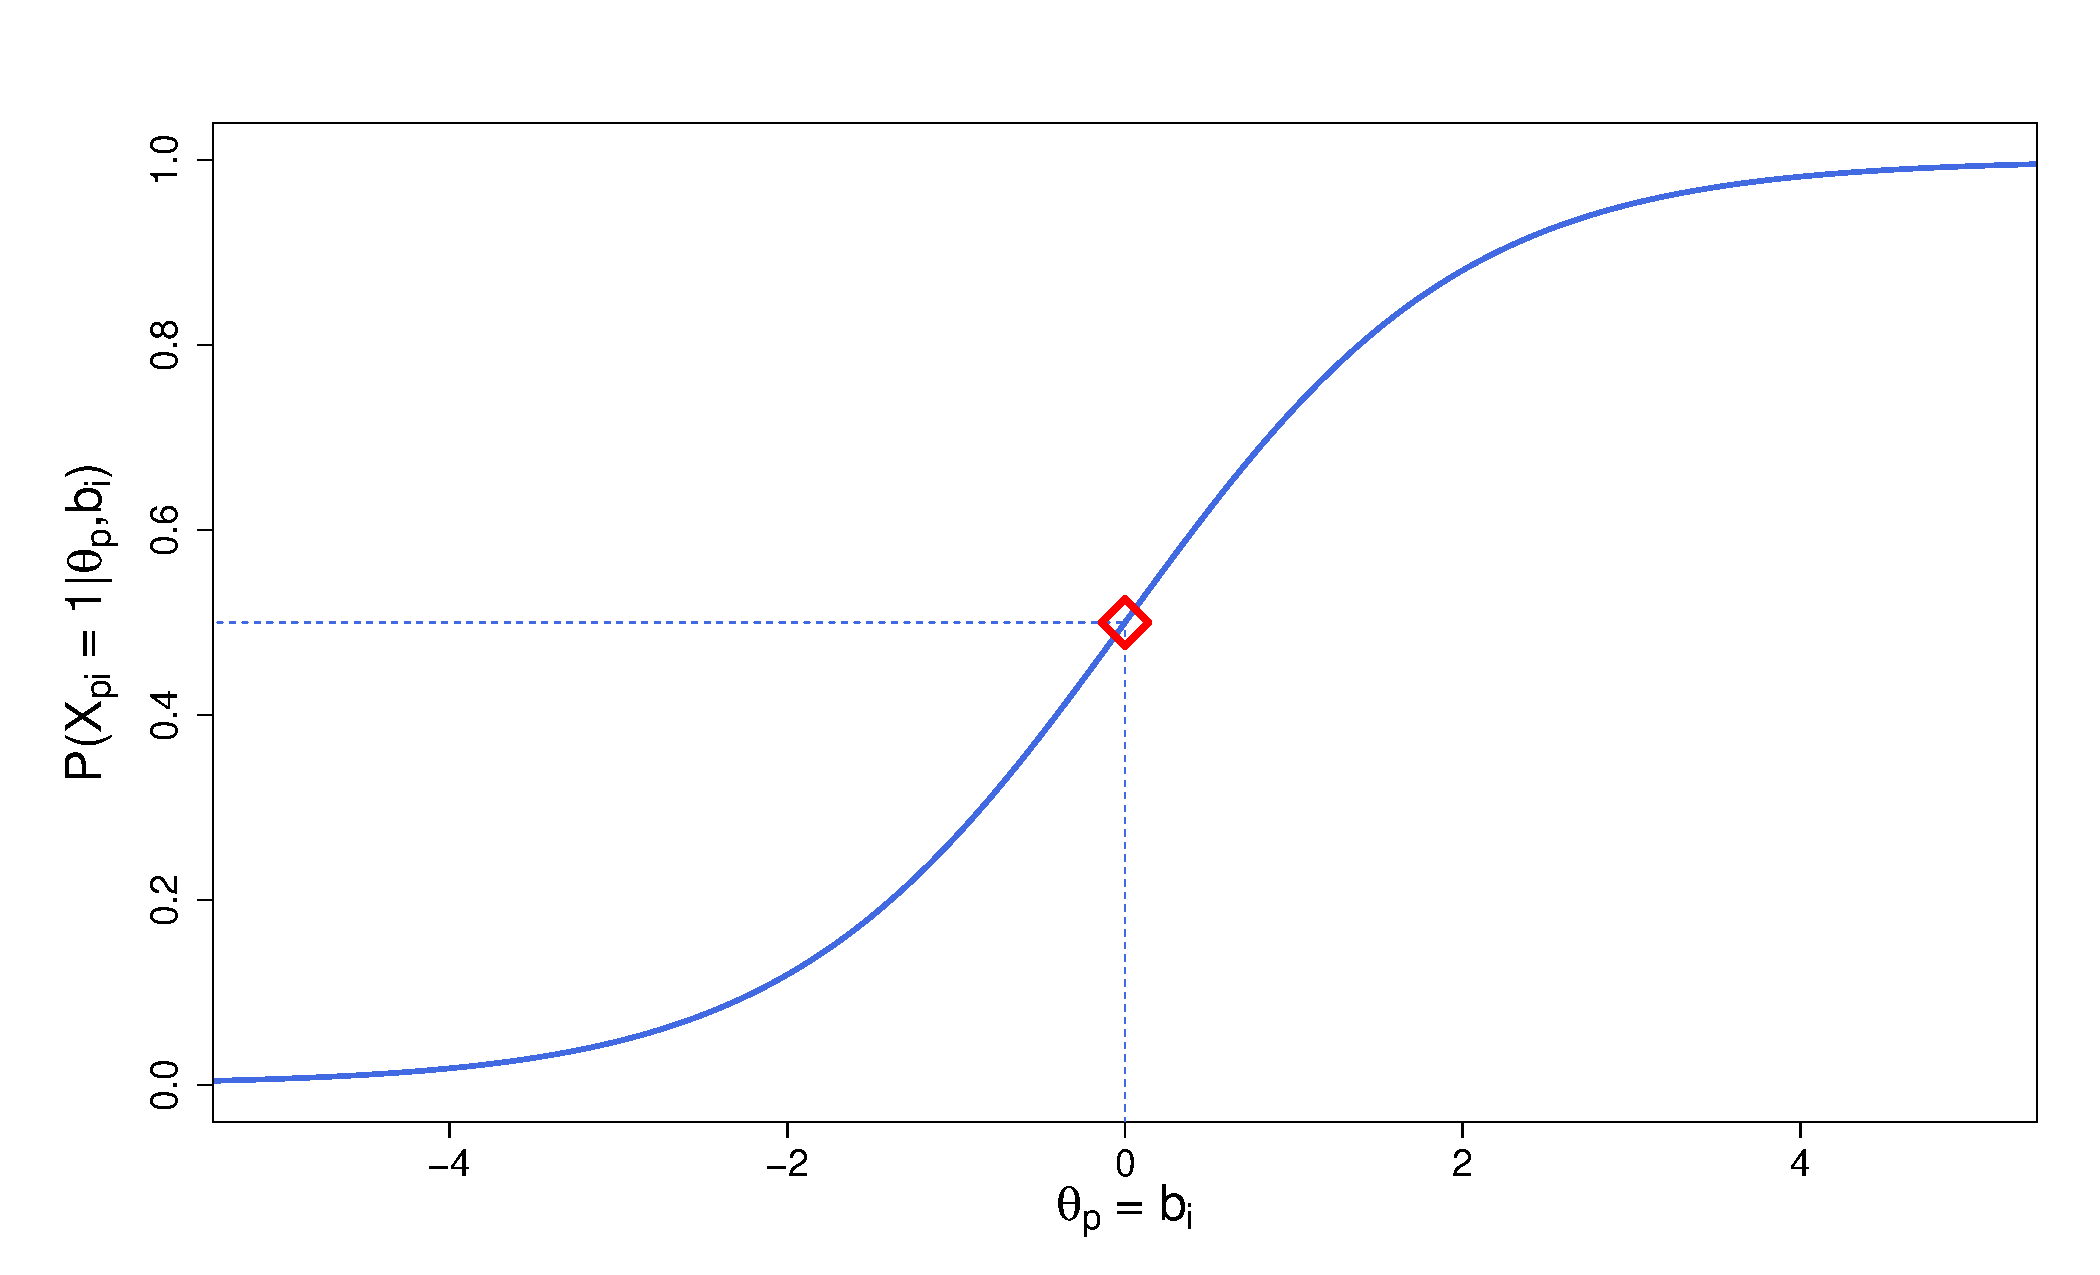
\includegraphics[width=.8\linewidth]{img/base.pdf}
		
		\centering
		\onslide<3>
		\centering
		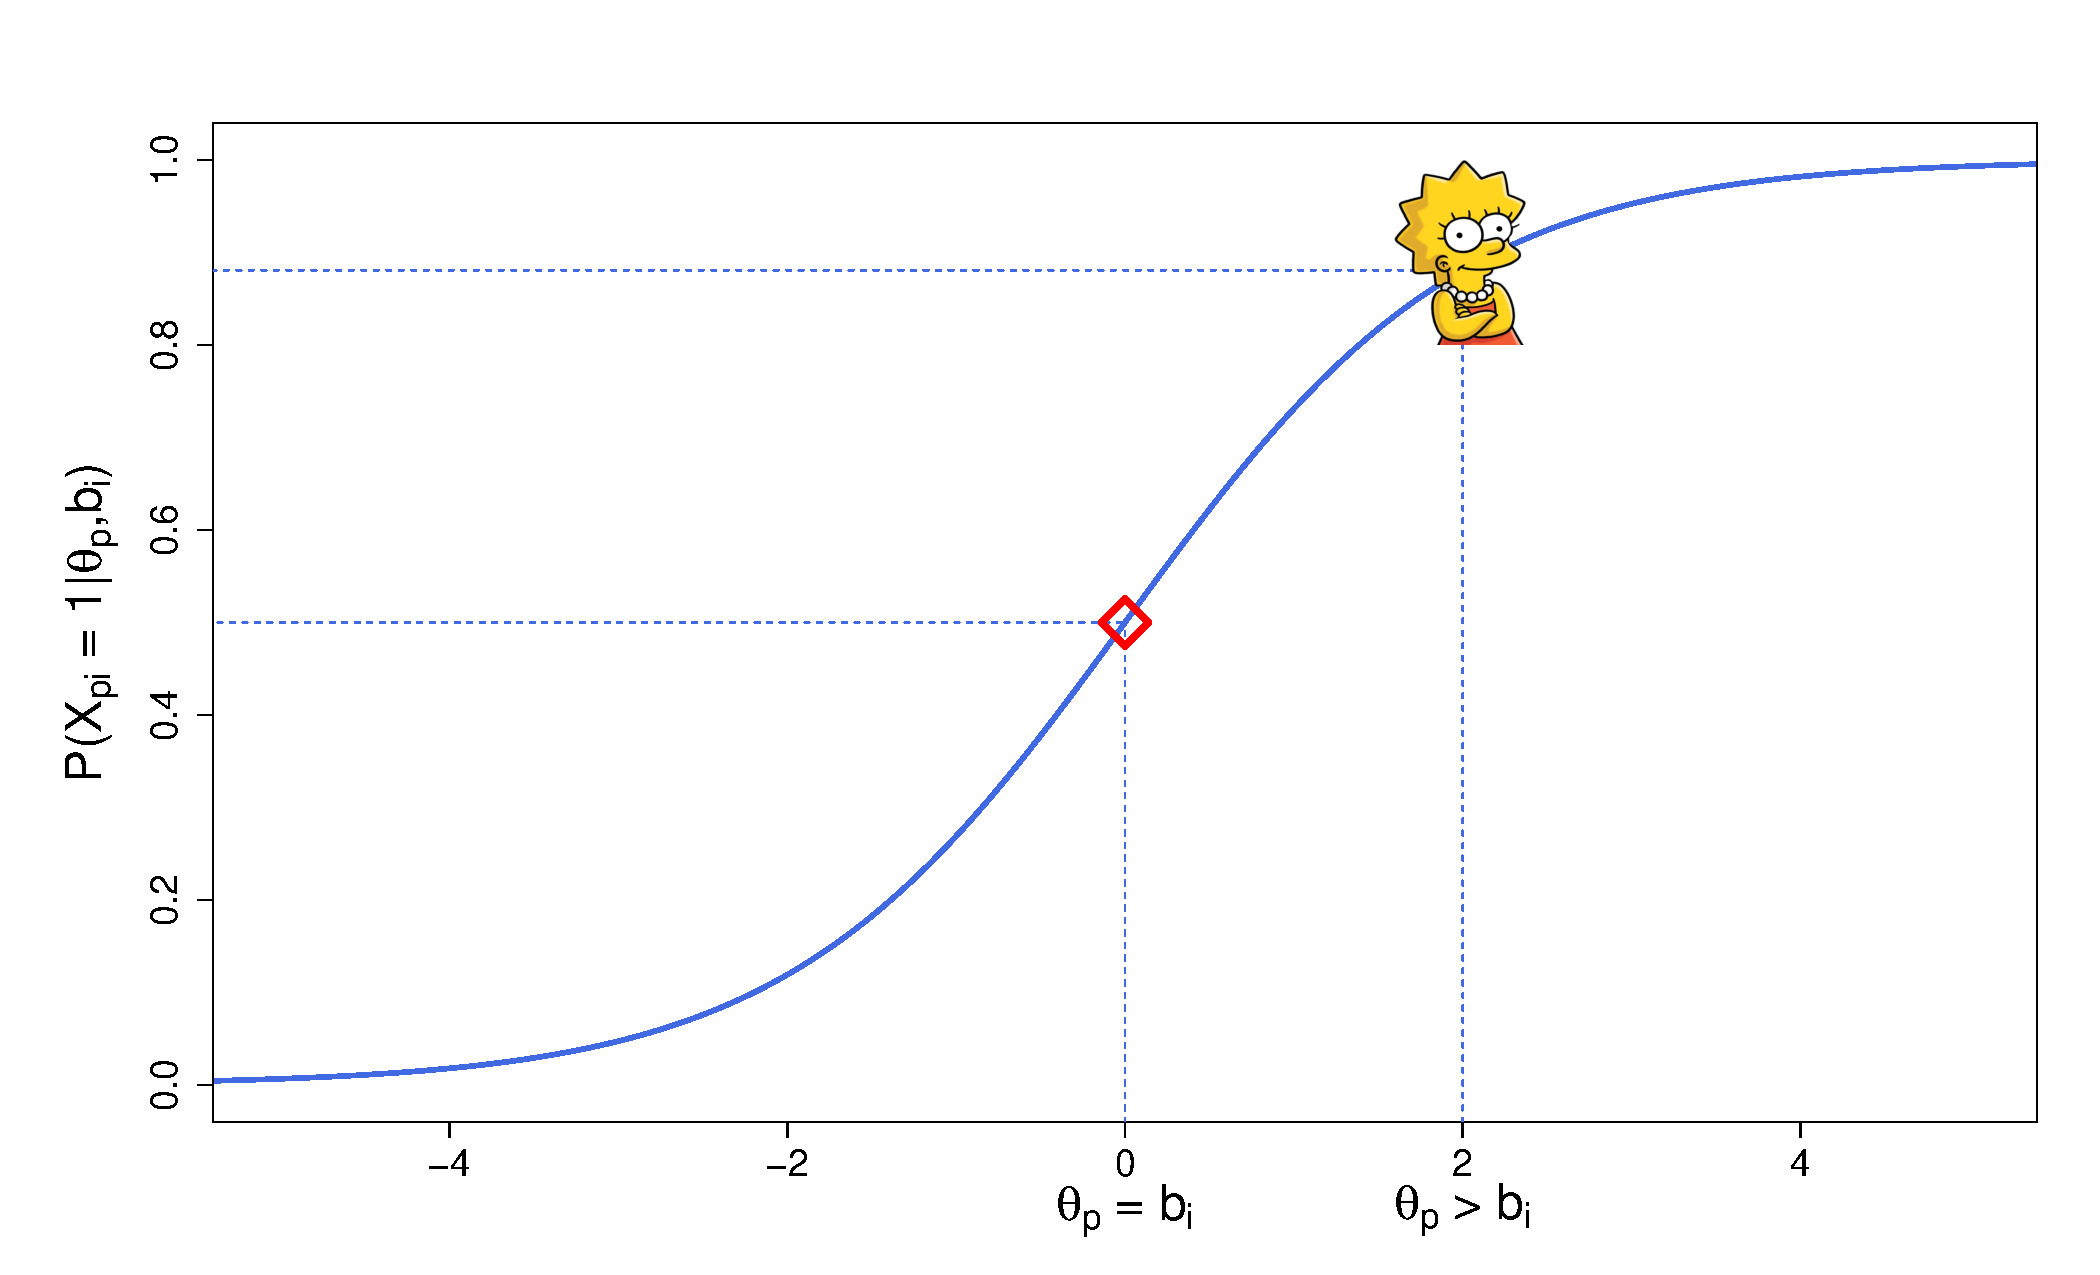
\includegraphics[width=.8\linewidth]{img/lisa.pdf}
		
		\centering
		\onslide<4>
		\centering
		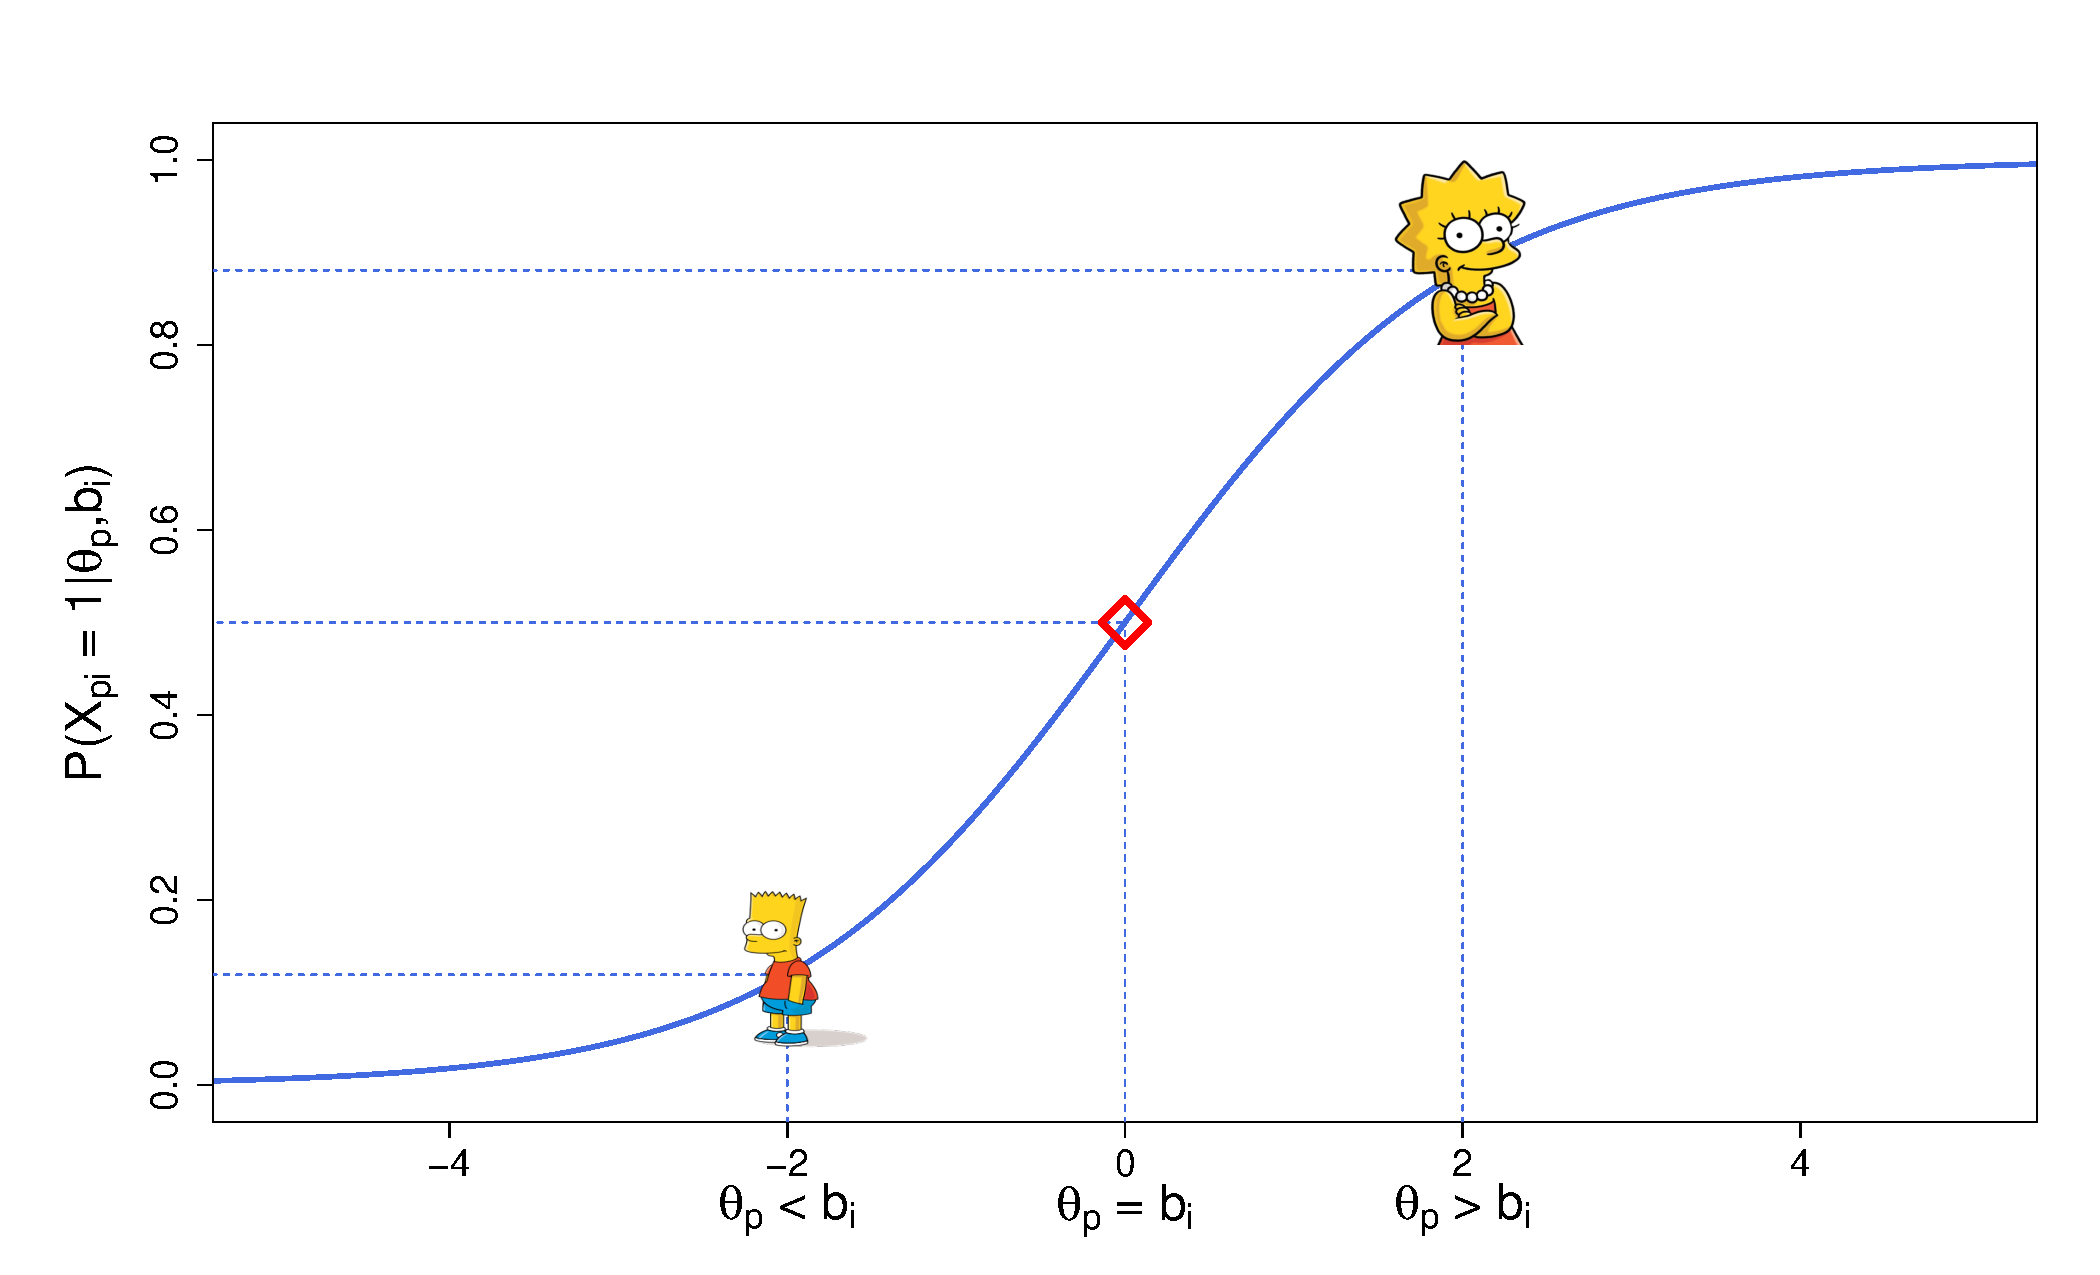
\includegraphics[width=.8\linewidth]{img/bart.pdf}
	\end{overprint}
	
\end{frame}


\begin{frame}{To each its own...IRT model}

Different IRT models according to:
	
\begin{itemize}
	\item Latent trait:
	\begin{itemize}
		\item \textcolor<2>{unipd}{Unidimensional model}
		\item  Multidimensional model	
	\end{itemize}
	
	\item Response categories: 
	
	\begin{itemize}
		\item  \textcolor<2>{unipd}{Dichotomous items} (Two response categories, e.g., true/falso, agree/disagree)
		\item Polytomous items (at least 3 response categories, e.g., Likert-type scale)
	\end{itemize}
\end{itemize} 

\end{frame}

\begin{frame}{Models for dichotomous responses}

IRT models can be distinguished according to the number of parameters describing the characteristics of the items. 
	
	\begin{itemize}
	\item One-Parameter Logistic Model (1-PL)
		
	\item Two-Parameter Logistic Model (2-PL; Birnbaum, 1968)
		
     \item Three-Parameter Logistic Model (3-PL; Lord, 1980)
		
	\item Four-Parameter Logistic Model (4-PL; Barton \& Lord, 1981)
	\end{itemize}
	

	
\end{frame}

\subsection*{1PL}

\begin{frame}
$$P(x_{pi} = 1| \theta_p, b_i) = \dfrac{\exp(\theta_p - b_i)}{1 + \exp(\theta_p - b_i)}$$

\begin{figure}
	\centering
	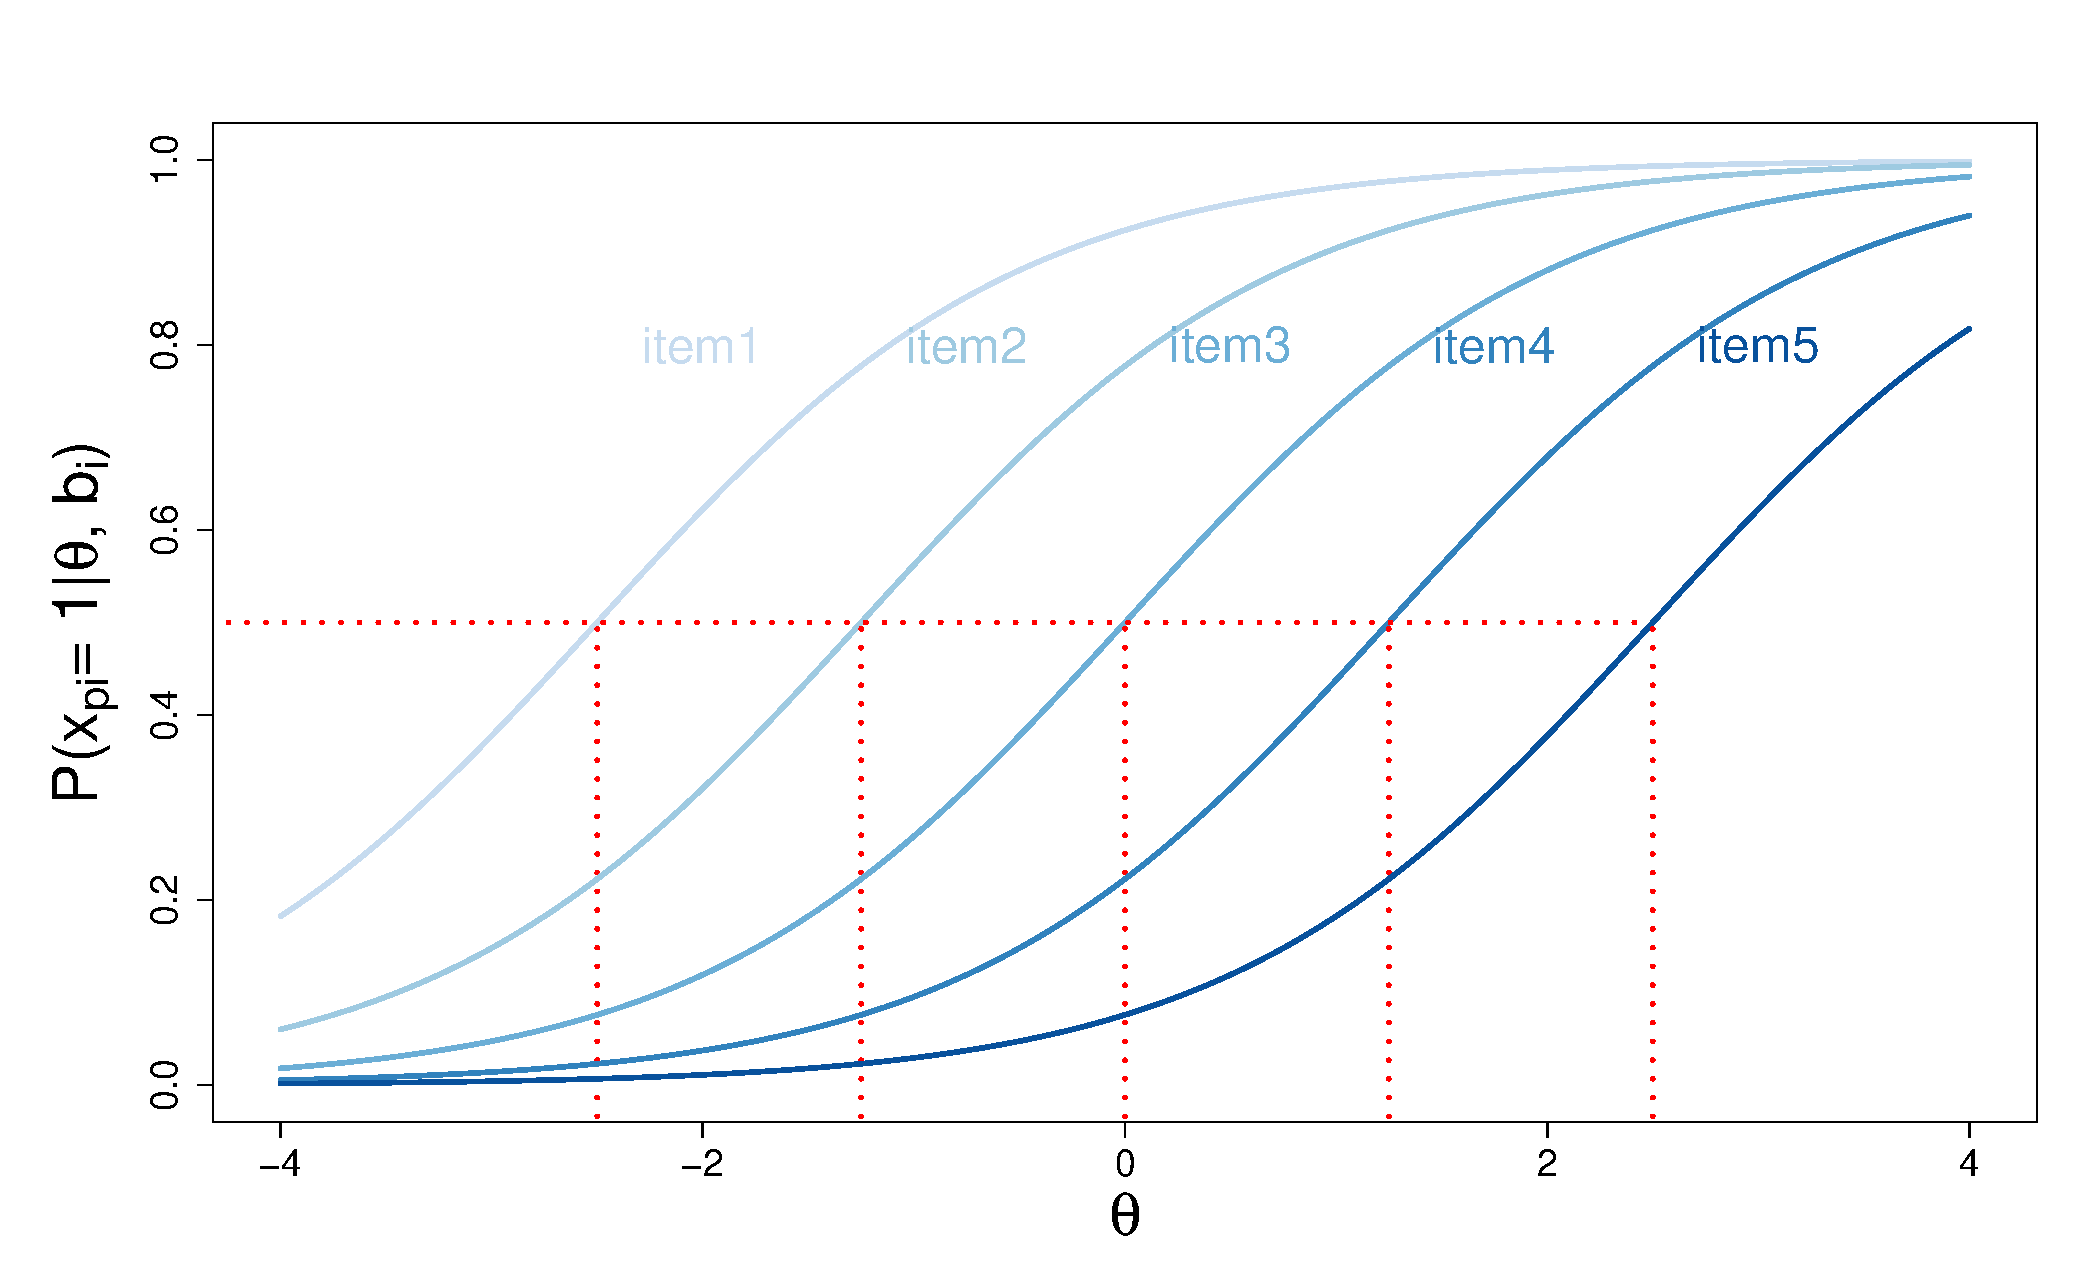
\includegraphics[width=.8\linewidth]{img/icc-1pl}
\end{figure}
\end{frame}



\subsection*{2PL}

\begin{frame}
$$P(x_{pi} = 1|\theta_p, b_i, a_i) = \frac{\exp[a_i(\theta_p - b_i)]}{1 + \exp[a_i(\theta_p - b_i)]}$$


\pause

\begin{overprint}
	
	\onslide<1>
	\centering
	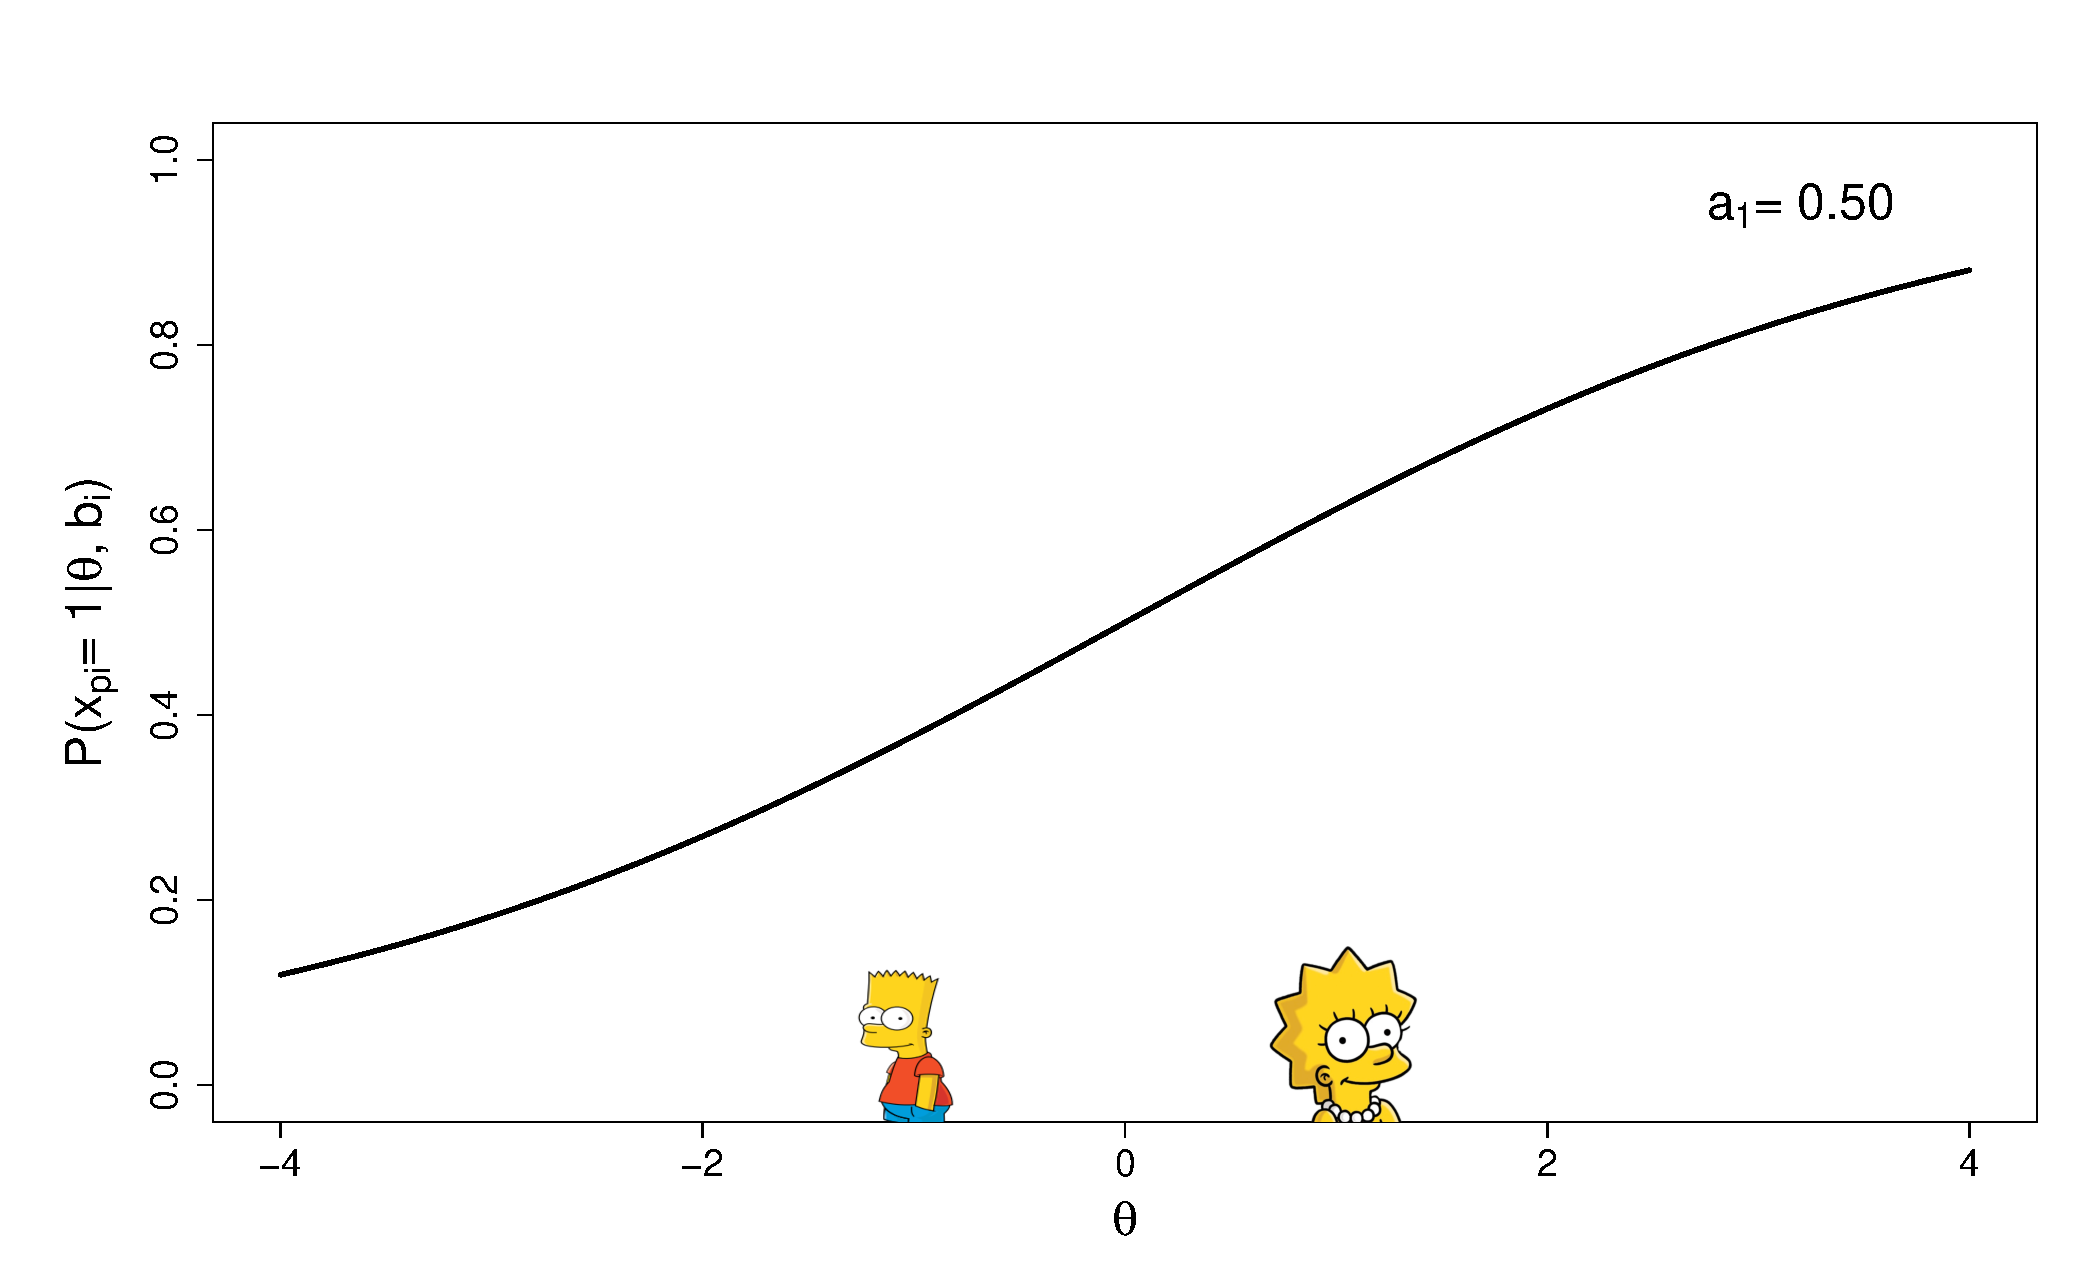
\includegraphics[width=.75\linewidth]{img/lisa-bart-base}
	\onslide<2>
	\centering
	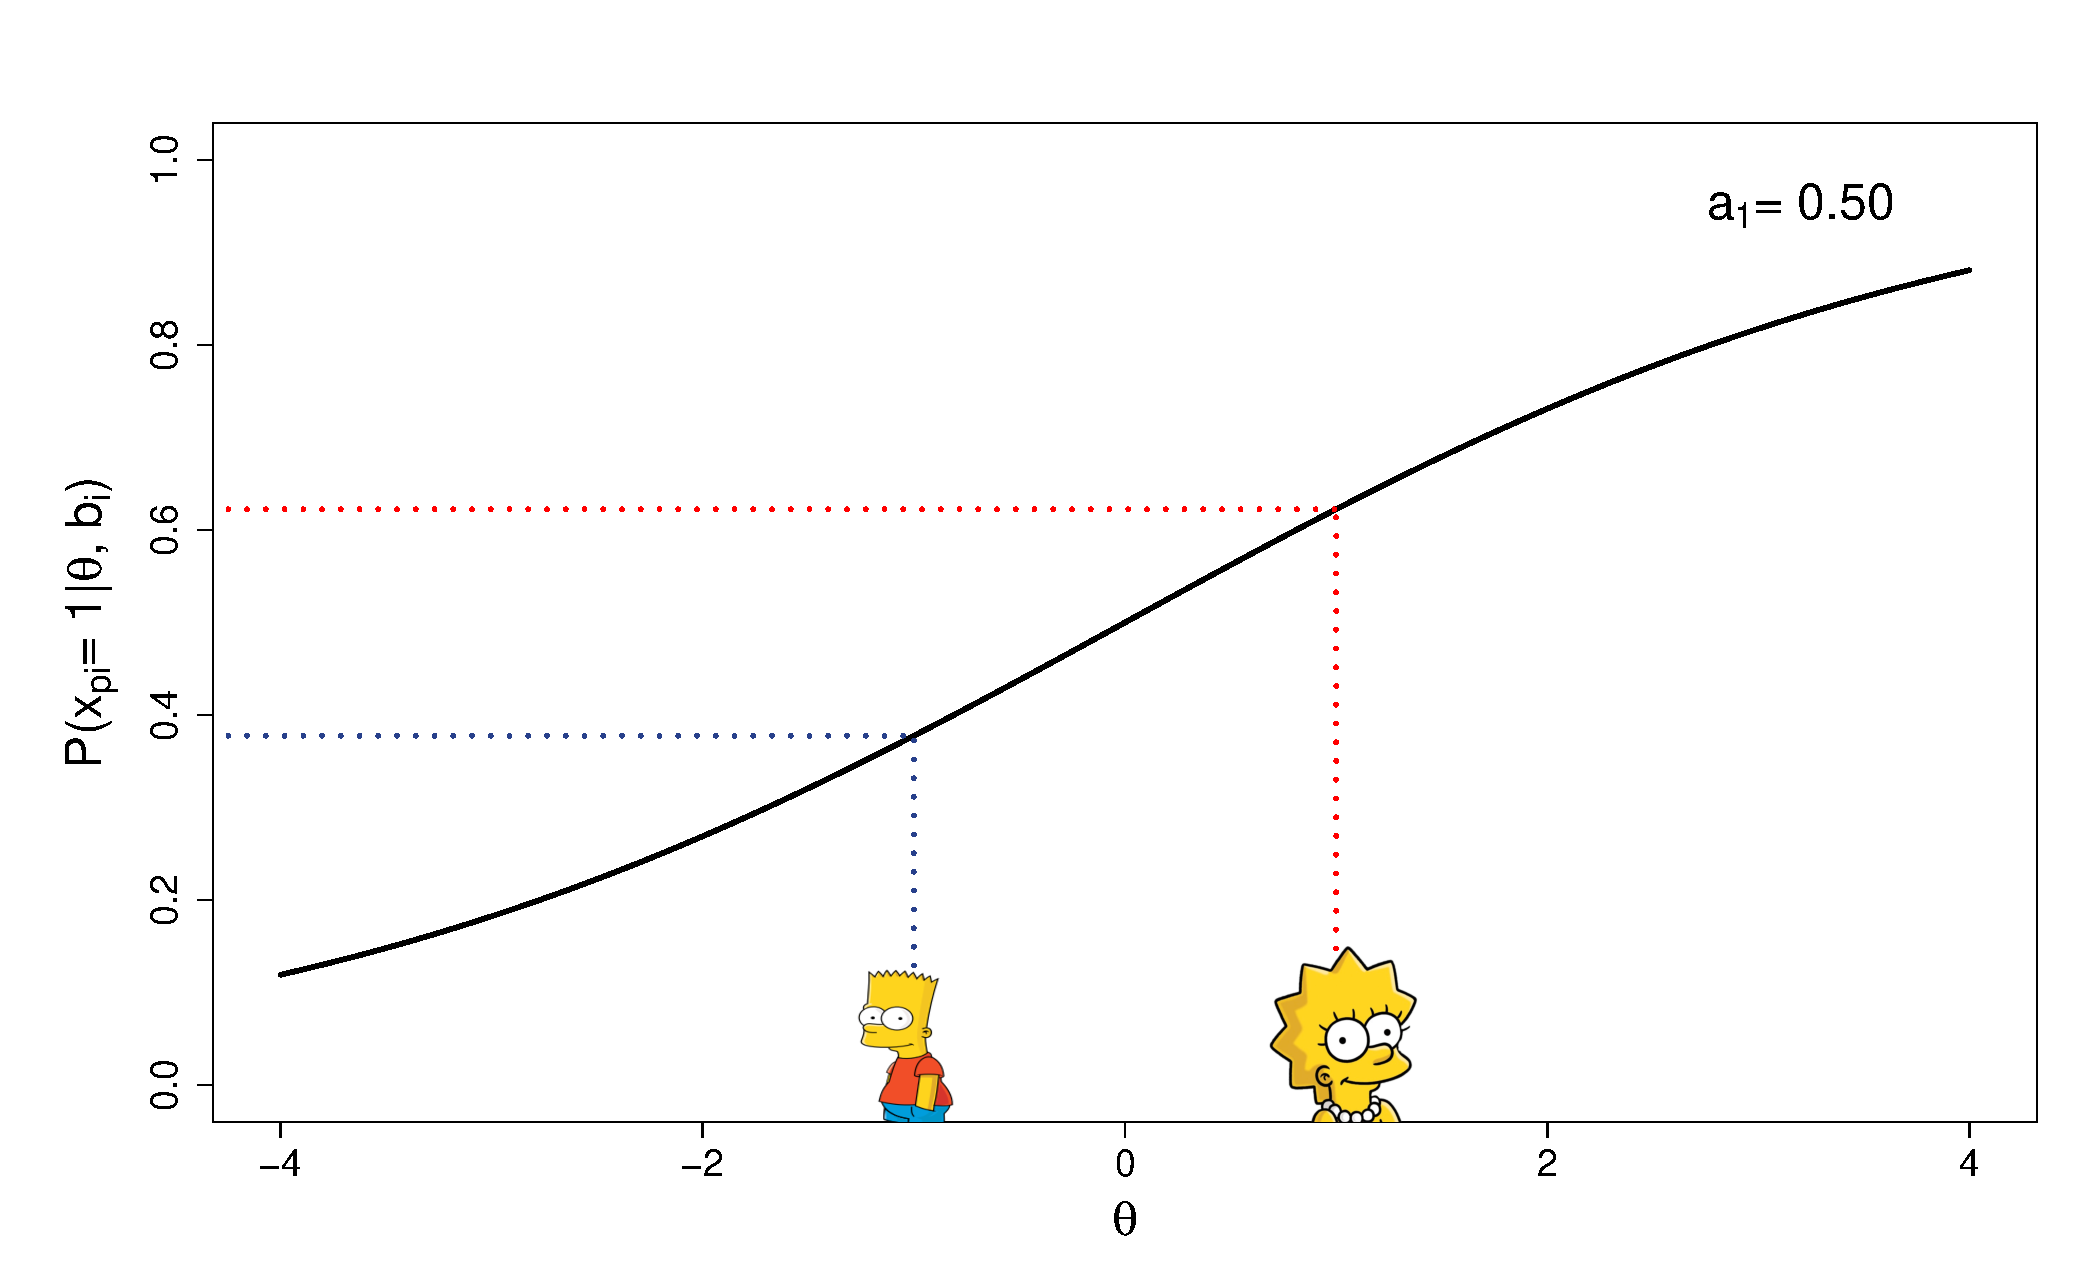
\includegraphics[width=.75\linewidth]{img/lisa-bart-icc}
	\onslide<3>
	\centering
	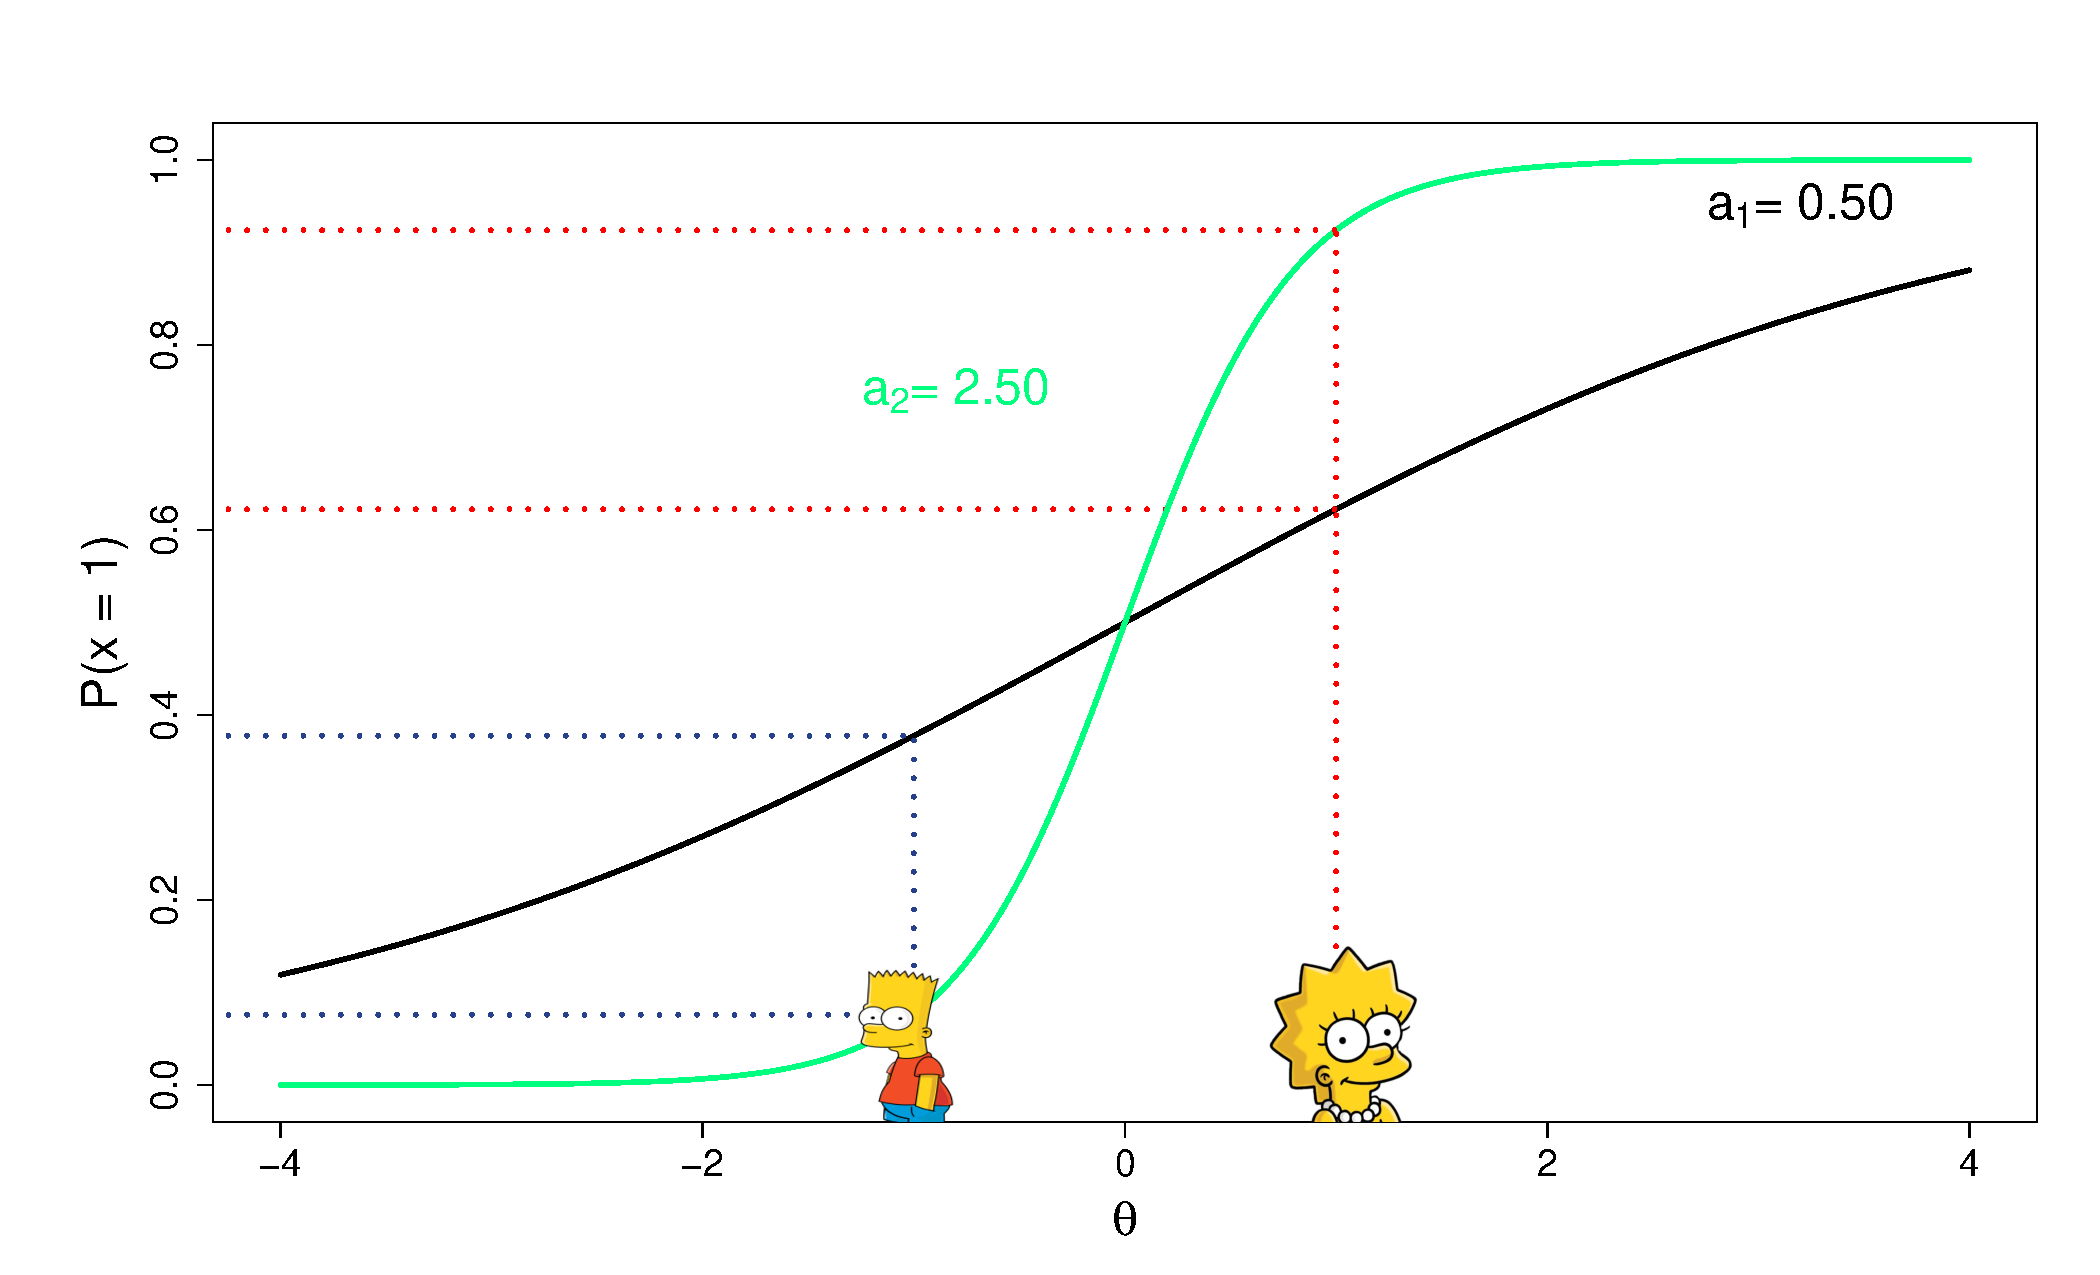
\includegraphics[width=.75\linewidth]{img/lisa-bart-icc-1}
\end{overprint}
\end{frame}


\begin{frame}
	\centering
	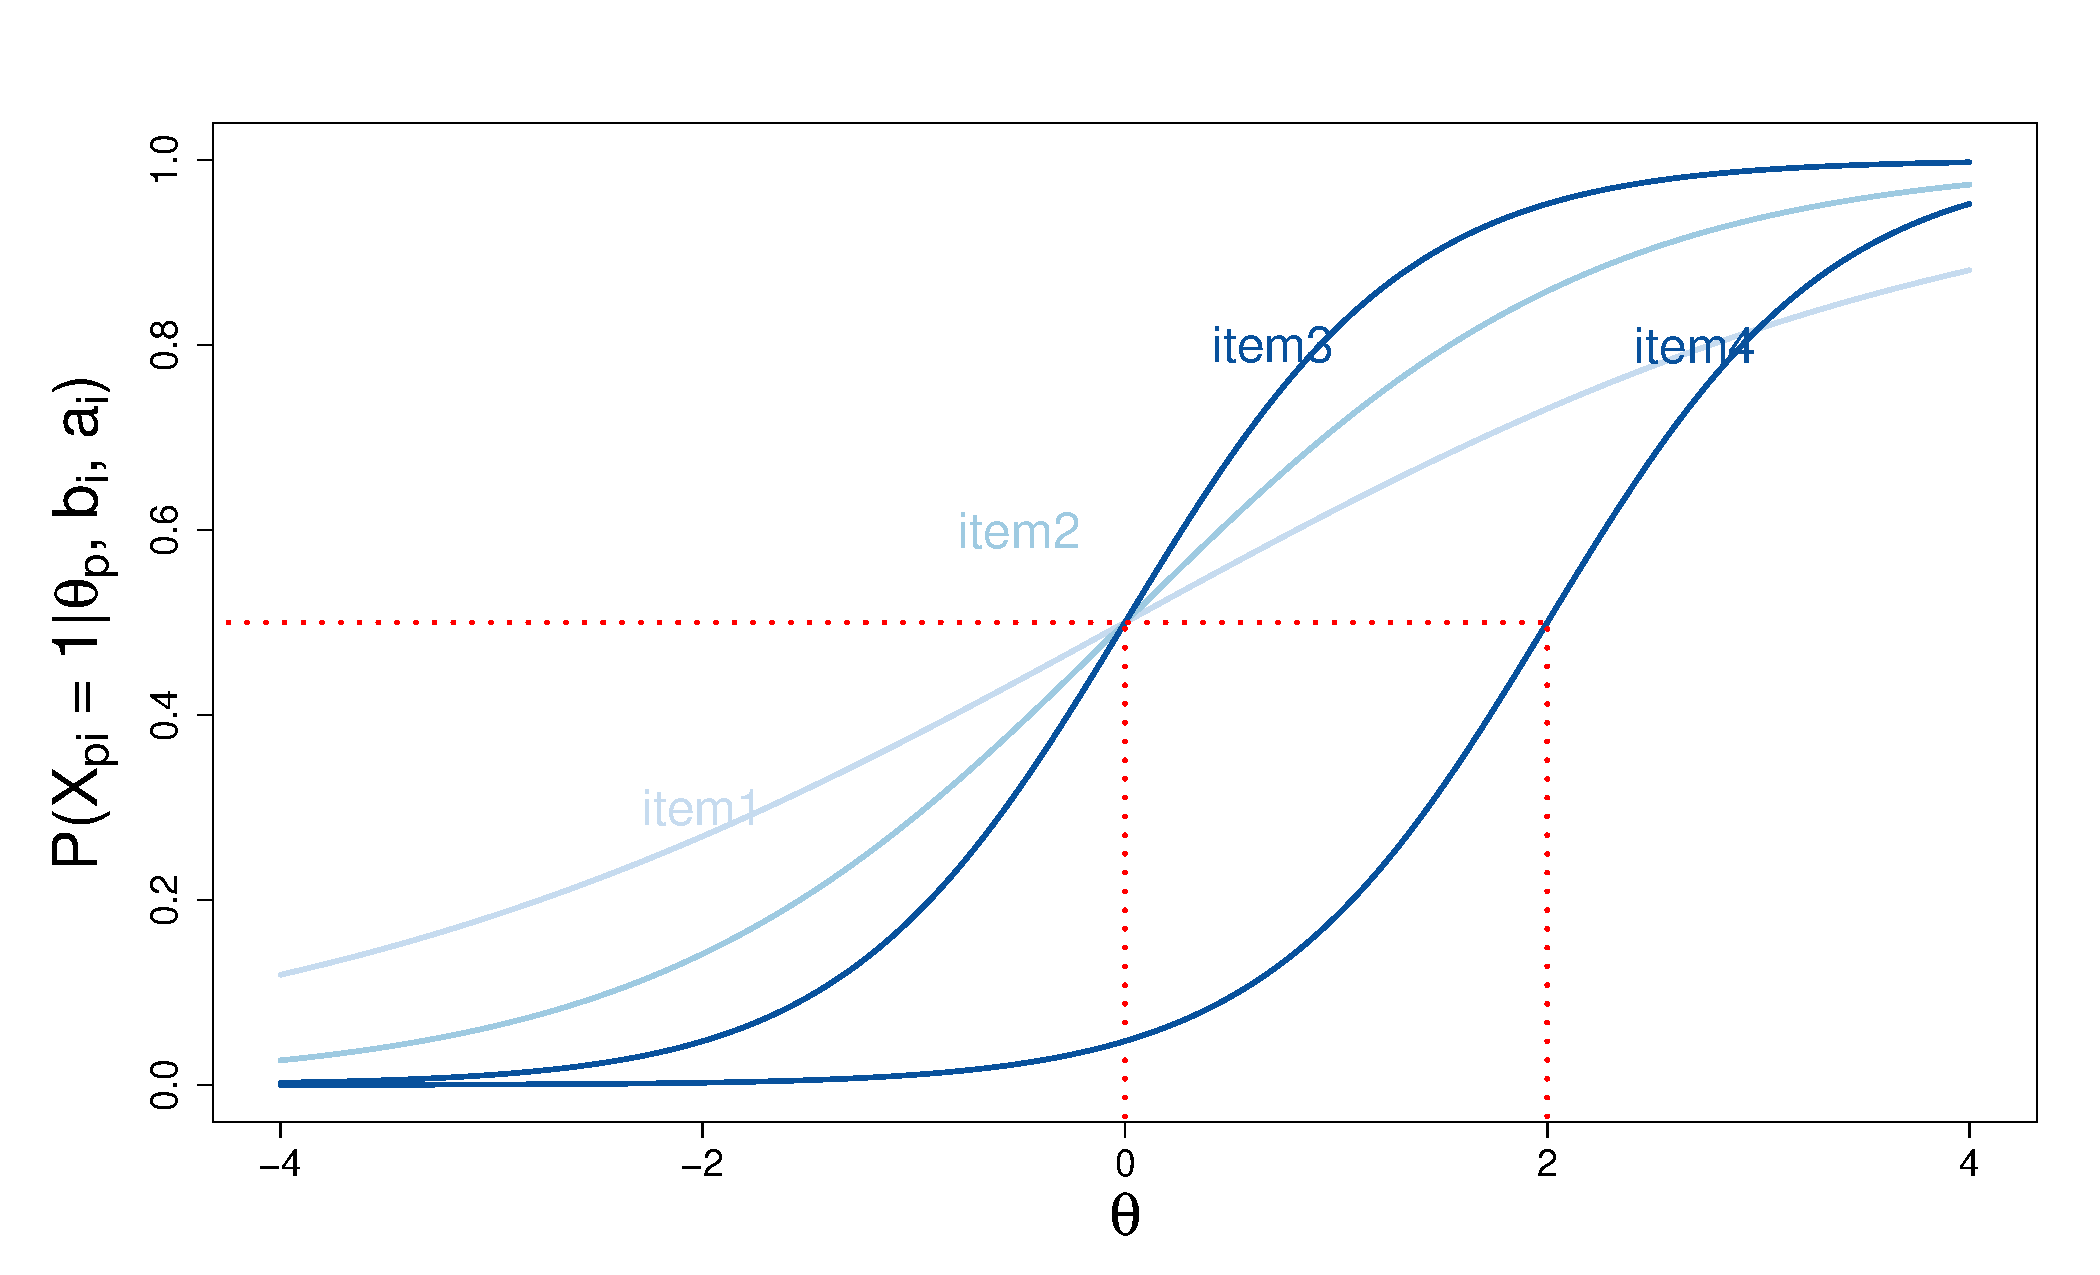
\includegraphics[width=.8\linewidth]{img/ICC-2pl.pdf}
	
\end{frame}

\subsection*{Moving the asymptotes}

\begin{frame}


\begin{overprint}
	\onslide<1>
	
	\begin{center}
		\textbf{3-PL}
	\end{center}
	\small
	$$P(x_{pi} = 1| \theta_p, b_i, a_i) = c_i + (1 - c_i) \dfrac{\exp[a_i(\theta_p - b_i)]}{1+\exp[a_i(\theta_p - b_i)]}$$
	
	\centering
	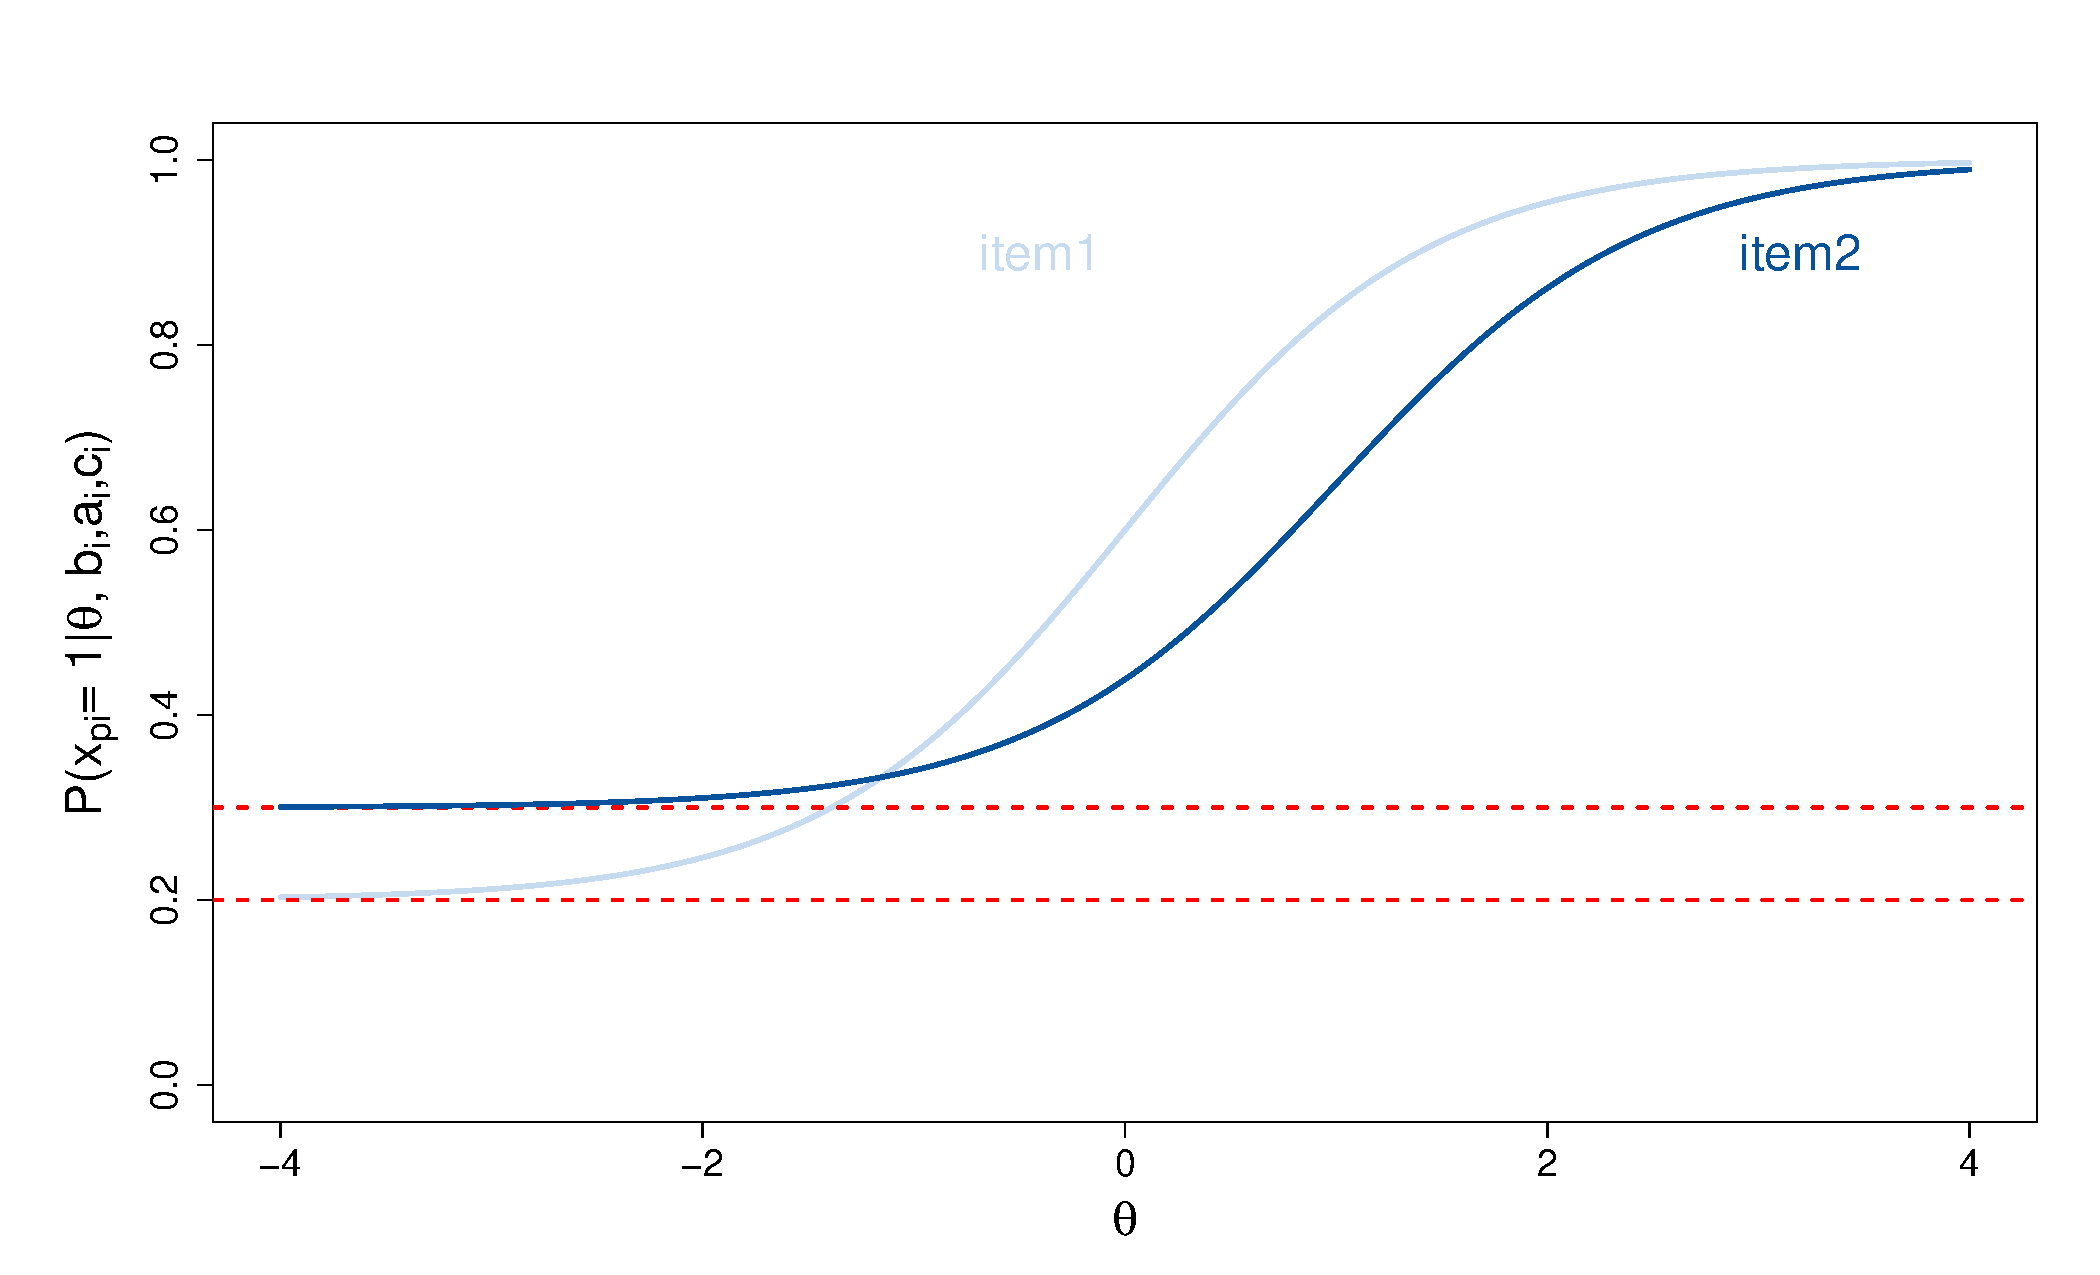
\includegraphics[width=.75\linewidth]{img/icc-3pl}
	
	\onslide<2>
		\begin{center}
		\textbf{4-PL}
	\end{center}
	\small
	$$P(x_{pi} = 1| \theta_p, b_i, a_i) = c_i + (d_i - c_i) \dfrac{\exp[a_i(\theta_p - b_i)]}{1+\exp[a_i(\theta_p - b_i)]}$$
	
		\centering
	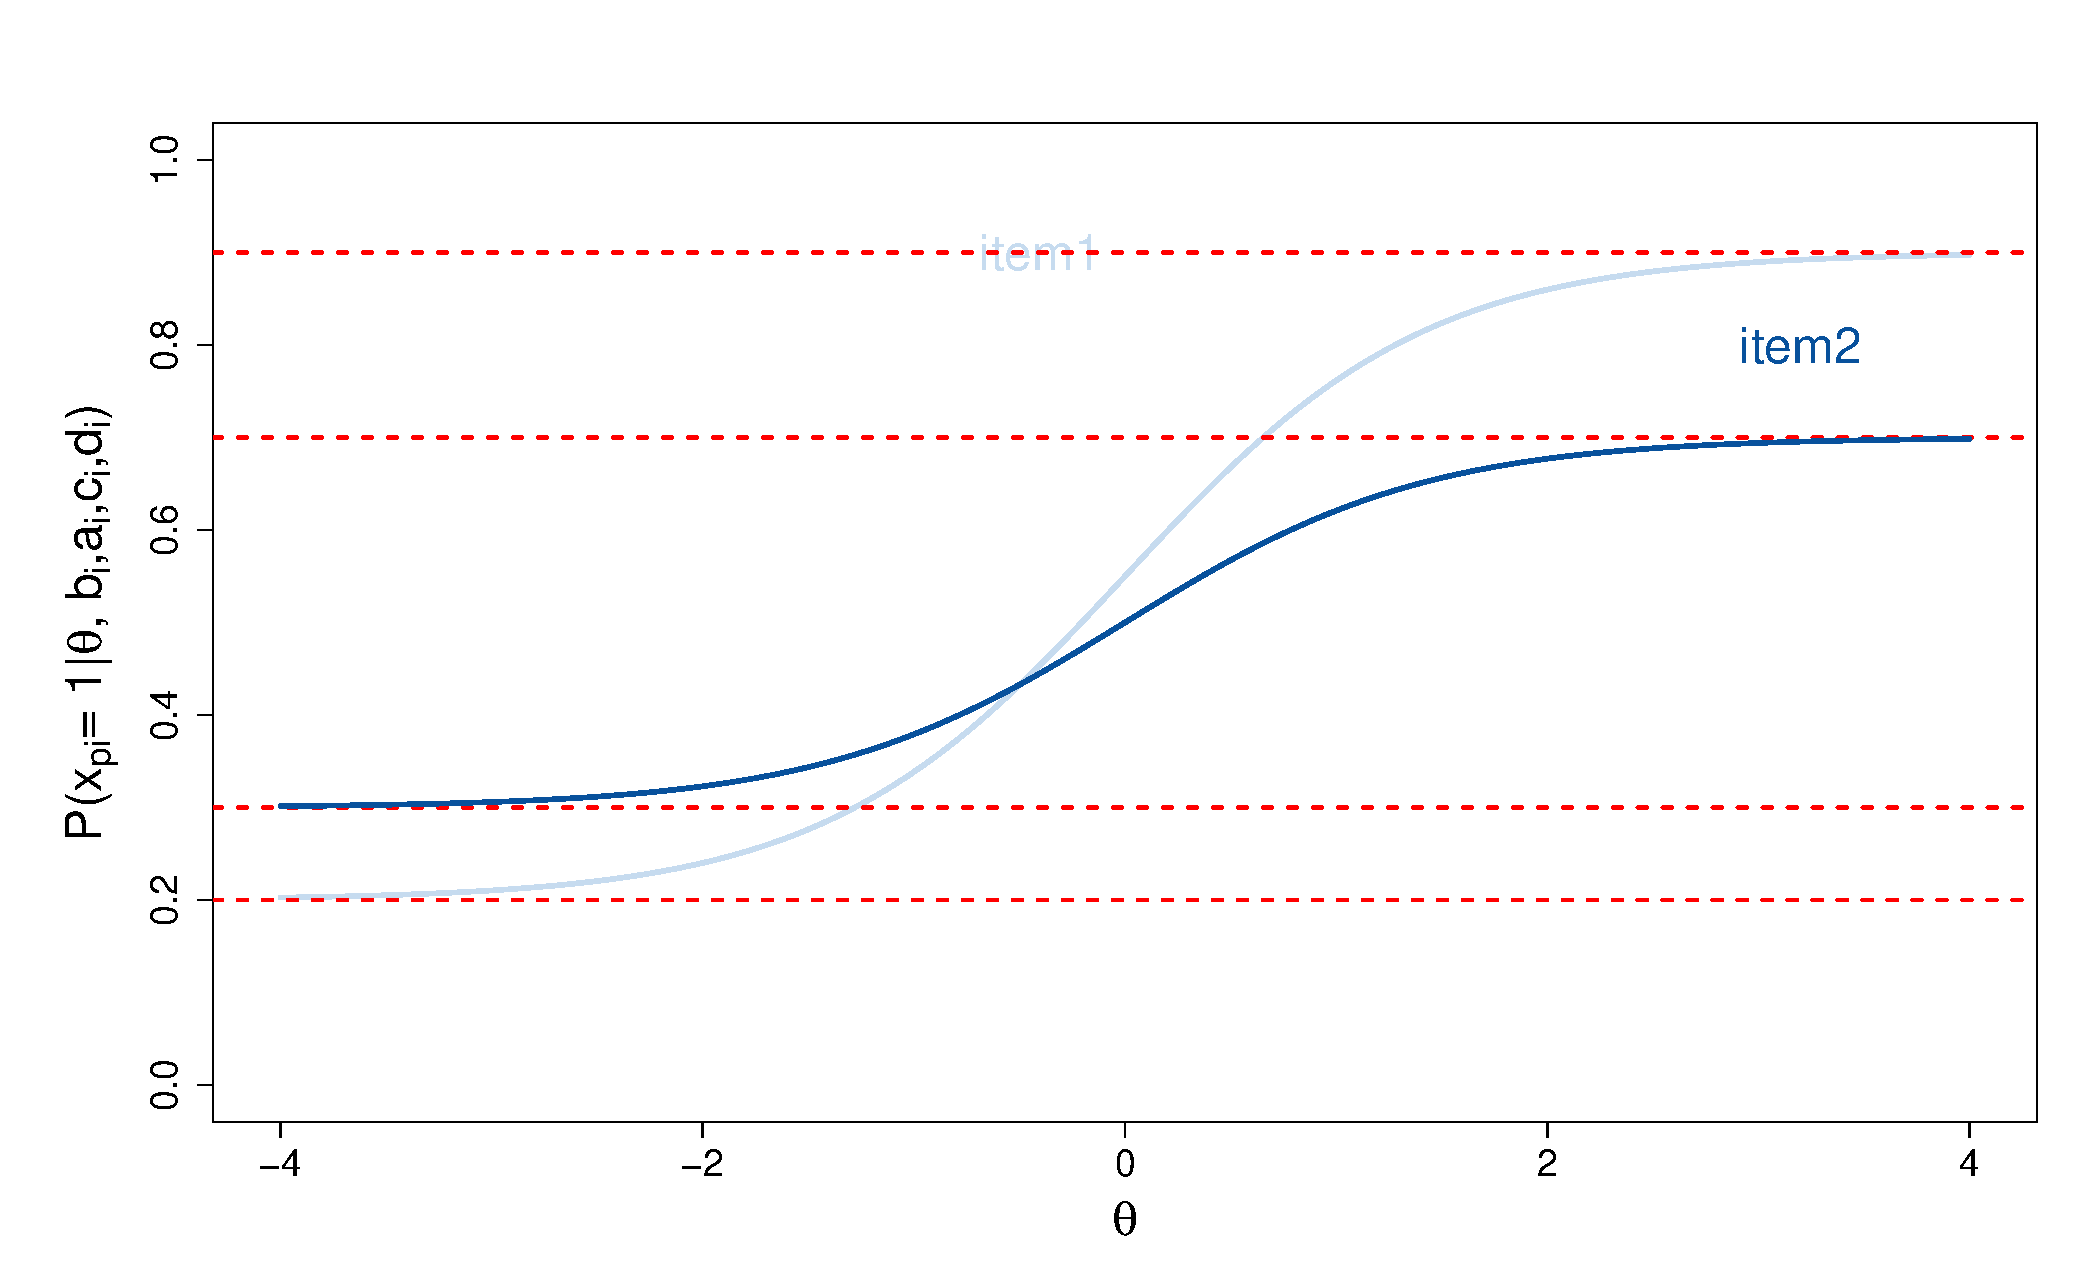
\includegraphics[width=.75\linewidth]{img/icc-4pl}
\end{overprint}

		
		

\end{frame}


\section[IFs]{Item and Test Information Functions}

\subsection*{1PL}

\begin{frame}
	
	\centering
	\begin{overprint}
		
		\centering
		\onslide<1>
	
		\vspace*{3mm}
		
		Item Information Function:	\\
		$I_i(\theta) = P_i(\theta, b_i)[1-P_i(\theta, b_i)]$
		
		\centering
		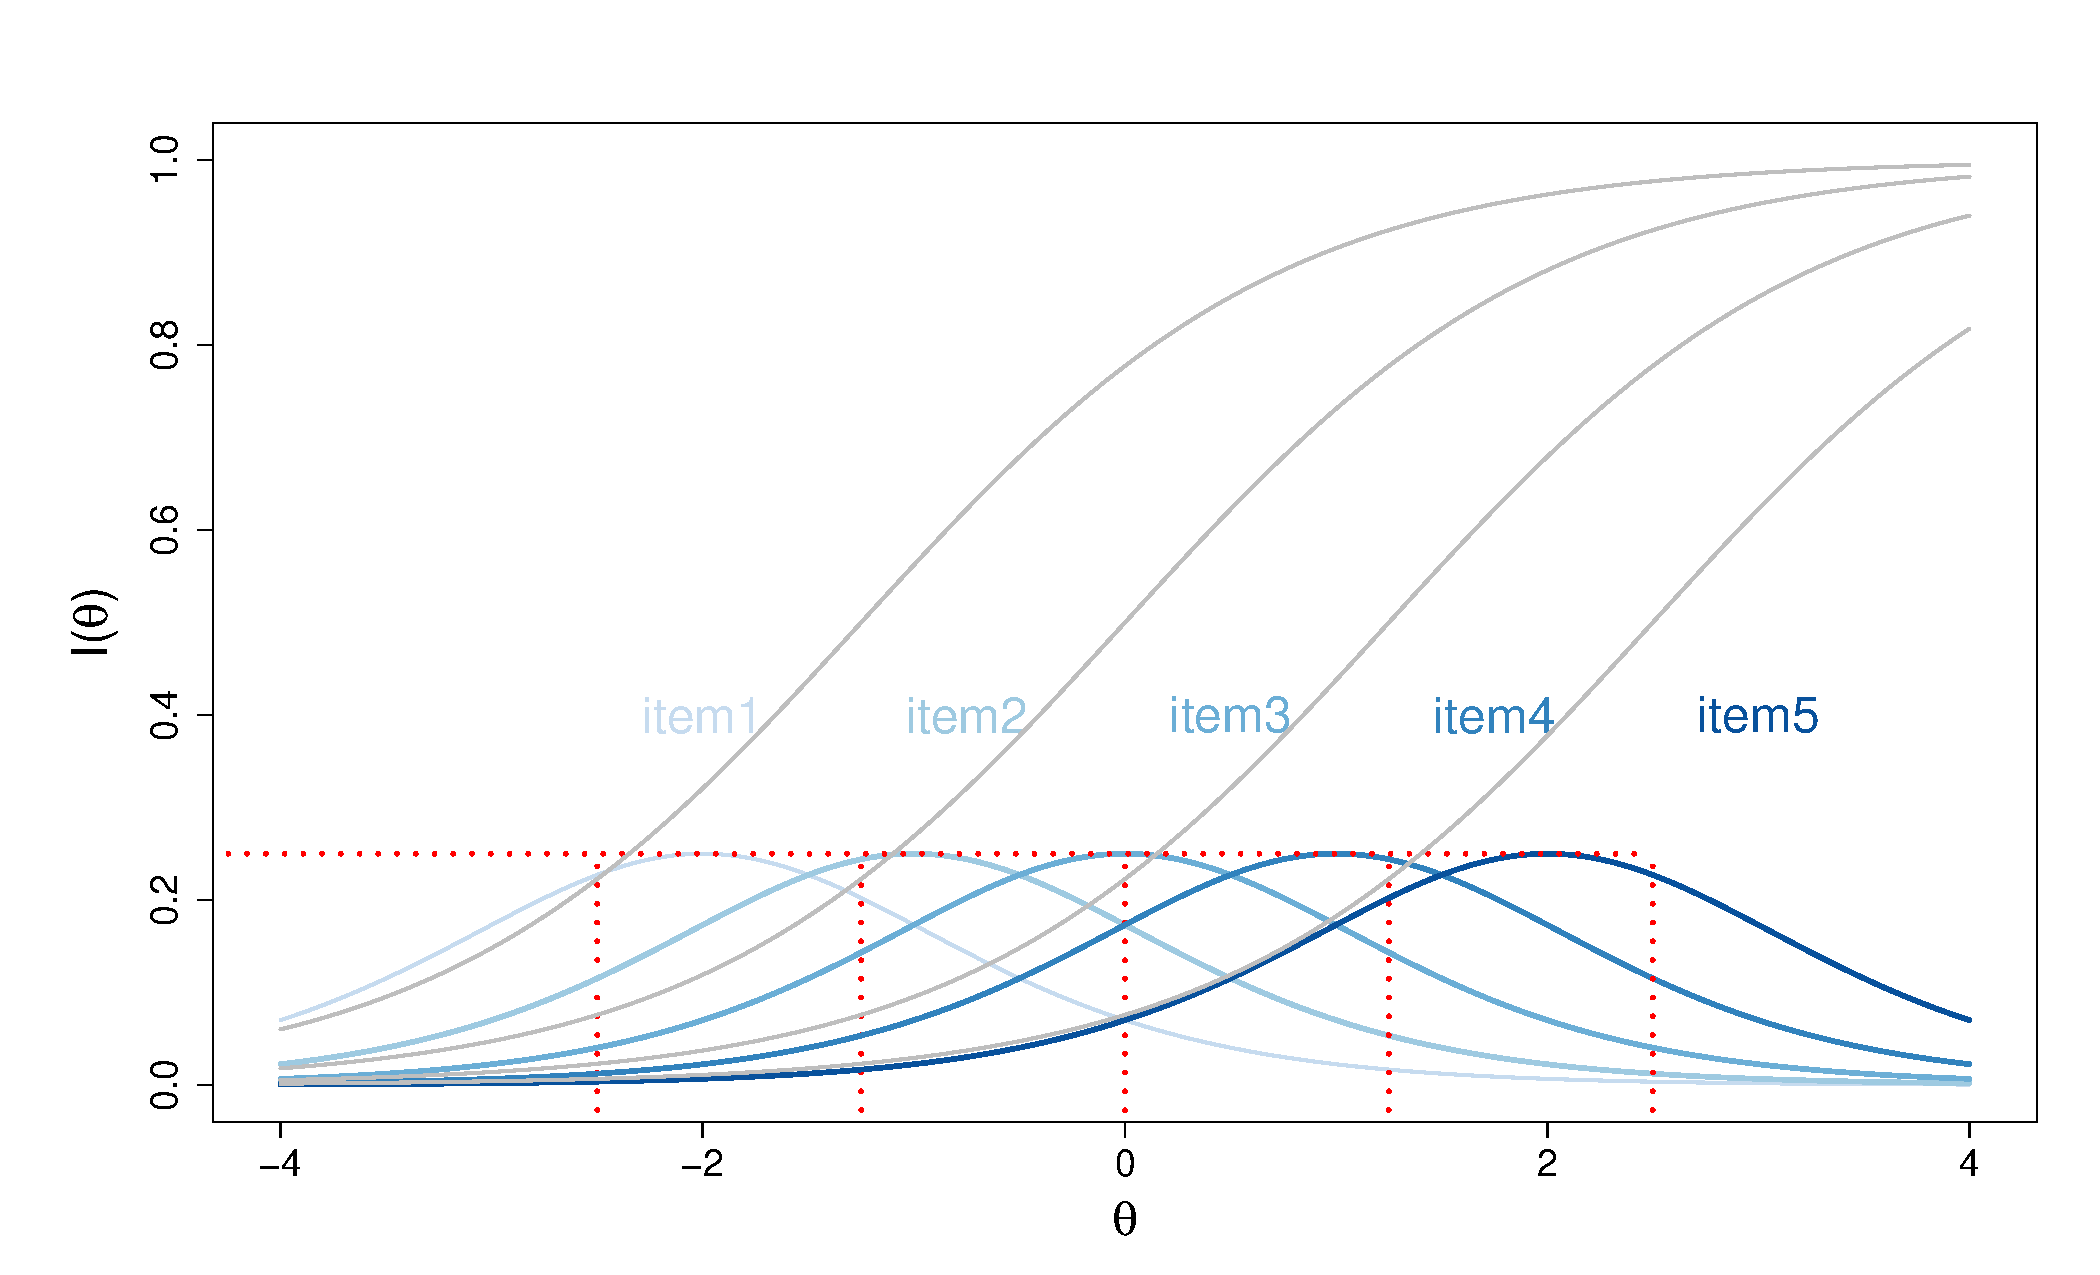
\includegraphics[width=.80\linewidth]{img/iif-1pl.pdf}
		
		\onslide<2>
		\vspace*{3mm}
		Test Information Function:	\\	$I(\theta) =  \sum_{i = 1}^{I} I_i(\theta)$
		
		\centering
		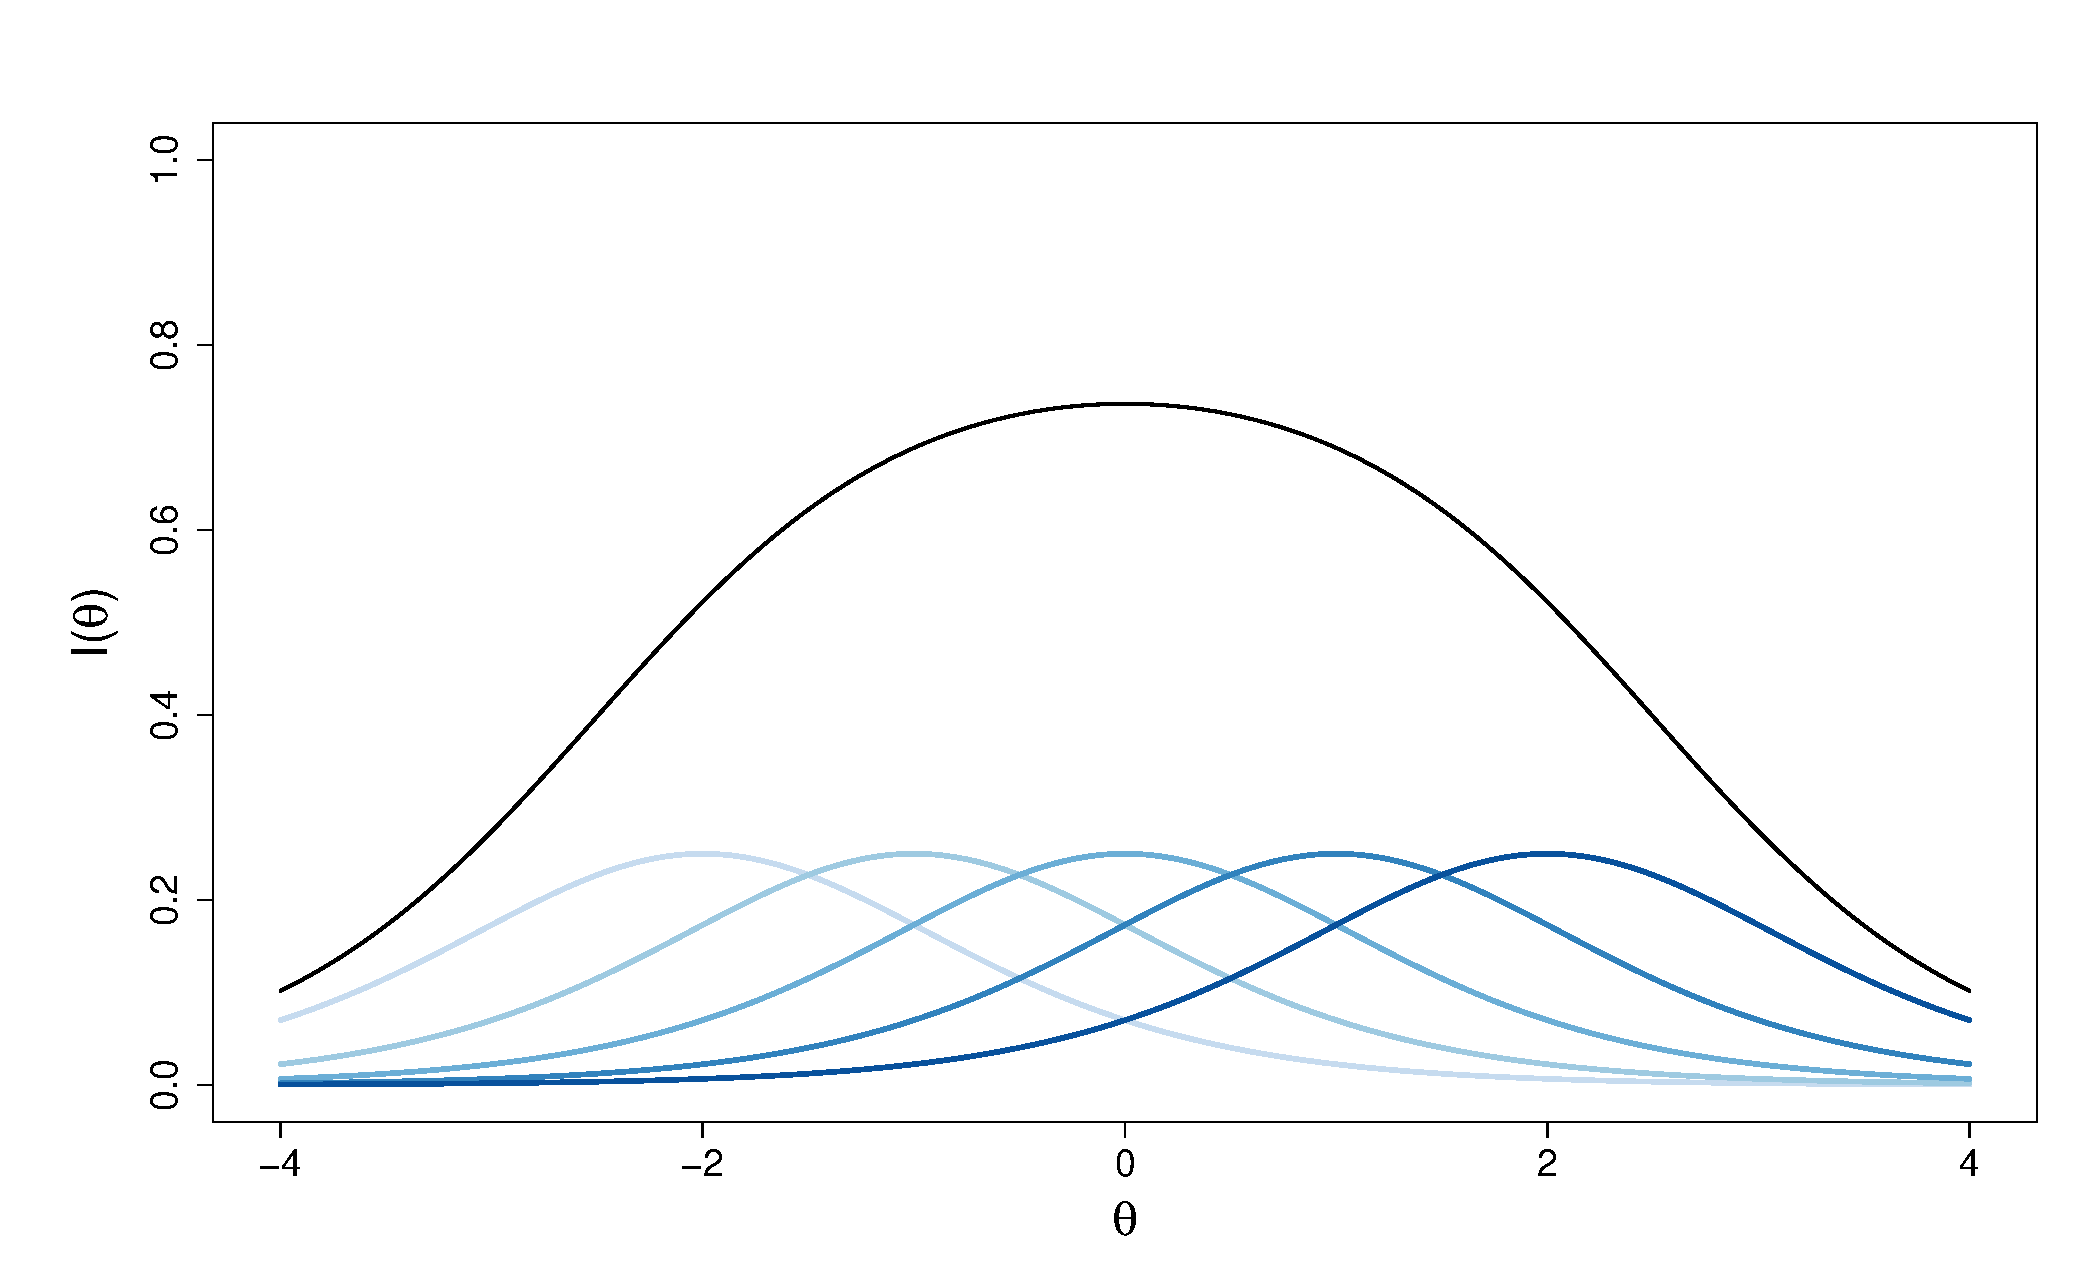
\includegraphics[width=.80\linewidth]{img/tif-1pl.pdf}
	\end{overprint}
\end{frame}

\subsection*{2PL}


\begin{frame}
	
	\centering
	\begin{overprint}
		
		\centering
		\onslide<1>
		
		\vspace*{3mm}
		
		Item Information Function:	\\
		$I_i(\theta) = a_i^2P_i(\theta, b_i, a_i)[1-P_i(\theta, b_i, a_i)]$
		
		\centering
		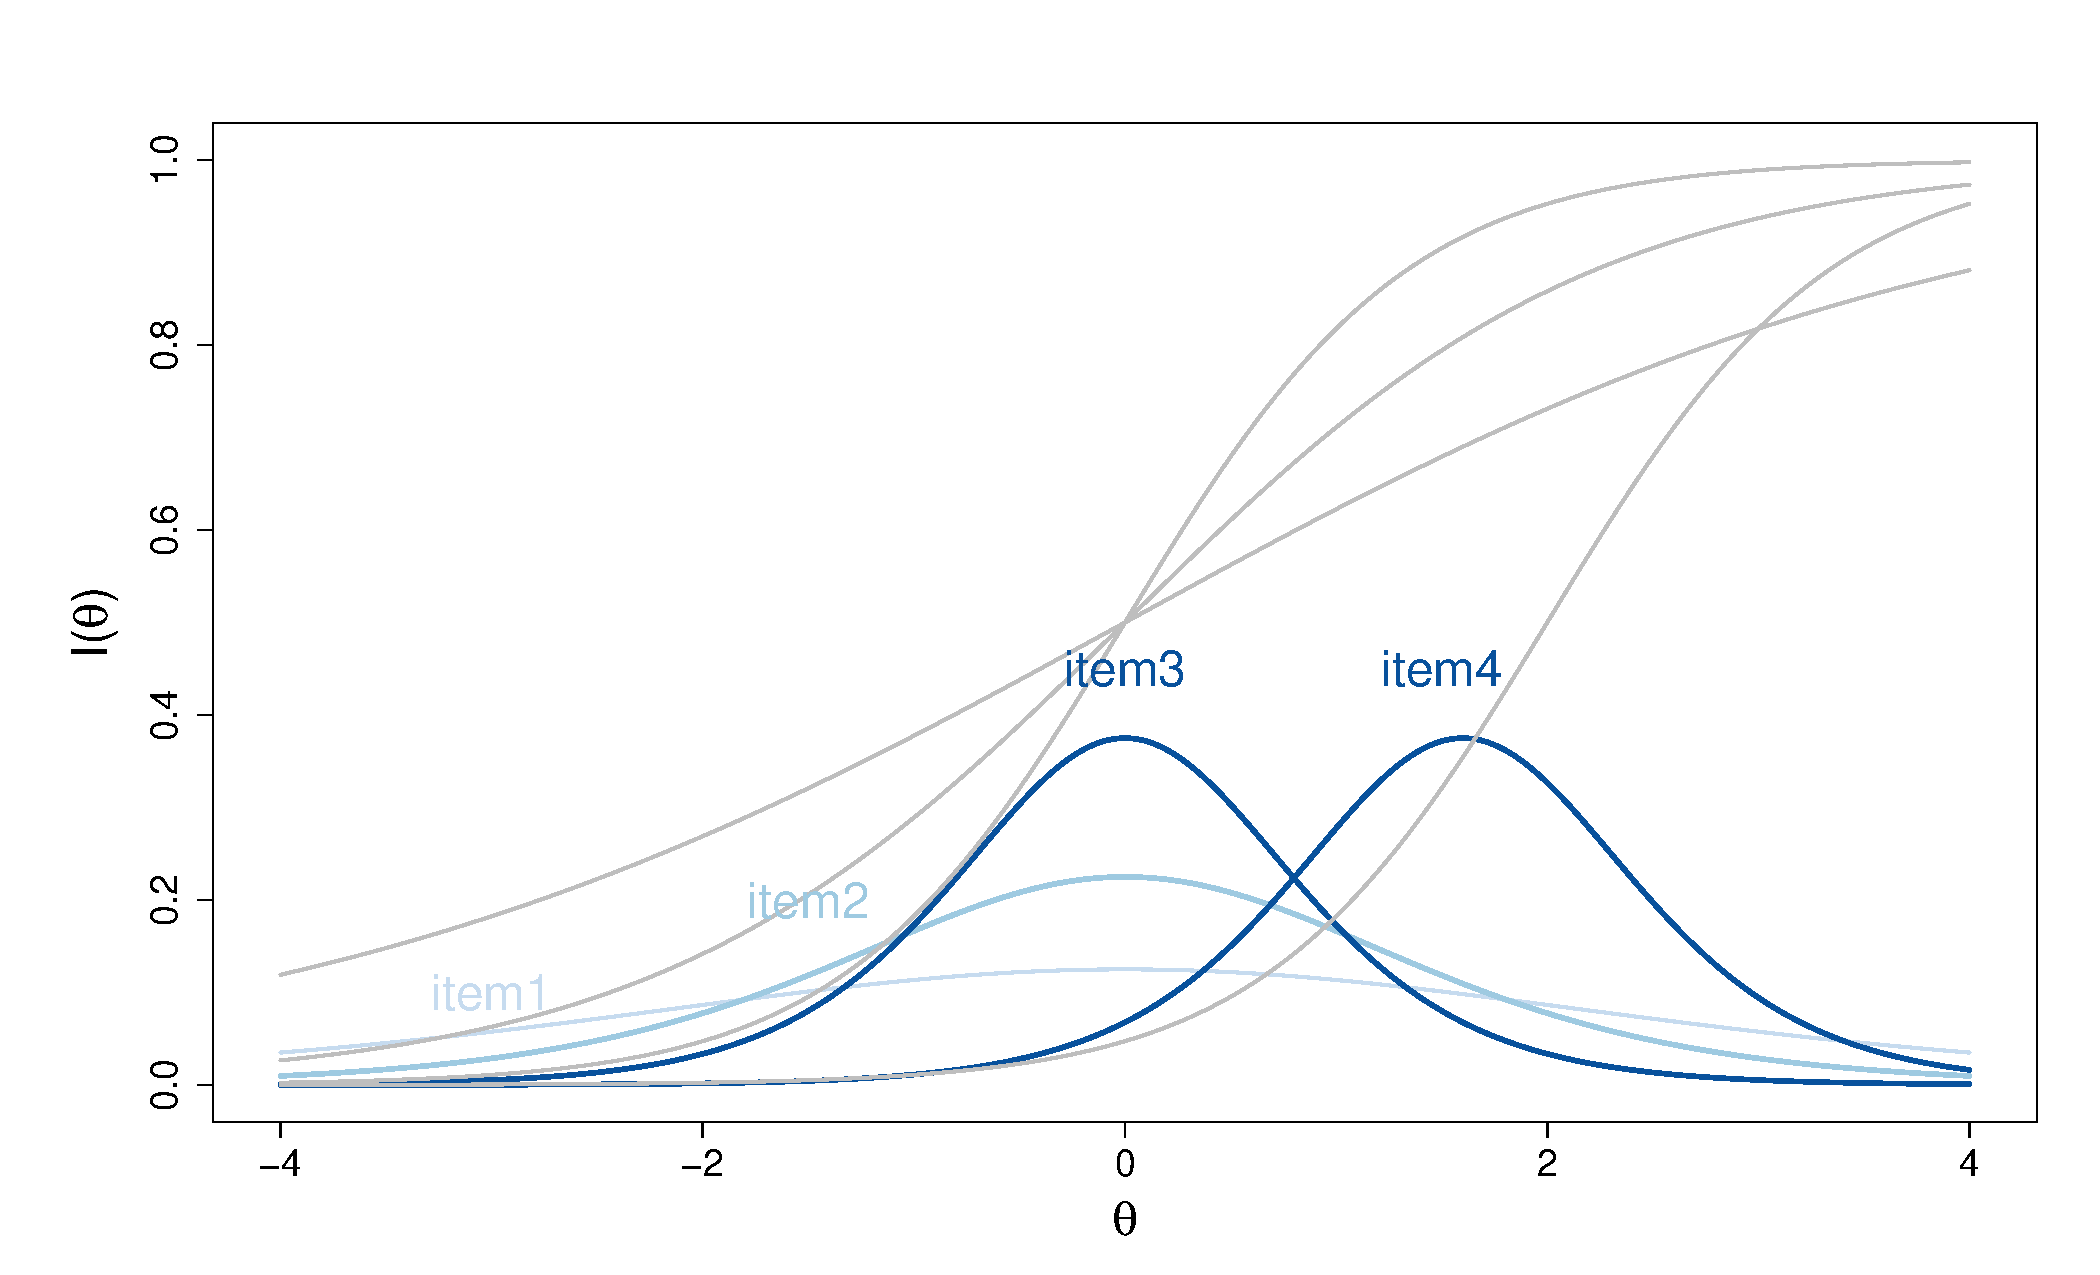
\includegraphics[width=.80\linewidth]{img/IIF-2pl.pdf}
		
		\onslide<2>
		\vspace*{3mm}
		Test Information Function:	\\	$I(\theta) =  \sum_{i = 1}^{I} I_i(\theta)$
		
		\centering
		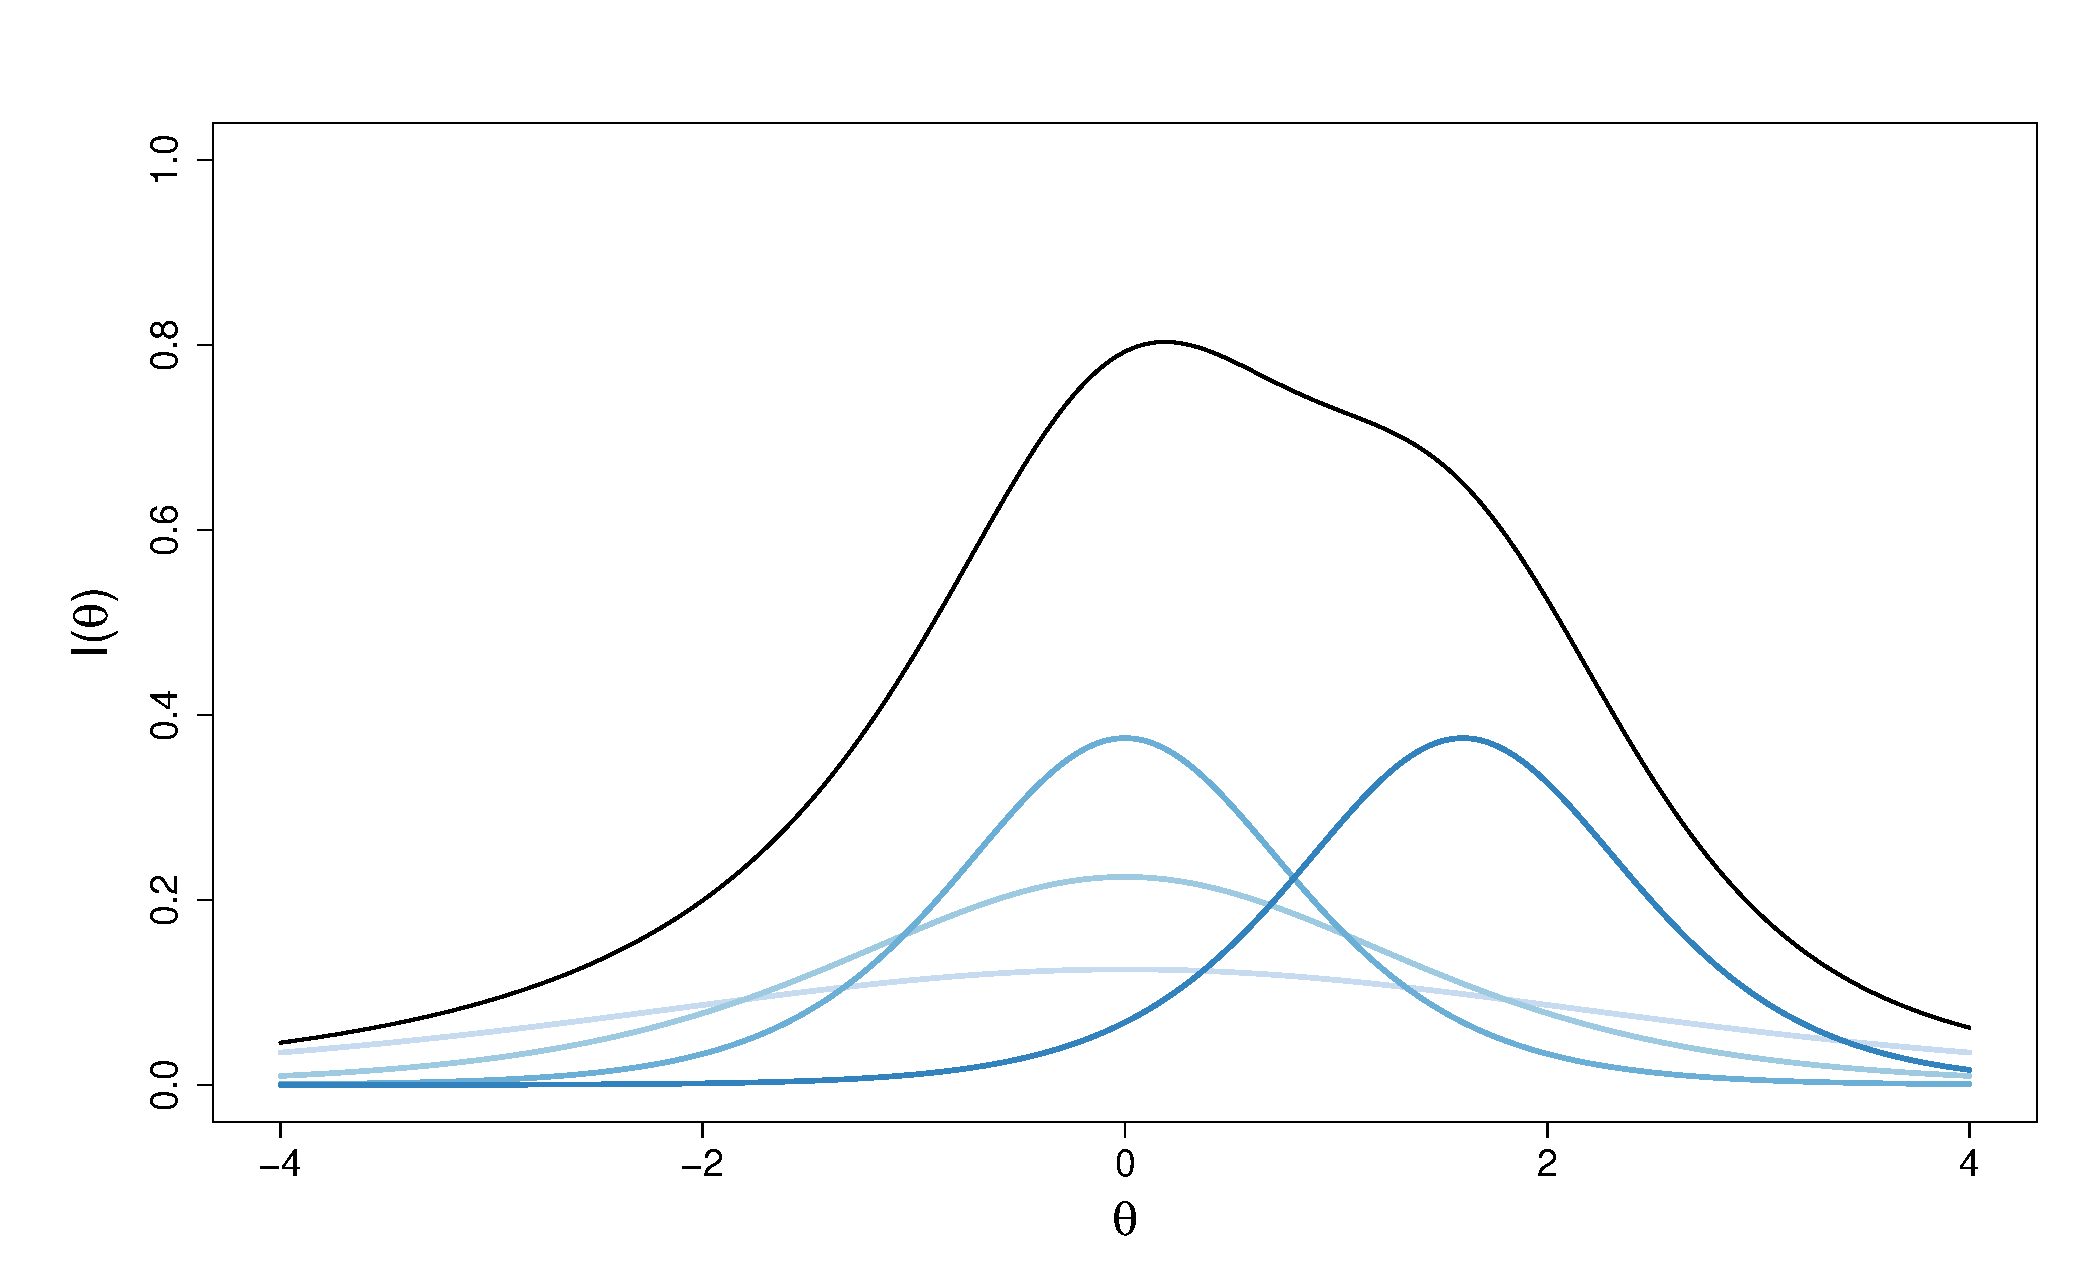
\includegraphics[width=.80\linewidth]{img/TIF-2pl.pdf}
	\end{overprint}
\end{frame}

\section[STF]{Short Test Forms}

\begin{frame}{Why?}
	Many items $\rightarrow$ good measurement precision, great reliability and so on
	
	\begin{center}
		Not always!
	\end{center}
	
	\onslide<2->
	People might get tired and frustrated 
	 
	
	\begin{block}{IRT models for the win}
		
	Being focused on the item information and on the ability of each item to measure different levels of the latent trait, IRT models provide an ideal framework for developing STF (and not torturing people)	
	\end{block}
	
\end{frame}

\begin{frame}
	
\begin{columns}[T]
	\begin{column}{.50\linewidth}
	\centering
	Static STFs
	
	\vspace{2.5mm}
	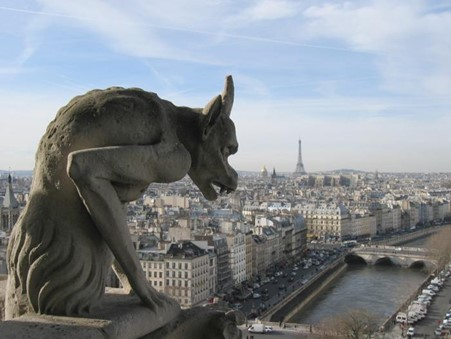
\includegraphics[width=.70\linewidth]{img/garg}	
	
	\begin{itemize}
		\small
		\color{myGreen}
		\item Equal for all respondents 
		\item Can be administered paper-and-pencil/computerized versions
		\color{unipd}
		\item Might not provide adequate measurement precision of certain regions of the latent trait
	\end{itemize}
	\end{column}
	\onslide<2->
	\begin{column}{.50\linewidth}
		\centering
		Adaptive STFs
	
	\vspace{2.5mm}
		\centering
	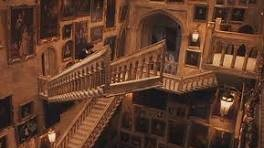
\includegraphics[width=.80\linewidth]{img/scale}	
	\begin{itemize}
		\small
		\color{myGreen}
		\item Tailored on the actual level of ability of each respondent
		\item Avoid frustration and boredom 
		\color{unipd}
		\item Fairness issues in specific evaluation contexts
	\end{itemize}
	
\end{column}

\end{columns}


\end{frame}

\section[CAT]{Computerized Adaptive Testing}

\begin{frame}
\begin{itemize}
	\item \textbf{Item bank $B$:} Entire set of items which can be administered in a CAT
	\item $||B||$: Number of items in the item bank
	\item \textbf{An item bank} \textcolor{unipd}{\textbf{must be calibrated}} 
	\item \textbf{Item calibration:} estimation of item parameters according to IRT models
\end{itemize}

\end{frame}

\begin{frame}
	
	\scalebox{.6}{
	\begin{tikzpicture}[node distance=2cm]
		
		% Nodes
		\node (start) [startstop] {Start};
		\node (ability) [process, right of=start, xshift=3cm] {Temporary Ability Estimation};
		\node (decision) [decision, below of=ability, yshift=-1.5cm] {Stopping Rule Satisfied?};
		\node (end) [startstop, below of=decision, yshift=-1.8cm] {End Administration};
		\node (final) [process, right of=end, xshift=3cm] {Final Ability estimate};
		\node (select) [process, right of=ability, xshift=3cm] {Select new items};
		\node (update) [process, above of=select, yshift=1.5cm] {Update response Pattern};
		
		% Arrows
		\draw [arrow] (start) -- (ability);
		\draw [arrow] (ability) -- (decision);
		\draw [arrow] (decision) -- node[anchor=east] {Yes} (end);
		\draw [arrow] (end) -- (final);
		
		\draw [arrow] (decision.east) -- ++(2,0) node[anchor=south, xshift=1cm] {No} -- (select);
		\draw [arrow] (select) -- (update);
		\draw [arrow] (update) -- (ability);
		
	\end{tikzpicture}
	}

\end{frame}

\section[BP]{Benchmark procedure}


\begin{frame}
	
		Create a short test form composed of $N$ items \color{template} $\rightarrow$ \normalcolor Select the $N$ items with the highest \emph{IIF}s: 
	
	\vspace{2mm}
	\begin{itemize}
		\item 	The \emph{IIF}s of the items of item bank are sorted in decreasing order: 
		
		\vspace{2mm}
		\begin{quote}
			$\mathit{iif} = (\displaystyle \max_{1 < j < J} IIF_j, \ldots \displaystyle, \min_{1 < j < J} IIF_j) $
		\end{quote}
		
		\vspace{2mm}
		\item 	Items with \emph{IIF}s from 1 to $N$, $N < J$, in \emph{iif} are selected to be included in the short test form
	\end{itemize}
\end{frame}


\begin{frame}
	
	\vspace{2mm}
	\begin{quote}
		e.g.:	3-item short form from 10-item full-length test
	\end{quote}
	\vspace*{-5mm}
	\begin{overprint}
		\onslide<1>
		\vspace{2mm}
		\begin{table}
			\begin{tabular}{l  d{3.2}d{3.2}d{3.2}}
				\toprule
				item & b_i & a_i & IIF_i \\
				\midrule
				1	& 	-0.67	 & 	0.71	 & 	0.08	\\
				2	& 	0.50	 & 	1.19	 & 	0.15	\\
				3	& 	-2.43	 & 	0.25	 & 	0.01	\\
				4	& 	2.12	 & 	1.98	 & 	0.24	\\
				5	& 	1.72	 & 	0.39	 & 	0.03	\\
				6	& 	-2.28	 & 	1.62	 & 	0.19	\\
				7	& 	0.64	 & 	0.50	 & 	0.05	\\
				8	& 	-2.51	 & 	1.68	 & 	0.19	\\
				9	& 	-0.66	 & 	0.44	 & 	0.04	\\
				10	& 	0.72	 & 	0.33	 & 	0.02	\\
				\bottomrule
			\end{tabular}
		\end{table}
		
		\onslide<2>
		\vspace{2mm}
		\begin{table}
			\begin{tabular}{l  d{3.2}d{3.2}d{3.2}}
				\toprule
				item & b_i & a_i & IIF_i \\
				\midrule
				\rowcolor{template!20!}4	& 	2.12	 & 	1.98	 & 	0.24	\\
				\rowcolor{template!20!}8	& 	-2.51	 & 	1.68	 & 	0.19	\\
				\rowcolor{template!20!}6	& 	-2.28	 & 	1.62	 & 	0.19	\\
				2	& 	0.50	 & 	1.19	 & 	0.15	\\
				1	& 	-0.67	 & 	0.71	 & 	0.08	\\
				7	& 	0.64	 & 	0.50	 & 	0.05	\\
				9	& 	-0.66	 & 	0.44	 & 	0.04	\\
				5	& 	1.72	 & 	0.39	 & 	0.03	\\
				10	& 	0.72	 & 	0.33	 & 	0.02	\\
				3	& 	-2.43	 & 	0.25	 & 	0.01	\\
				\bottomrule
				
			\end{tabular}
		\end{table}
		
	\end{overprint}
	
	
	
\end{frame}



%\section{$\theta$-Target Procedure}
%
%\begin{frame}{$\theta$-target procedures}
%	Selected items $\rightarrow$ items with highest \emph{IIF}s in respect to $\theta$ targets ($\theta'$) 
%	
%	\begin{quote}
%		e.g.:	3-item short form from 10-item full-length test
%	\end{quote}
%	\vspace*{-5mm}
%	\begin{overprint}
%		\onslide<1>
%		\begin{table}
%			\small
%			\begin{tabular}{l l l l }
%				\toprule
%				& \multicolumn{1}{c}{$\theta_1'$} & \multicolumn{1}{c}{$\theta_2'$} & \multicolumn{1}{c}{ $\theta_3'$} \\
%				item	& $	-2.67	$ & $	0.01	$ & $	2.67	$ \\
%				\midrule
%				1	& & & \\
%				2	&  & & 	\\
%				3	&  &  &  \\
%				4&  & & \\
%				5	&  & & 	 \\
%				6	&  & &  \\
%				7	& & &  \\
%				8	& & &  \\
%				9	& &  &  \\
%				10	&& & 	 \\
%				\bottomrule
%			\end{tabular}
%		\end{table}
%		\onslide<2->
%		\begin{table}
%				\small
%			\begin{tabular}{l l l l }
%				\toprule
%				& \multicolumn{1}{c}{\textcolor<3->{orangered2}{$\theta_1'$}} & \multicolumn{1}{c}{\textcolor<7->{springgreen}{$\theta_2'$}} & \multicolumn{1}{c}{ \textcolor<5->{diff}{$\theta_3'$}} \\
%				item	& \textcolor<3->{orangered2}{$	-2.67	$} & \textcolor<7->{springgreen}{$	0.01	$} & \textcolor<5->{diff}{$	2.67	$} \\
%				\midrule
%				1	& \textcolor<4->{black!30}{$	0.04	$} & \textcolor<8->{black!30}{$	0.12	$} & 	\textcolor<6->{black!30}{$	0.08	$} \\
%				\textcolor<8->{black!30 }{2}	& \textcolor<4->{black!30}{$	0.09	$} & \textcolor<7->{springgreen}{$	0.33	$} & 	\textcolor<6->{black!30}{$	0.03	$} \\
%				3	& \textcolor<4->{black!30}{$	0.01	$} & \textcolor<8->{black!30}{$	0.01	$} & 	\textcolor<6->{black!30}{$	0.02	$} \\
%				\textcolor<4->{black!30}{4}	& \textcolor<3->{orangered2}{$	0.73	$} & \textcolor<4->{black!30}{$	0.06	$} & \textcolor<4->{black!30}{$	0.01	$} \\
%				5	& \textcolor<4->{black!30}{$	0.04	$} & \textcolor<8->{black!30}{$	0.03	$} & 	\textcolor<6->{black!30}{$	0.02	$} \\
%				6	& \textcolor<4->{black!30}{$	0.01	$} & \textcolor<8->{black!30}{$	0.06	$} & 	\textcolor<6->{black!30}{$	0.59	$} \\
%				7	& \textcolor<4->{black!30}{$	0.05	$} & \textcolor<8->{black!30}{$	0.06	$} & 	\textcolor<6->{black!30}{$	0.03	$} \\
%				\textcolor<6->{black!30}{8}	& \textcolor<4->{black!30}{$	0.01	$} & 	\textcolor<6->{black!30}{$	0.04	$} & \textcolor<5->{diff}{$	0.69	$} \\
%				9	& \textcolor<4->{black!30}{$	0.03	$} & \textcolor<8->{black!30}{$	0.05	$} & 	\textcolor<6->{black!30}{$	0.04	$} \\
%				10	& \textcolor<4->{black!30}{$	0.02	$} & \textcolor<8->{black!30}{$	0.03	$} & 	\textcolor<6->{black!30}{$	0.02	$} \\
%				\bottomrule
%			\end{tabular}
%		\end{table}
%		
%	\end{overprint}
%	
%	
%	
%\end{frame}

\section[$\theta$-target]{$\theta$-target Procedure}

\begin{frame}{Procedures based on $\theta$ targets}
	
	Create a short test form composed of $N$ items:
	
	\vspace{1.5mm}
	\begin{itemize}
		\item Define $N$ trait levels of interest \color{template} 
		$\rightarrow$ \normalcolor $\theta$ targets ($\theta'$s)
		
		
		\vspace{1.5mm}
		\item Choose the items that most precisely assess the identified $\theta's$
		
	\end{itemize}
\end{frame}


\begin{frame}
	\vspace*{-1mm}
	\small
	$\mathbf{IIF}^{J\times N}$: Matrix of items information functions $\mathit{iif}_{jn}$:
	\vspace*{-1mm}
	\begin{center}
		\begin{tabular}{p{0.7cm}  p{0.7cm}  |p{0.7cm}  p{0.7cm} p{0.7cm} p{0.7cm} p{0.7cm} p{0.7cm} | p{0.7cm}}
			& \multicolumn{1}{l}{} & \multicolumn{6}{c}{$\theta'$} & \multicolumn{1}{c}{} \\
			& \multicolumn{1}{c}{} & \multicolumn{1}{l}{1} & \multicolumn{1}{l}{2} & \multicolumn{1}{l}{$\ldots$} & 
			\multicolumn{1}{l}{$n$} & \multicolumn{1}{l}{$\ldots$} & \multicolumn{1}{l}{$N$}& \multicolumn{1}{l}{} \\
			\cline{3-8}
			\multirow{8}{*}{Items} & 1 & $\mathit{iif}_{11}$ & $iif_{12}$ & & &  &  &  \\
			&	2& $\mathit{iif}_{21}$ & $\mathit{iif}_{22}$ & & $\vdots$ & &  &  \\
			&	$\vdots$ &  &  &  & $\vdots$   &  &  & \\
			&\emph{j}& $\ldots$ & $\ldots$ & $\ldots$ & $\mathit{iif}_{jn}$ & $\ldots$ & $\ldots$ &  \\
			&$\vdots$	&  &  &  & $\vdots$   &  &  &  \\
			&	\emph{J} &  &  & & $\vdots$ &  & $\mathit{iif}_{JN}$ &  \multicolumn{1}{c}{}\\
			\cline{3-8}
		\end{tabular}
	\end{center}
	$j = 1, \ldots, J$: Items in the item bank $B$ composed of $||B|| = J$ items;\\
	$n = 1, \ldots, N$: Items to be included in the $N$-item short test form (selected according to the $N$ $\theta$ targets, $\theta'$s);\\	
\end{frame}

\begin{frame}
	
	\small
	$k = 0, \ldots, K$: Scalar denoting the iterations of the procedures ($K = N-1$);\\ 
	$S^k \subseteq \{1, \ldots J\}$: Set of items selected to be included in the short test form up to iteration $k$.\\
	$Q^k \subseteq \{1, \ldots N\}$: Set of $\theta'$s satisfied up to iteration $k$;\\
	
	\vspace{1.5mm}
	\pause
	At $k=0$: 
	
	\vspace{1.5mm}
	\begin{itemize}
		\item $S^0 = \emptyset$
		\item $Q^0 = \emptyset$
	\end{itemize}
	
	The procedure cycles steps 1 to 3 until $k = K$:
	
	\begin{enumerate}
		\item Select $iif_{jn}^k = \displaystyle  \max_{j \in J\setminus S^k, \, n  \in N \setminus Q^k} \mathbf{IIF}(j,n)$;
		\item Compute $S^{k+1} = S^k \cup \{j\}$ as the set of item(s) selected at $k$; 
		\item Compute $Q^{k+1} = Q^k \cup \{n\}$ as the set of $\theta'$s satisfied at $k$; 
	\end{enumerate}
	\vspace{1.5mm}
	
	At iteration $K$, $|Q^{K + 1}| = N$ and   $|S^{K + 1}| = N$ 
	
\end{frame}

\begin{frame}{$k=0$}
	
	\vspace*{-4mm}
	\begin{overprint}
		\small
		\onslide<1>
		\begin{equation*}
			\mathbf{IIF} =
			\left[\begin{array}{c>{\columncolor{template!20}}c>{\columncolor{template!20}}c>{\columncolor{template!20}}cc}
				&0.12	  & 	0.12	  & 	0.09 & \\
				&0.14	  & 	0.32	  & 	0.31 &\\
				&0.02	  & 	0.01	  & 	0.01 &\\
				&0.01	  & 	0.05	  & 	0.43&\\
				&0.03	  & 	0.03	  & 	0.04&\\
				&0.35	  & 	0.07	  & 	0.01&\\
				&0.05	  & 	0.06	  & 	0.06&\\
				&0.27	  & 	0.04	  & 	0.01&\\
				&0.05	  & 	0.05	  & 	0.04&\\
				&0.02	  & 	0.03	  & 	0.03 &\\
			\end{array}\right]
		\end{equation*}
		\onslide<2->
		\small
		\begin{equation*}
			\mathbf{IIF} =
			\left[\begin{array}{c>{\columncolor{template!20}}c>{\columncolor{template!20}}c>{\columncolor{template!20}}cc}
				&0.12	  & 	0.12	  & 	0.09 & \\
				&0.14	  & 	0.32	  & 	0.31 &\\
				&0.02	  & 	0.01	  & 	0.01 &\\
				&0.01	  & 	0.05	  & 	\mathbf{0.43}&\\
				&0.03	  & 	0.03	  & 	0.04&\\
				&0.35	  & 	0.07	  & 	0.01&\\
				&0.05	  & 	0.06	  & 	0.06&\\
				&0.27	  & 	0.04	  & 	0.01&\\
				&0.05	  & 	0.05	  & 	0.04&\\
				&0.02	  & 	0.03	  & 	0.03 &\\
			\end{array}\right]
		\end{equation*}
	\end{overprint}
	
	\vspace{2mm}
	\small
	\onslide<2->
	$\mathit{iif}_{\text{max}}^0=\displaystyle \max_{j \in J\setminus S^0, \, n  \in N \setminus Q^0} \mathbf{IIF}= \mathbf{IIF}(4,3) = 0.43$\\
	\onslide<2-> \vspace{1.5mm}
	$S^{1} = S^0 \cup \{4\}$ = \{4\}\\ \vspace{1.5mm}
	$Q^{1} = Q^0 \cup \{3\}$ = \{3\}\\ 
	
\end{frame}

\begin{frame}{$k=1$}
	\vspace*{-4mm}
	\small
	\begin{equation*}
		\mathbf{IIF} =
		\left[\begin{array}{ccccc}
			&\high 0.12	  & 	\high 0.12	  & 	0.09 & \\
			&\high0.14	  & 	\high 0.32	  & 	0.31 &\\
			&\high0.02	  & 	\high 0.01	  & 	0.01 &\\
			&0.01	  &   0.05	  & 	0.43&\\
			&\high0.03	  & \high	0.03	  & 	0.04&\\
			&\high\mathbf{0.35}	  & \high	0.07	  & 	0.01&\\
			&\high0.05	  & 	\high0.06	  & 	0.06&\\
			&\high0.27	  & 	\high0.04	  & 	0.01&\\
			&\high0.05	  & 	\high0.05	  & 	0.04&\\
			&\high0.02	  & 	\high0.03	  & 	0.03 &\\
		\end{array}\right]
	\end{equation*}
	\vspace{2mm}
	$\mathit{iif}_{max}^1=\displaystyle \max_{j \in J\setminus S^1, \, n  \in N \setminus Q^1}  \mathbf{IIF} = \mathbf{IIF}(6,1)= 0.35$\\ \vspace{1.5mm}
	$S^{2} = S^1 \cup \{6\} = \{4, 6\}$\\ \vspace{1.5mm}
	$Q^{2} = Q^1 \cup \{1\} = \{3, 1\}$\\ 
\end{frame}


\begin{frame}{$k=2$}
	\vspace*{-4mm}
	\small
	\begin{equation*}
		\mathbf{IIF} =
		\left[\begin{array}{ccccc}
			&0.12	  & \high	0.12	  & 	0.09 & \\
			&0.14	  & 	\high \mathbf{0.32}	  & 	0.31 &\\
			&0.02	  & 	\high 0.01	  & 	0.01 &\\
			&0.01	  & 	0.05	  & 	0.43&\\
			&0.03	  & 	\high0.03	  & 	0.04&\\
			&0.35	  & 	0.07	  & 	0.01&\\
			&0.05	  & 	\high0.06	  & 	0.06&\\
			&0.27	  & 	\high0.04	  & 	0.01&\\
			&0.05	  & 	\high0.05	  & 	0.04&\\
			&0.02	  & 	\high0.03	  & 	0.03 &\\
		\end{array}\right]
	\end{equation*}
	\vspace{1.5mm}
	$\mathit{iif}_{max}^2=\displaystyle \max_{j \in J\setminus S^2, \, n  \in N \setminus Q^2} \mathbf{IIF} = \mathbf{IIF}(2,2) = 0.32$\\ \vspace{1.5mm}
	
			$S^{3} = S^2 \cup \{2\} = \{4, 6, 2\}$\\ \vspace{1.5mm}
			$Q^{3} = Q^2 \cup \{2\} = \{3,1, 2\}$\\ \vspace{1.5mm}
			
			\pause
			$|S^3| = 3$,   \hspace{3mm} $|Q^3| = 3$, $K = 2$ $\rightarrow$ \texttt{end}
\end{frame}

\begin{frame}
	\vspace*{-3mm}
	\begin{overprint}
		\onslide<1>
		\begin{figure}
			\centering
			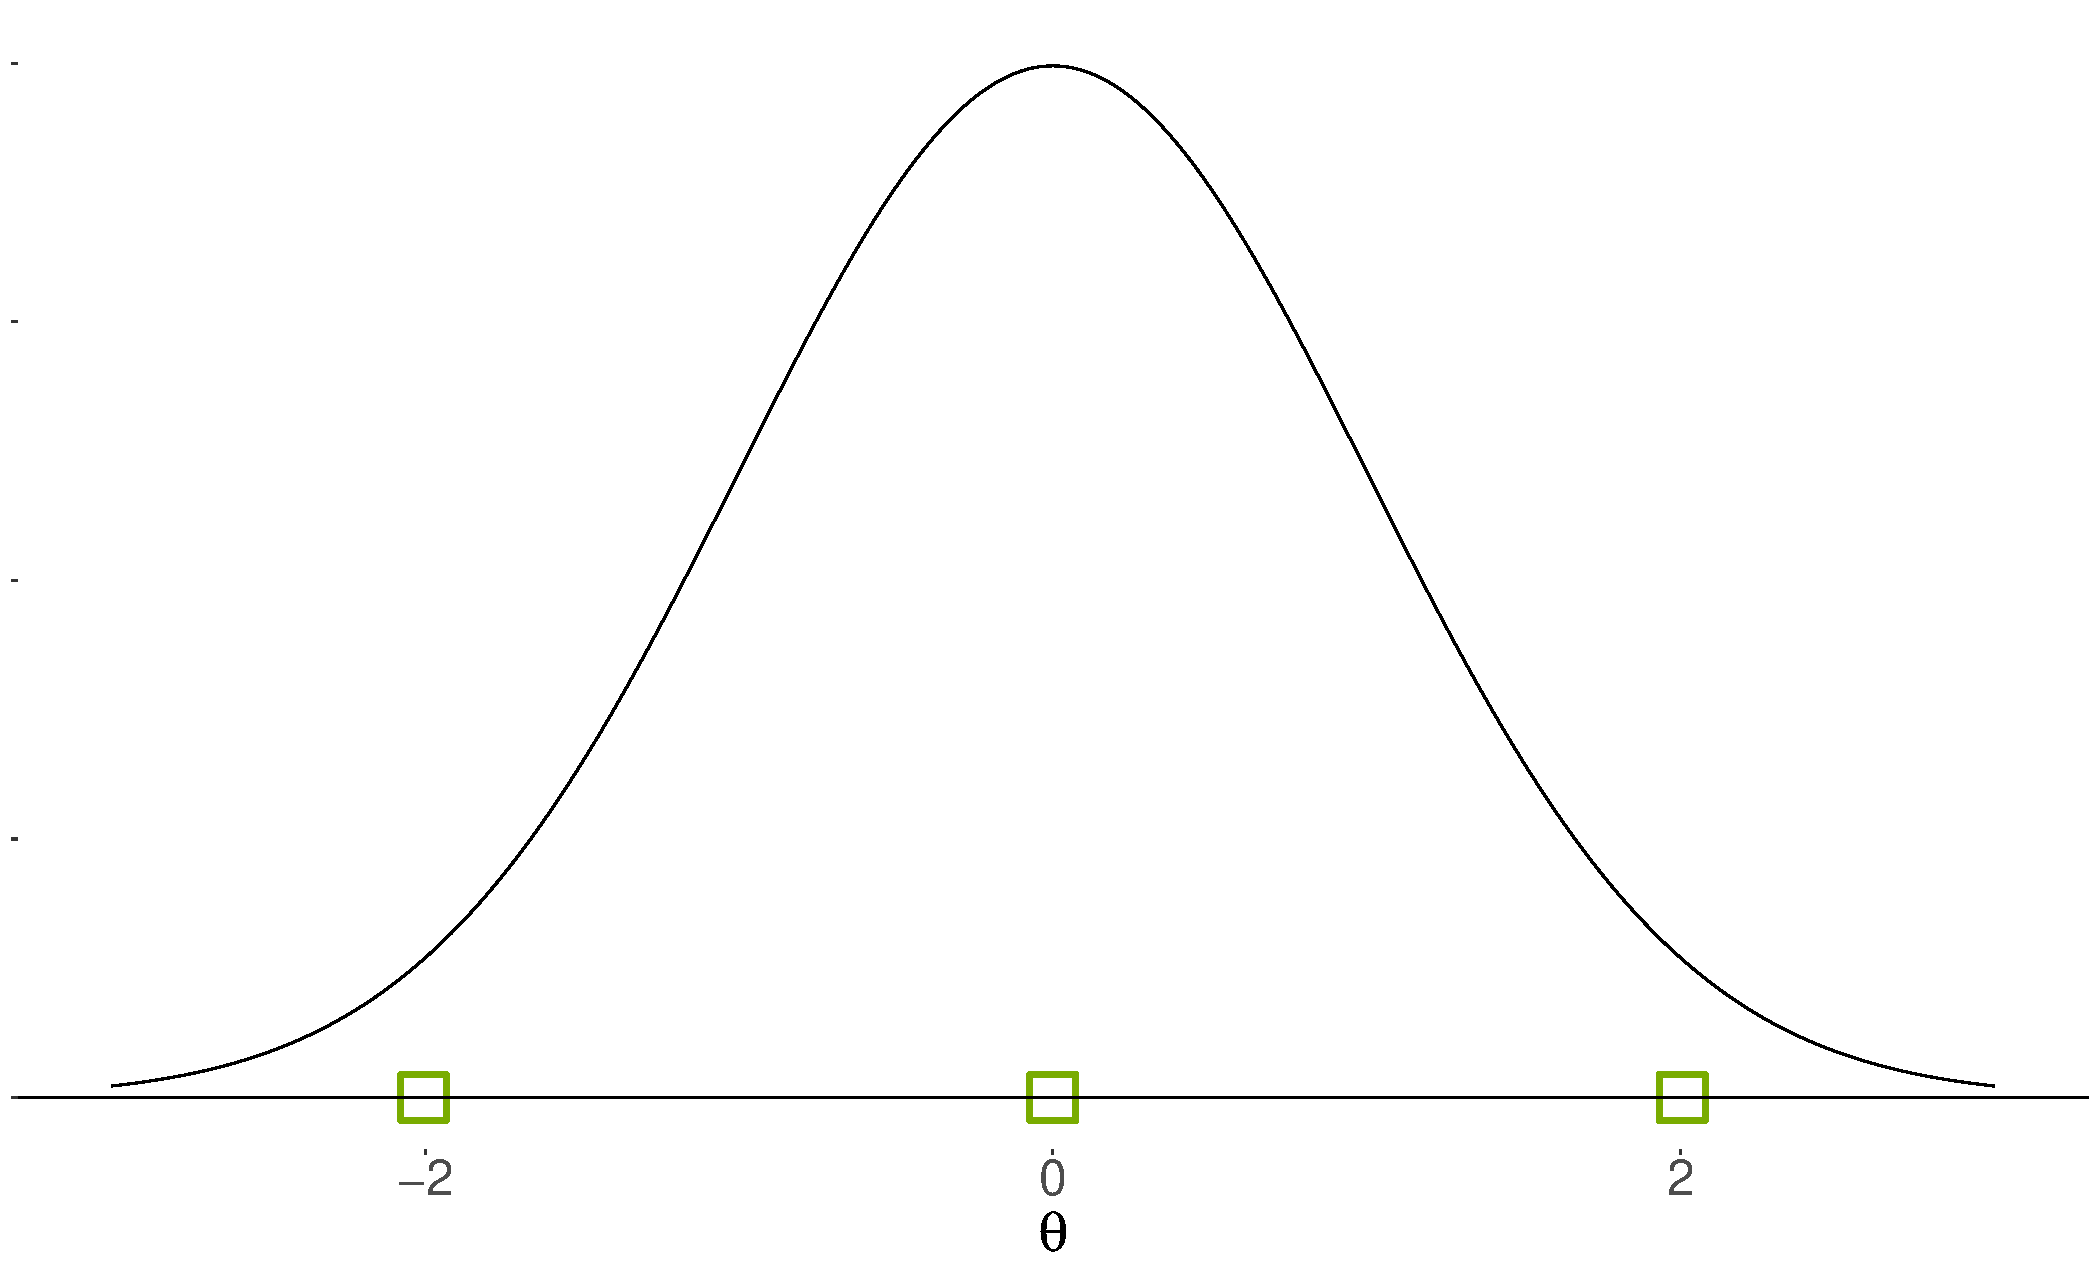
\includegraphics[width=.50\linewidth]{img/eip}
		\end{figure}
		\onslide<2>
		\begin{figure}
			\centering
			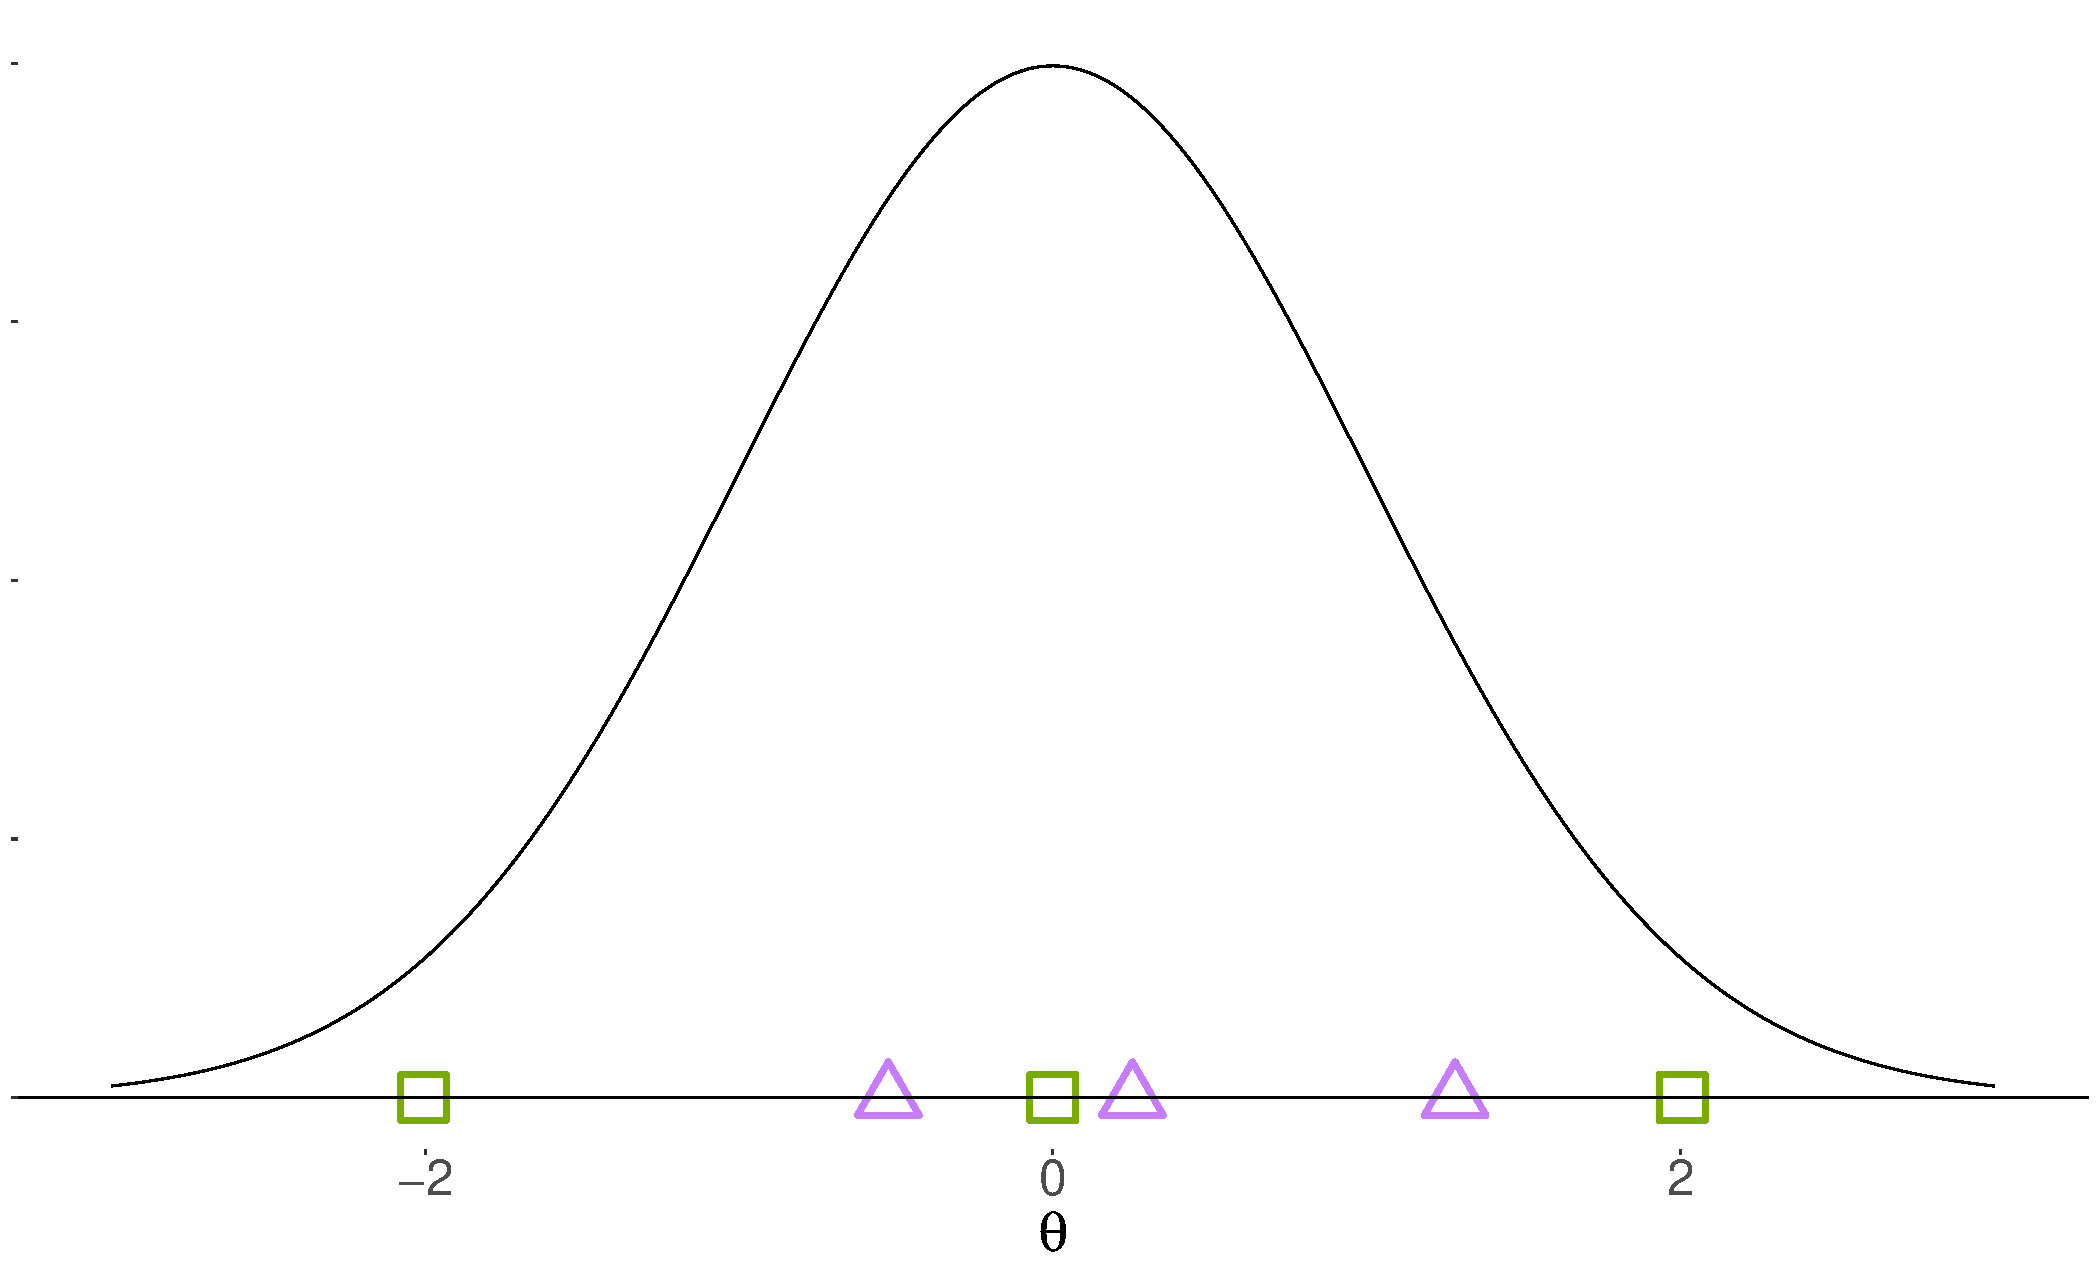
\includegraphics[width=.50\linewidth]{img/latent}
		\end{figure}
	\end{overprint}
	\begin{columns}[T]
		\begin{column}{.50\linewidth}
			\begin{center}
				\small
				\textbf{\textcolor{eip}{Equal Intervals Procedure (EIP)}}
			\end{center} \small	Segmentation in $N + 1$ intervals of width $w = (\theta_{max} - \theta_{min}) / N$ \\
			\vspace{2mm}
			Each interval: $[\theta_{n-1}; \,\theta_{n}]$ \\
			\vspace{2mm}
			$\theta_n' = (\theta_{n-1} + \theta_{n})/2$ 
			
		\end{column}
		\onslide<2->
		\begin{column}{.50\linewidth}
			
			\begin{center}
				\small
				\textbf{\textcolor{uip}{Unequal Intervals Procedure (UIP)}} 
			\end{center}
			
			\small
			Clustering in $N$ clusters  	
			
			\vspace{2mm}
			The $c_n$ centroids are the $\theta'$s
		\end{column}
	\end{columns}
	
\end{frame}

%\section{Comparison}

\begin{frame}
	Comparison between the item selection procedures: 
	\begin{itemize}
		\item \textbf{\textcolor{bp}{Benchmark procedure (BP)}}: The $N$ items with the highest \emph{IIF}s are selected from the full-length test
		\item \textbf{\textcolor{eip}{Equal Intervals Procedure (EIP)}}: The $N$ items that maximize the information for each $\theta'$ obtained by dividing the latent trait into equal intervals are selected
		\item \textbf{\textcolor{uip}{Unequal Intervals Procedure (UIP)}}:  The $N$ items that maximize the information for each $\theta'$ obtained by clustering the latent trait are selected 
		
		\item \textbf{\textcolor{rp}{Random Procedure (RP)}}: $N$ items are randomly selected from the full-length tests 
	\end{itemize}
	\vspace{3mm}
	10, 30, 50, 70, 90-item short test forms from a  100-item full-length test 
	
\end{frame}



\begin{frame}

			\begin{center}
				\textbf{1000 respondents $p$:}
			\end{center}
			\begin{enumerate}
				\item Normal distribution: $p \sim \mathcal{N}(0,1)$
				\item Positive skewed distribution: $p \sim Beta(1, 100)$ \tiny(linearly transformed to obtain negative values)
				\normalsize
				\item Uniform distribution: $p \sim \mathcal{U}(-3,3)$
			\end{enumerate}
			
			\vspace{3mm}
			\begin{center}
			\textbf{	100 items $i$:}
			\end{center}
			\begin{itemize}
				\item $b \sim \mathcal{U}(-3,3)$
				\item  $a \sim \mathcal{U}(0.40,2)$
			\end{itemize}
\end{frame}


\begin{frame}
	\begin{figure}
		\centering
		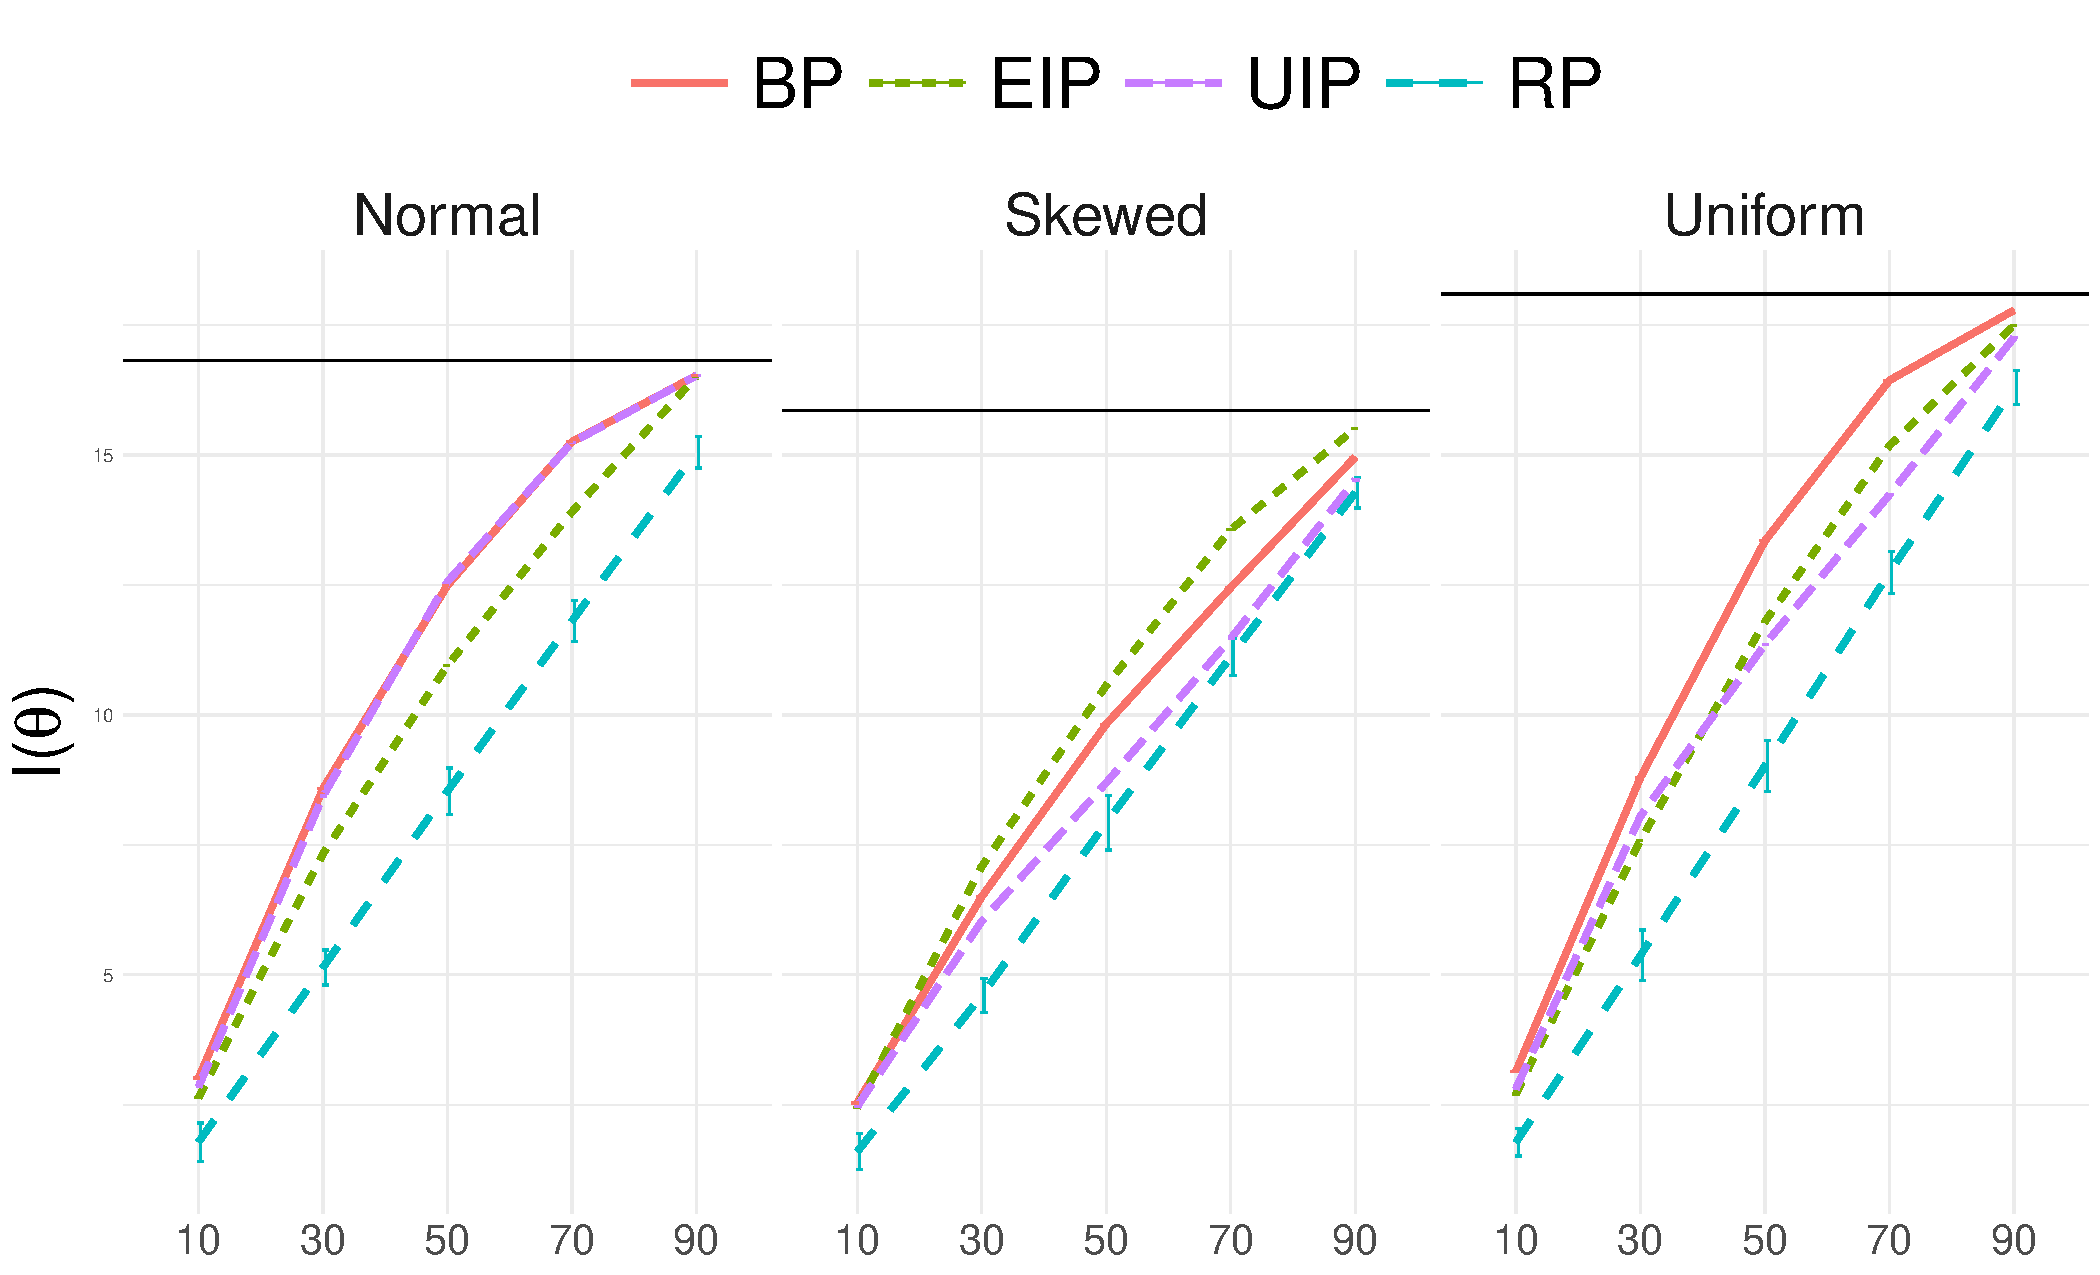
\includegraphics[width=.80\linewidth]{img/info.pdf}
		\caption{Overall Information of the short test forms}
	\end{figure}
\end{frame}


\begin{frame}
	\begin{figure}
		\centering
		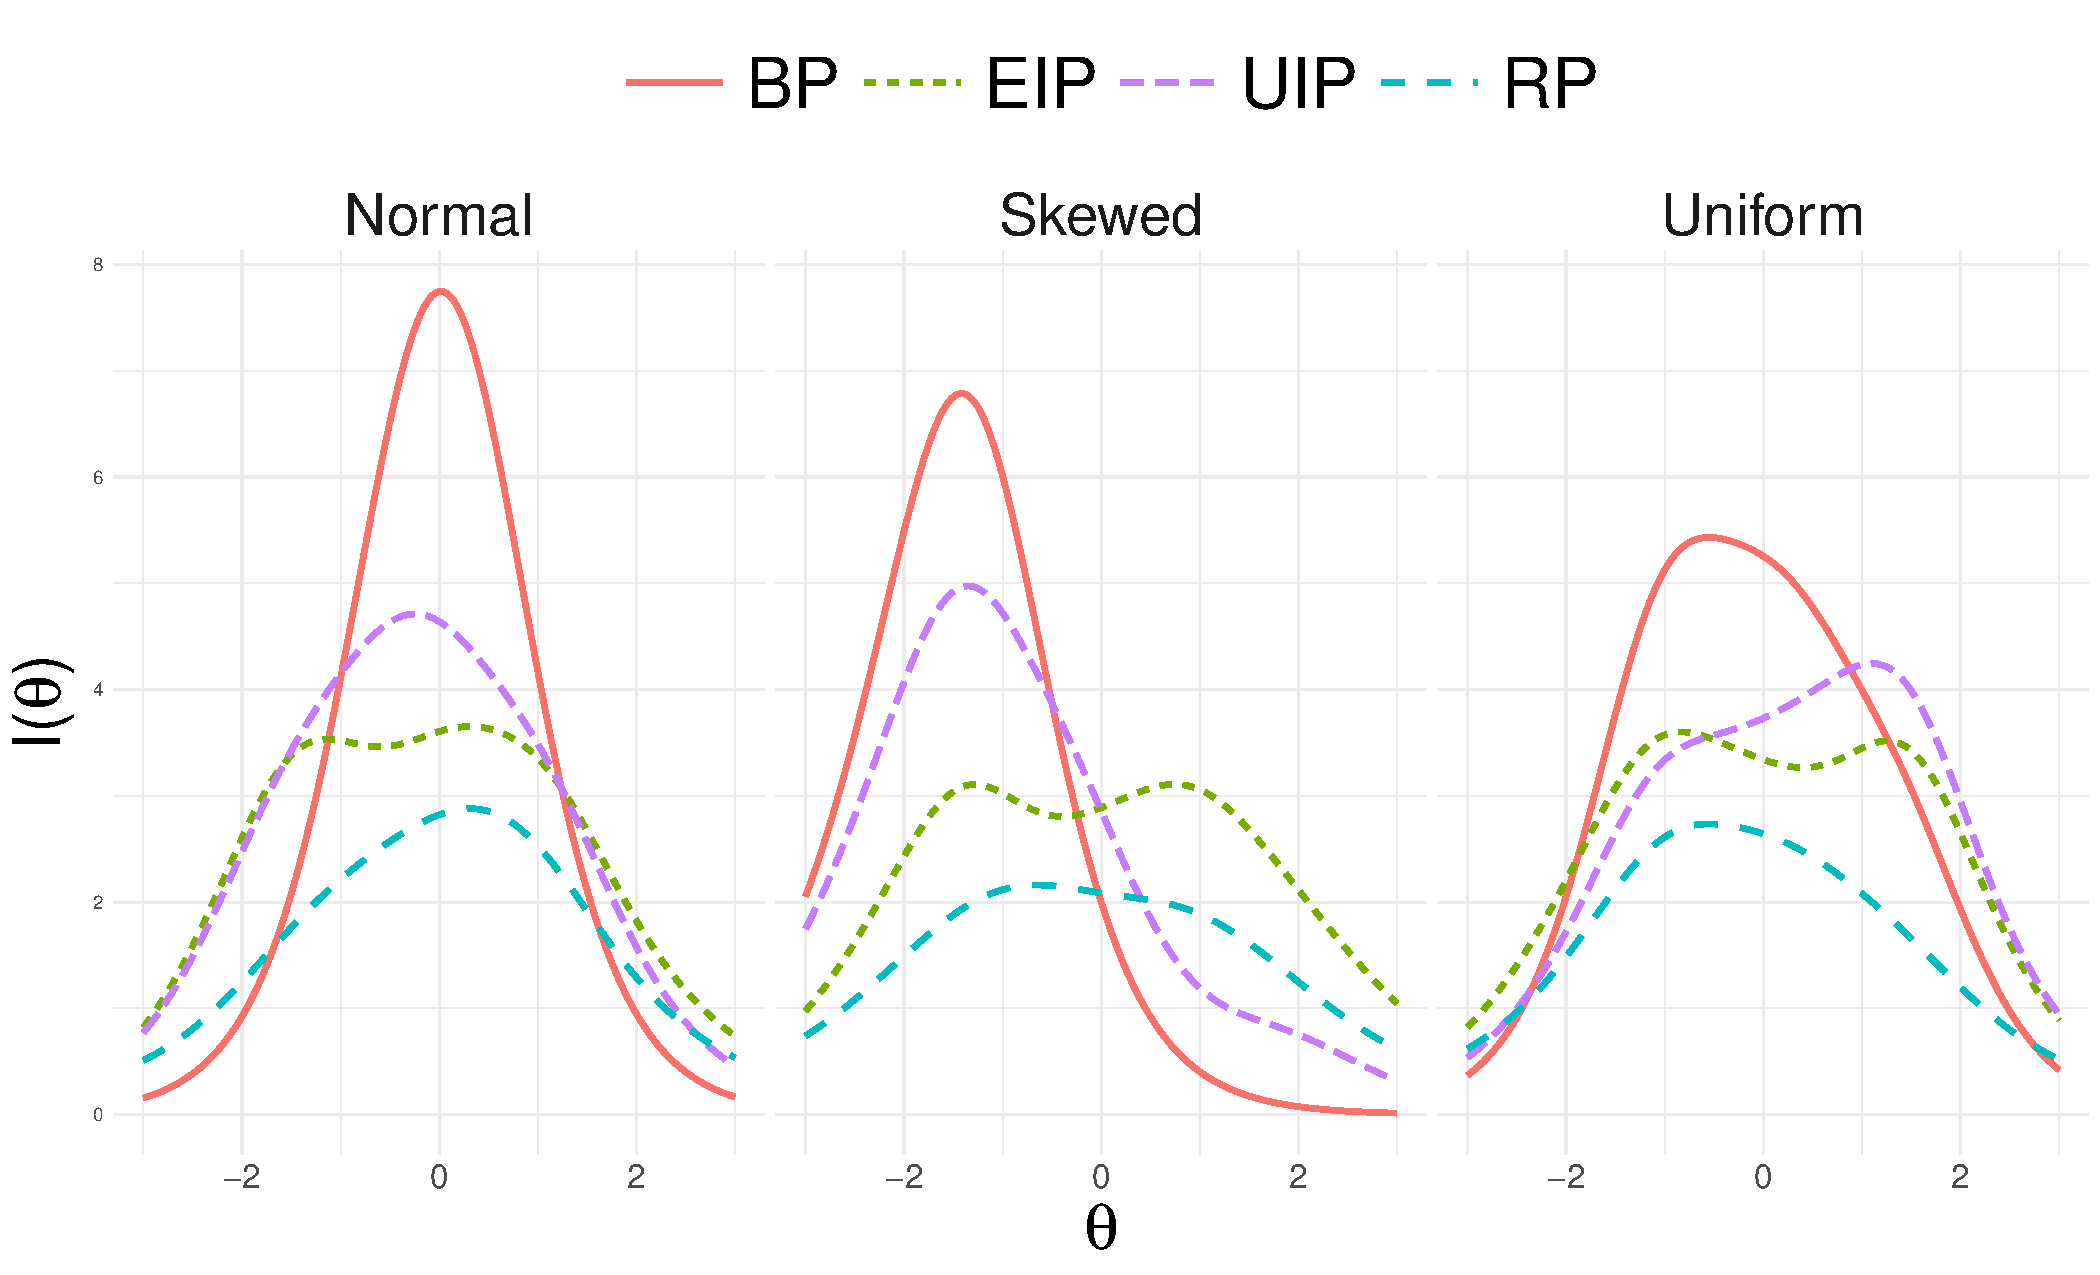
\includegraphics[width=.80\linewidth]{img/infoDetails.pdf}
		\caption{TIF of the 10-item short test form}
	\end{figure}
\end{frame}

\begin{frame}
	\begin{figure}
		\centering
		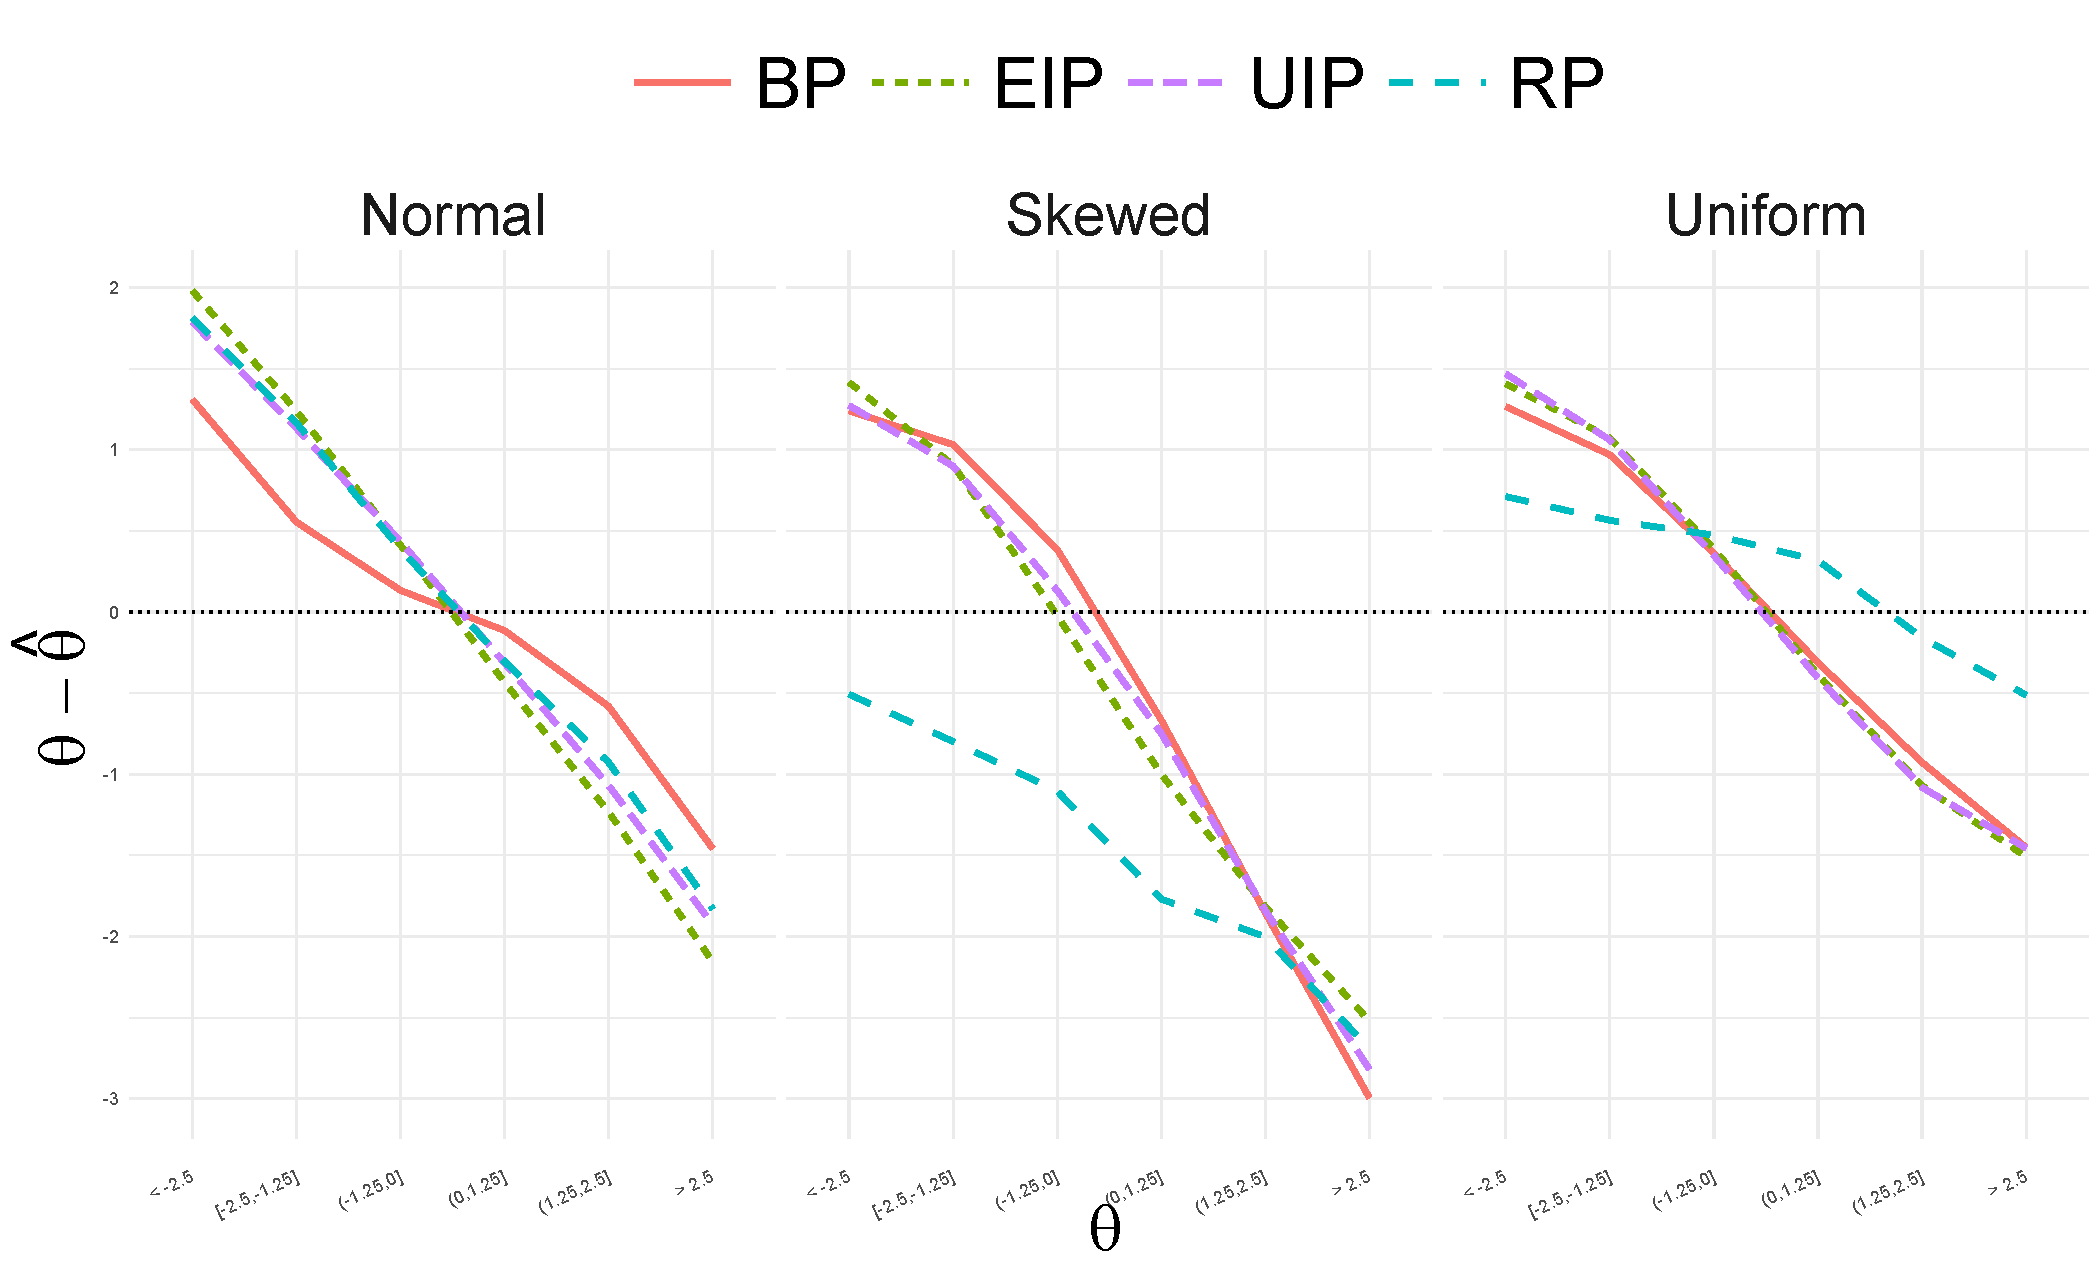
\includegraphics[width=.80\linewidth]{img/BIAS.pdf}
		\caption{$bias = \theta - \hat{\theta}$ of the 10-item short test form}
	\end{figure}
\end{frame}

\begin{frame}


\begin{exampleblock}{Good!}
	
	There's no ``one-fits-all'' solution
	
	\vspace{2mm}
	
	The $\theta$ distribution is a key element
\end{exampleblock}

\pause
\begin{alertblock}{..but work is still needed}
	
	Lack of direct comparison with CAT
	
	Real life applications are missing
	
	The number of items included in the STF strictly depends on the $\theta$ targets $\rightarrow$ One item for each target
	
\end{alertblock}

\end{frame}

\section[\texttt{shortIRT}]{The \texttt{shortIRT} package}

\begin{frame}[plain]{The \texttt{shortIRT} package}
\begin{figure}
	\centering
	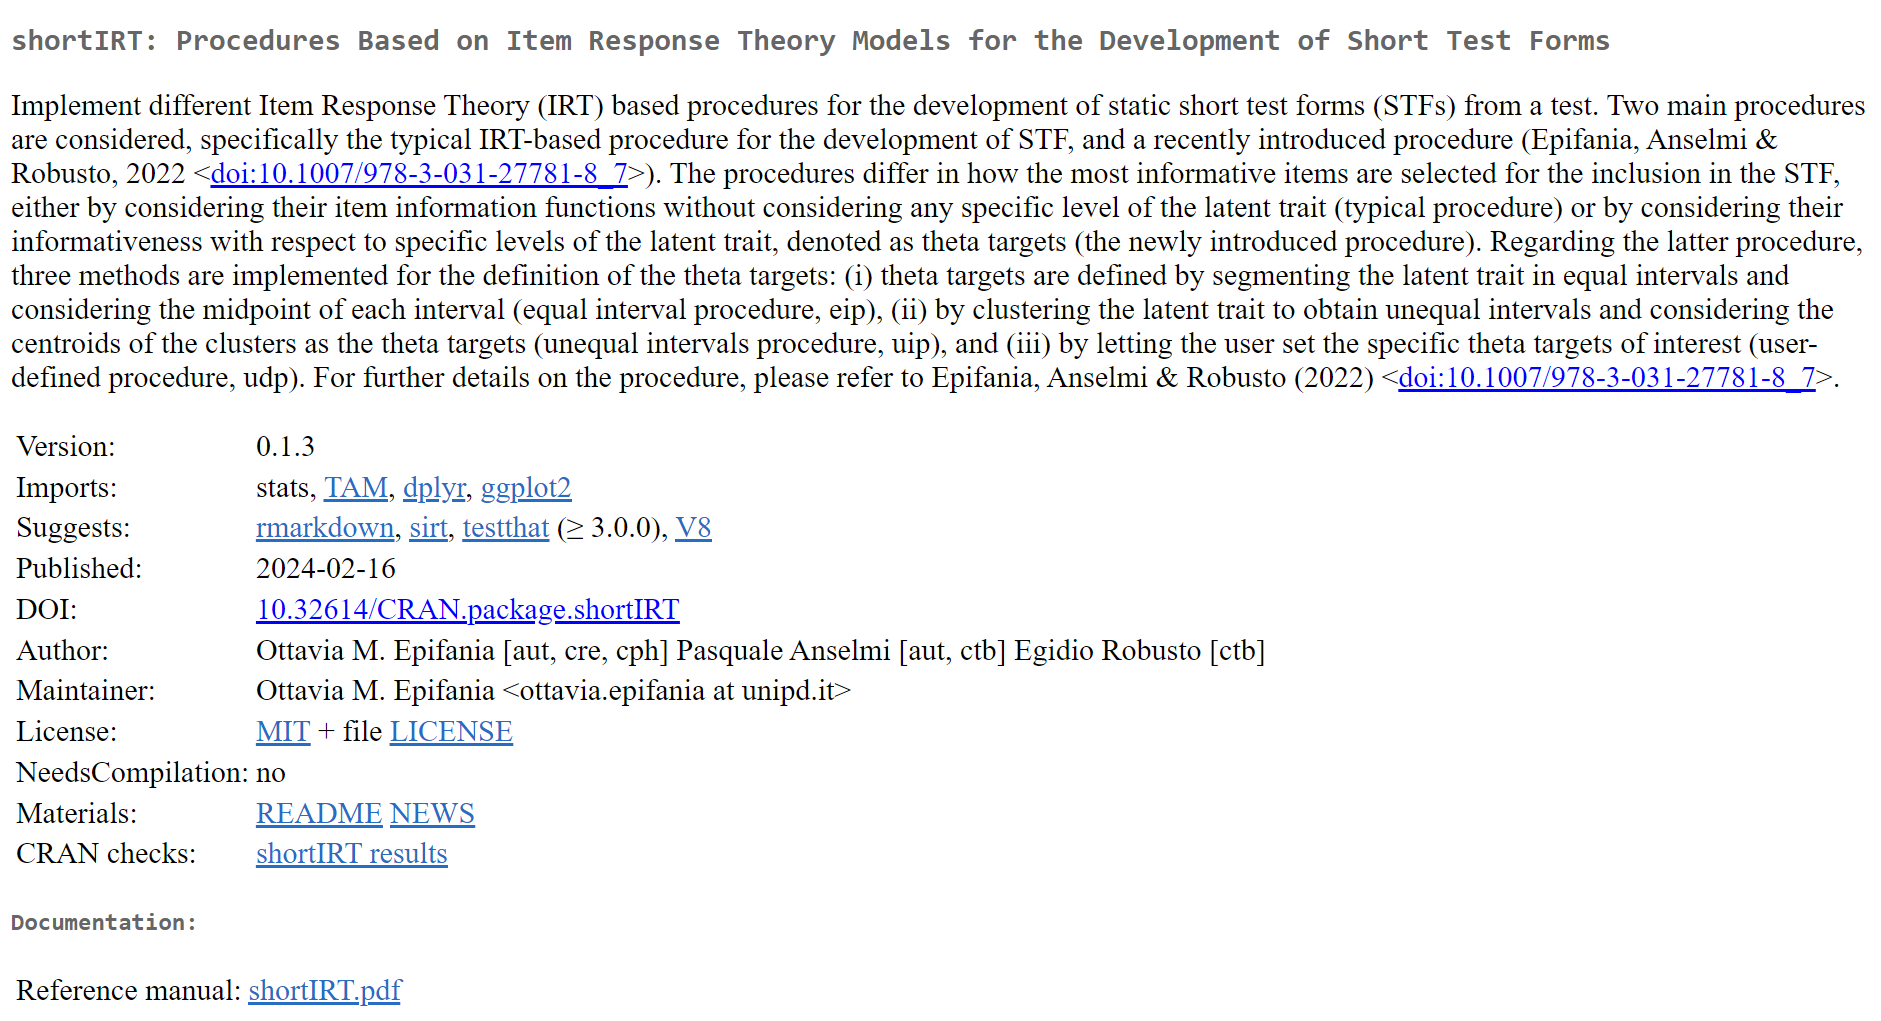
\includegraphics[width=\linewidth]{img/shortIRT}
\end{figure}

\href{https://cran.r-project.org/web/packages/shortIRT/index.html}{https://cran.r-project.org/web/packages/shortIRT/index.html}

\end{frame}


\begin{frame}[fragile]{The \texttt{shortIRT} package}
	\begin{table}[h]
		\centering
		\begin{tabular}{ll}
			\hline
			\texttt{bp()}               & Benchmark Procedure               \\
			\texttt{eip()}              & Equal Interval Procedure          \\
			\texttt{uip()}              & Unequal interval procedure        \\
			\texttt{plot\_difference()} & Plot the difference between $\theta$s \\
			\texttt{plot\_tif()}        & Plot Test Information Functions   \\

			\texttt{diff\_theta()}      & Difference between thetas         \\\hline
		\end{tabular}
	\end{table}
	
	\onslide<2->
	
	\begin{verbatim}
# install the shortIRT package. Must be run once
install.packages("shortIRT")
# make the package available
library(shortIRT) 
	\end{verbatim}
	
\end{frame}

\begin{frame}[fragile]
	
	\begin{center}
		\textbf{AIM}: \\
		Generate a 10-item STF from an item bank $B$ of $100$ items
	\end{center}
	
	
	\onslide<2->
	\textbf{Generate data}
	
	\footnotesize
	\begin{verbatim}
library(sirt) # quite convenient to generate data
set.seed(999) # set a seed to replicate the results
# simulate the true thetas from a Normal distribution
true_theta = rnorm(1000)
# simulate the item parameters
parameters = data.frame(b = runif(100, -3, 3), a = runif(100, 0.6, 2))
# simulate the responses given the true theta and the item parameters
data = sirt::sim.raschtype(true_theta, b = b, fixed.a = a)
	\end{verbatim}
\end{frame}

\begin{frame}[fragile]
	\begin{verbatim}
# STF according to BP 
stf_bp = bp(data, starting_theta = true_theta, 
			item_par = parameters,
			num_item = 10)
# STF according to EIP
stf_eip = eip(data, starting_theta = true_theta, 
			item_par = parameters, 
			num_item = 10)
# STF according to UIP
stf_uip = uip(data, starting_theta = true_theta, 
			item_par = parameters, 
			num_item = 10)
	\end{verbatim}
\end{frame}


\begin{frame}[fragile]

\begin{overprint}
	\onslide<1>
	\centering
	
	\texttt{plot\_tif(stf\_bp)}
	
	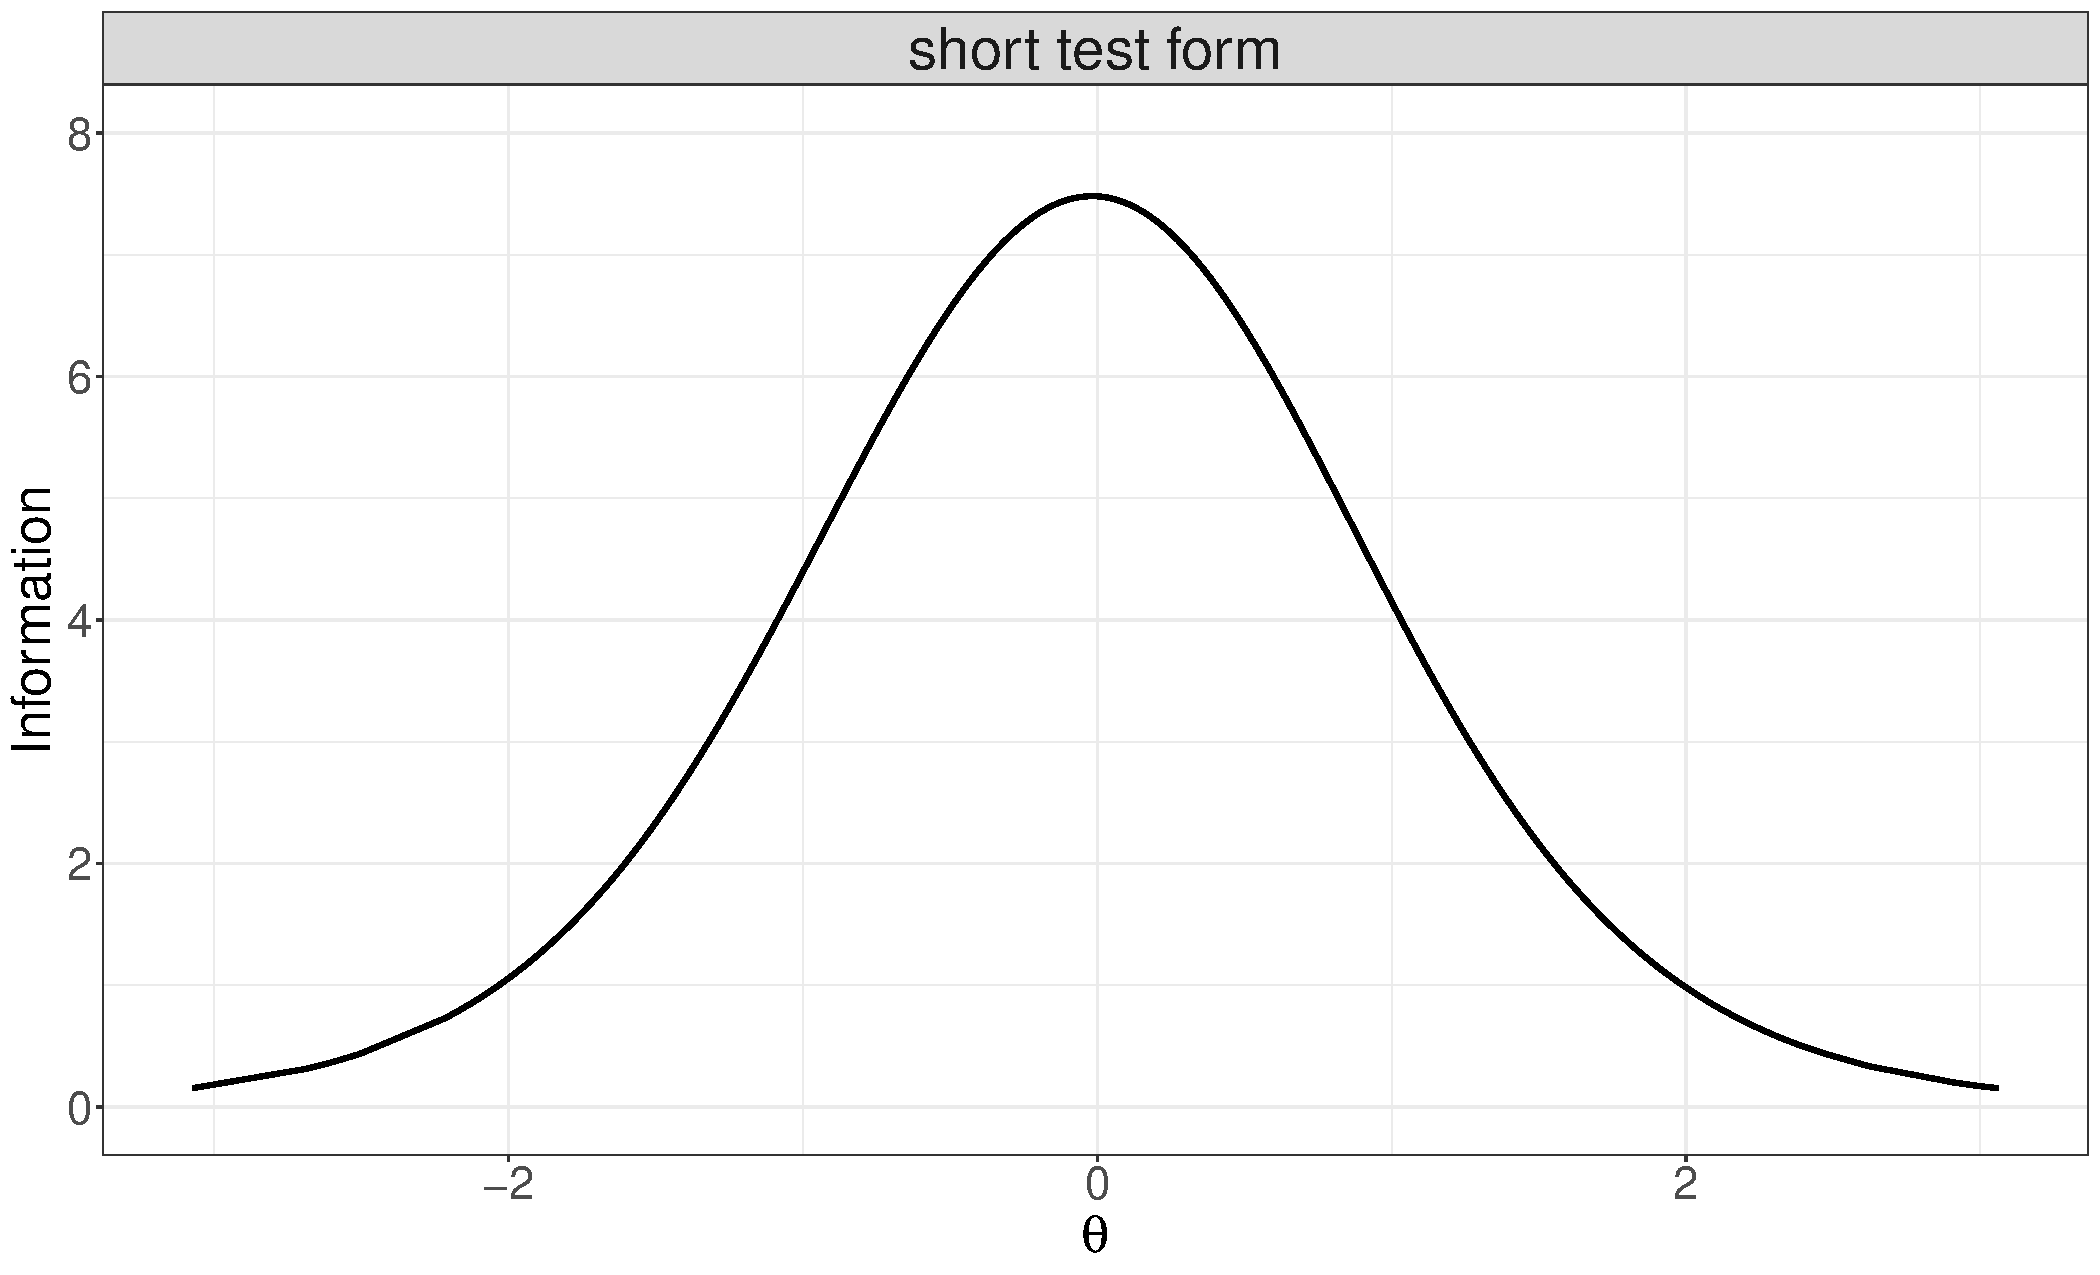
\includegraphics[width=.90\linewidth]{img/stf-bp}
	
	\onslide<2>
	\centering
	
	\texttt{plot\_tif(stf\_eip)}
	
	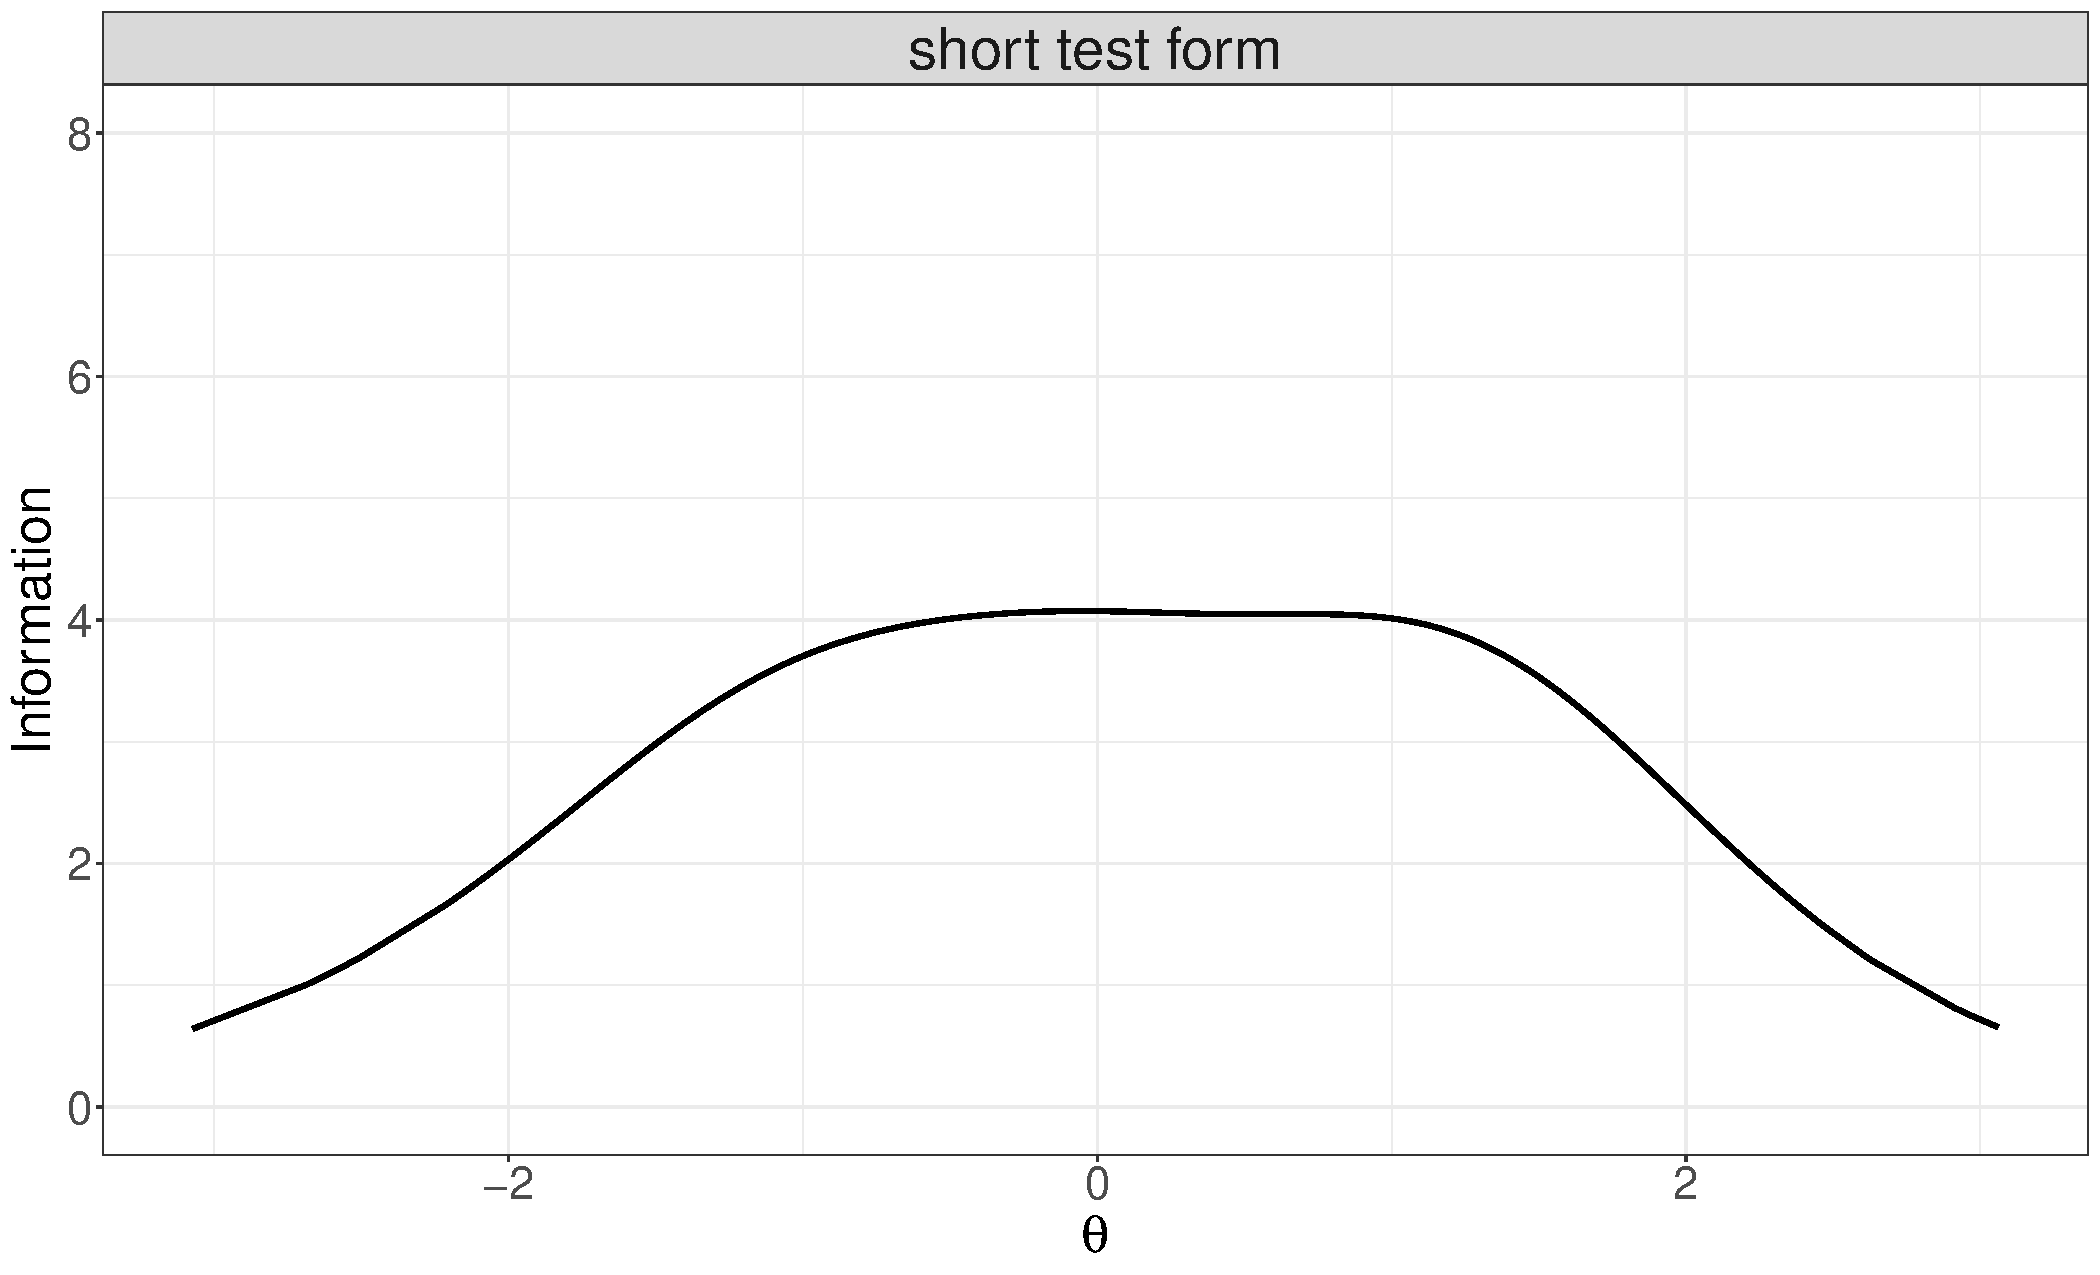
\includegraphics[width=.90\linewidth]{img/stf-eip}
	
	\onslide<3>
	\centering
	
	\texttt{plot\_tif(stf\_uip)}
	
	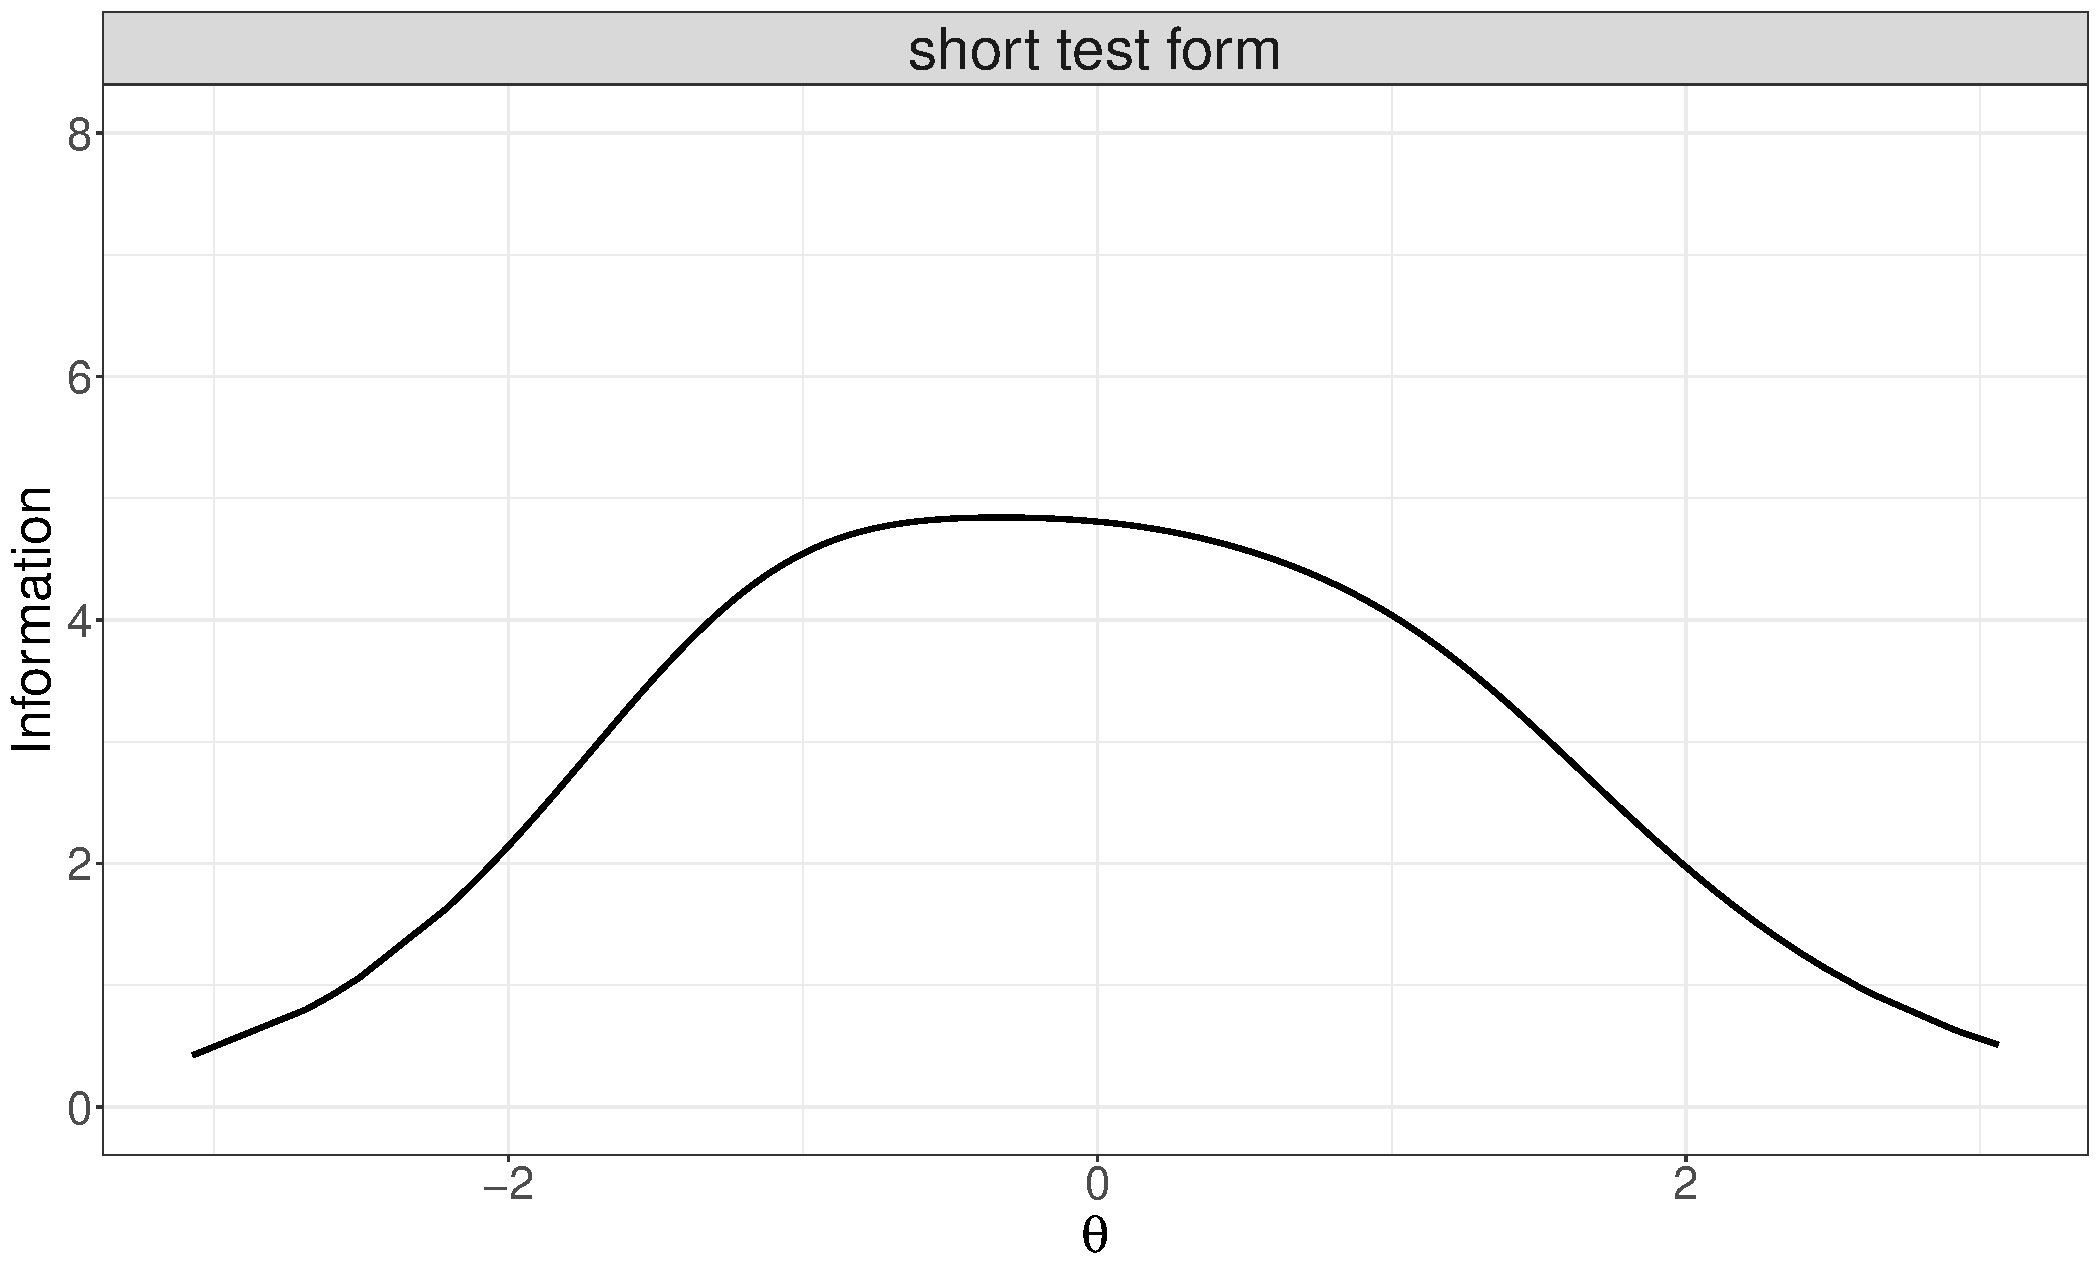
\includegraphics[width=.90\linewidth]{img/stf-uip}

\onslide<4>
\centering

All infos:

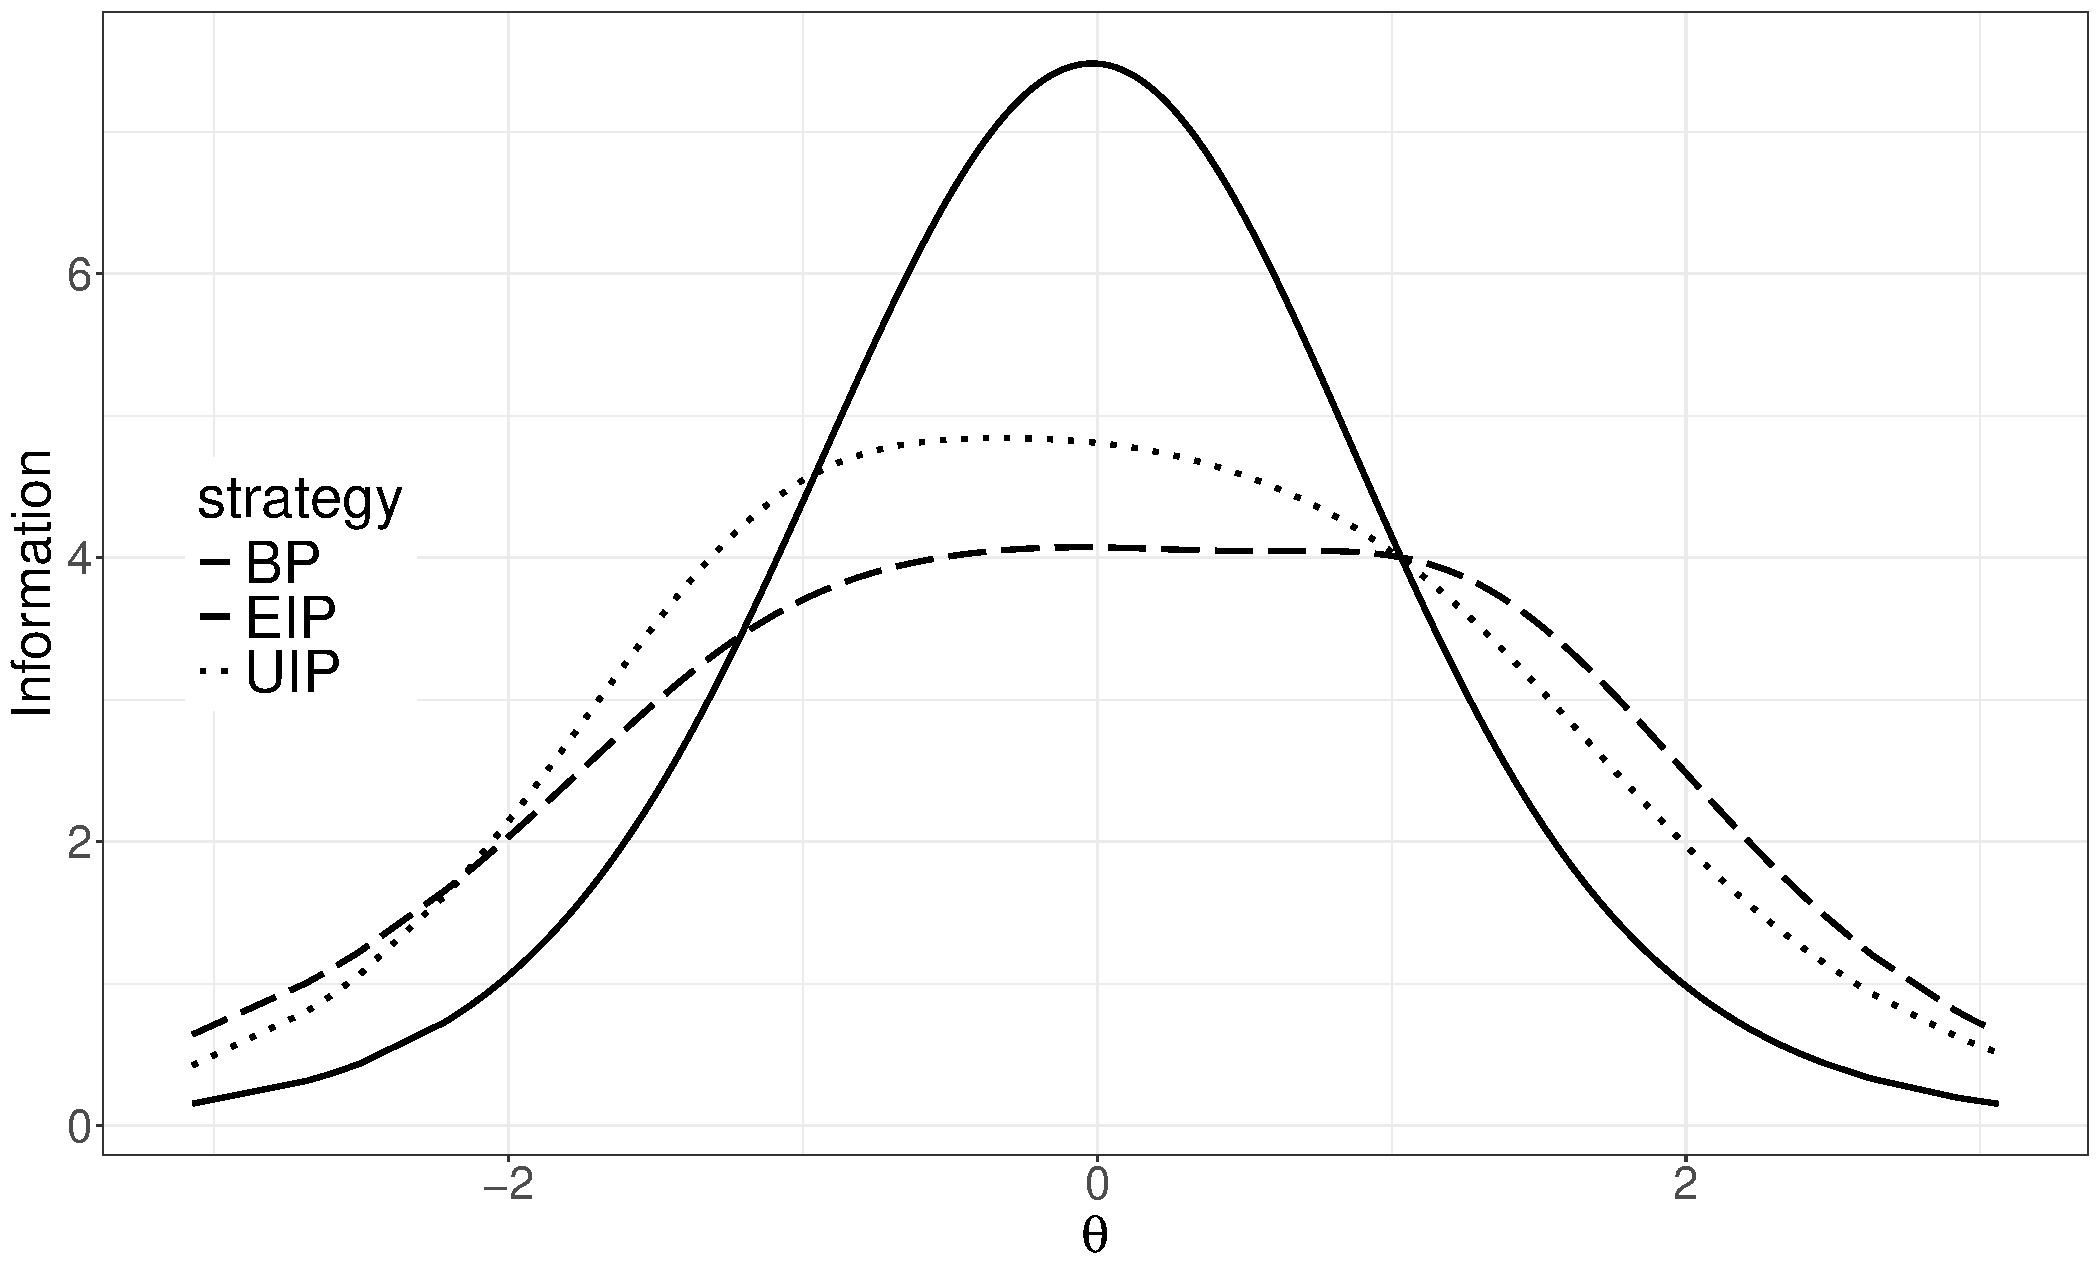
\includegraphics[width=.90\linewidth]{img/all-infos}

\end{overprint}
		

\end{frame}

\begin{frame}[fragile]

\begin{verbatim}
eip_difference  = diff_theta(stf_eip, starting_theta = true_theta)
\end{verbatim}

\begin{overprint}
\onslide<1>
\small
\begin{verbatim}
plot_difference(eip_difference, type = "diff", levels = 10) 
\end{verbatim}

\centering

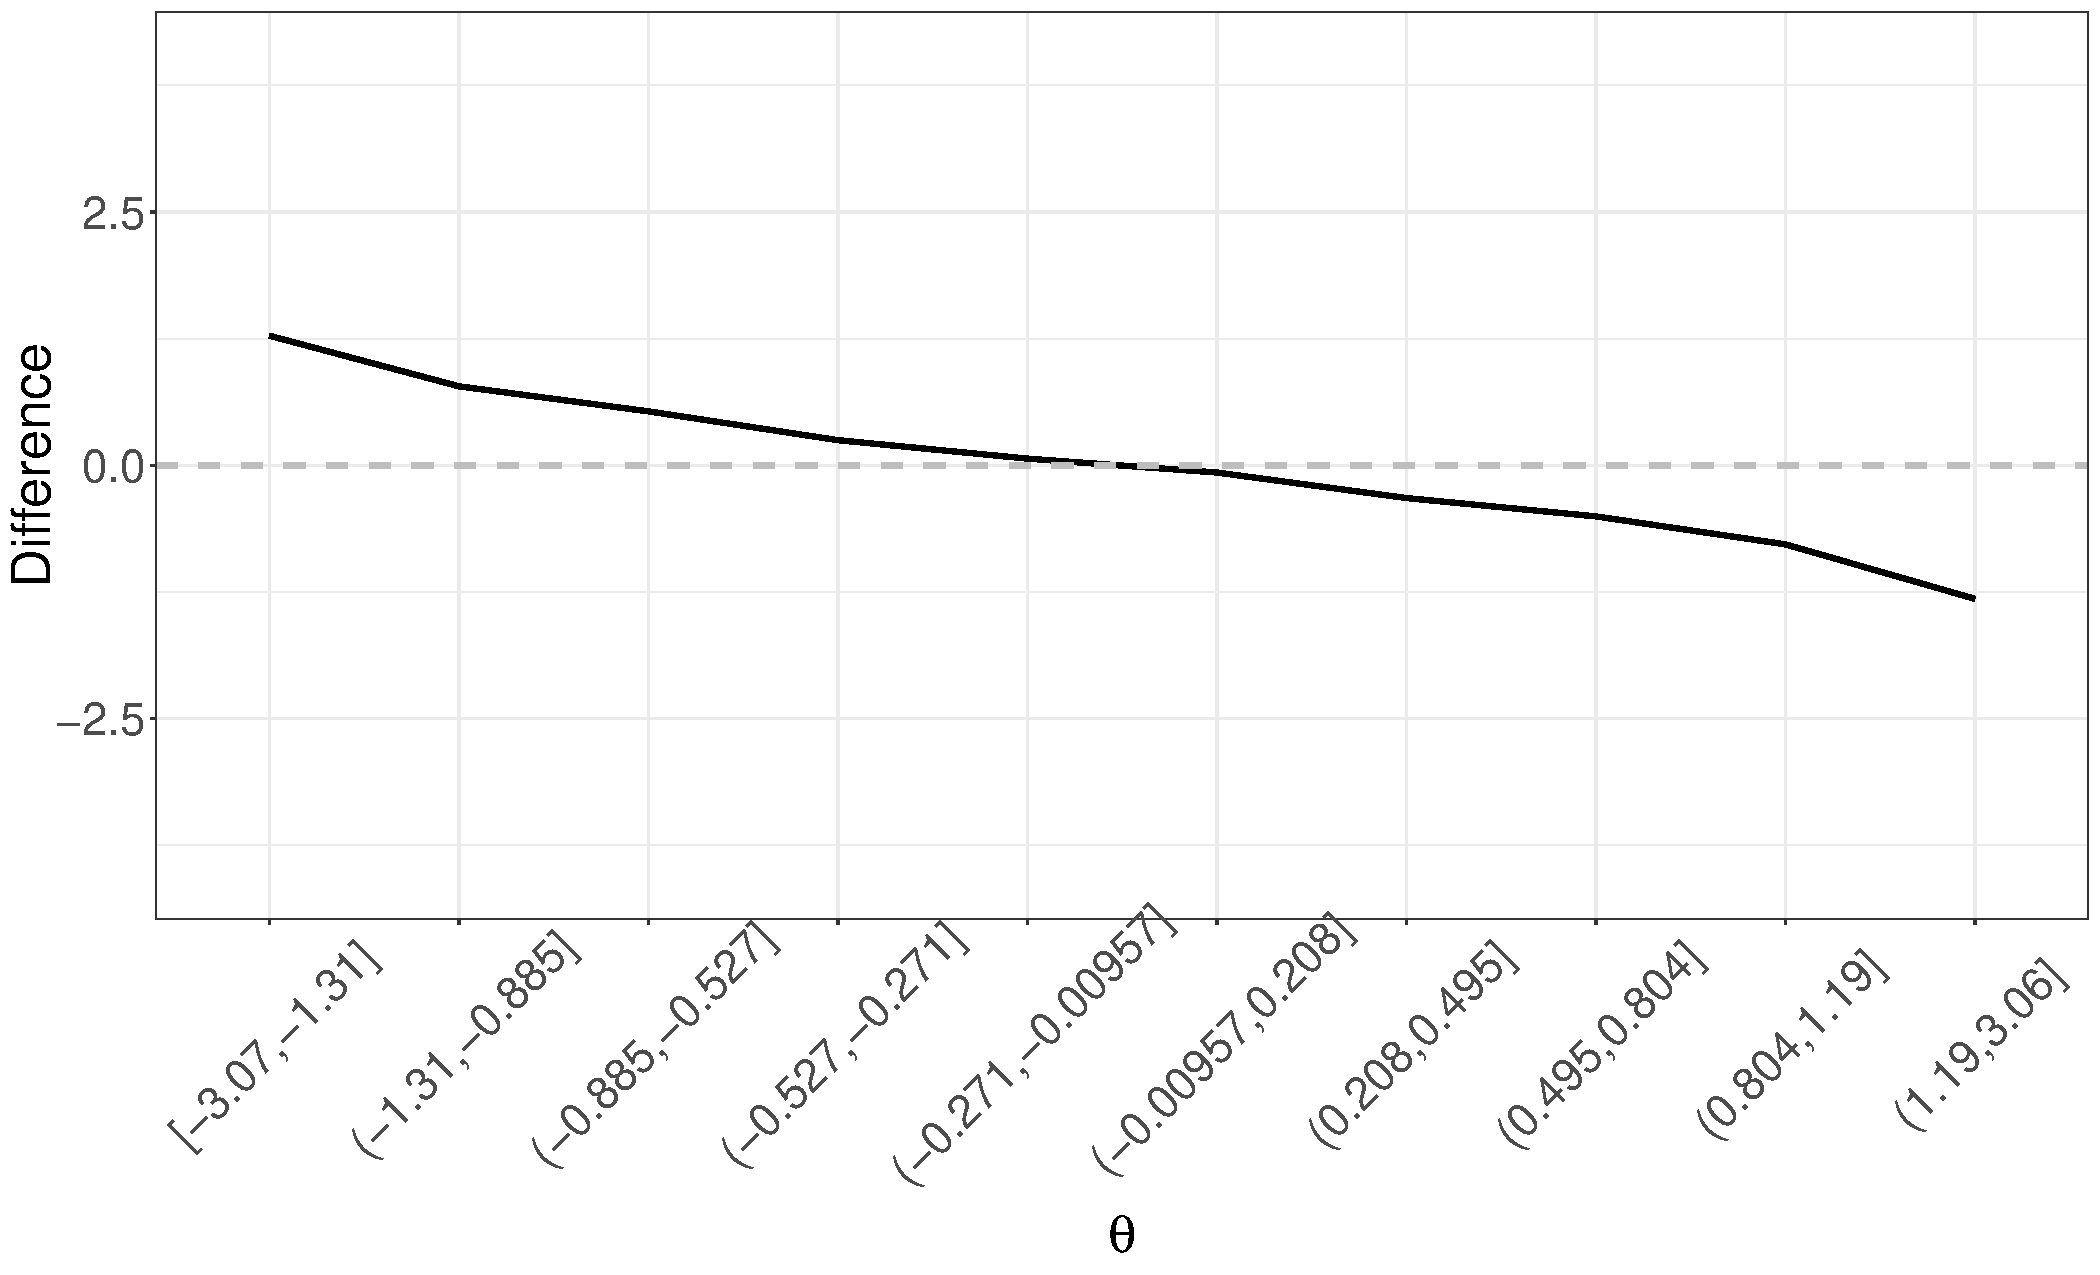
\includegraphics[width=.8\linewidth]{img/difference}


\onslide<2>
\small
\begin{verbatim}
plot_difference(eip_difference, type = "absolute_diff", levels = 10) 
\end{verbatim}

\centering

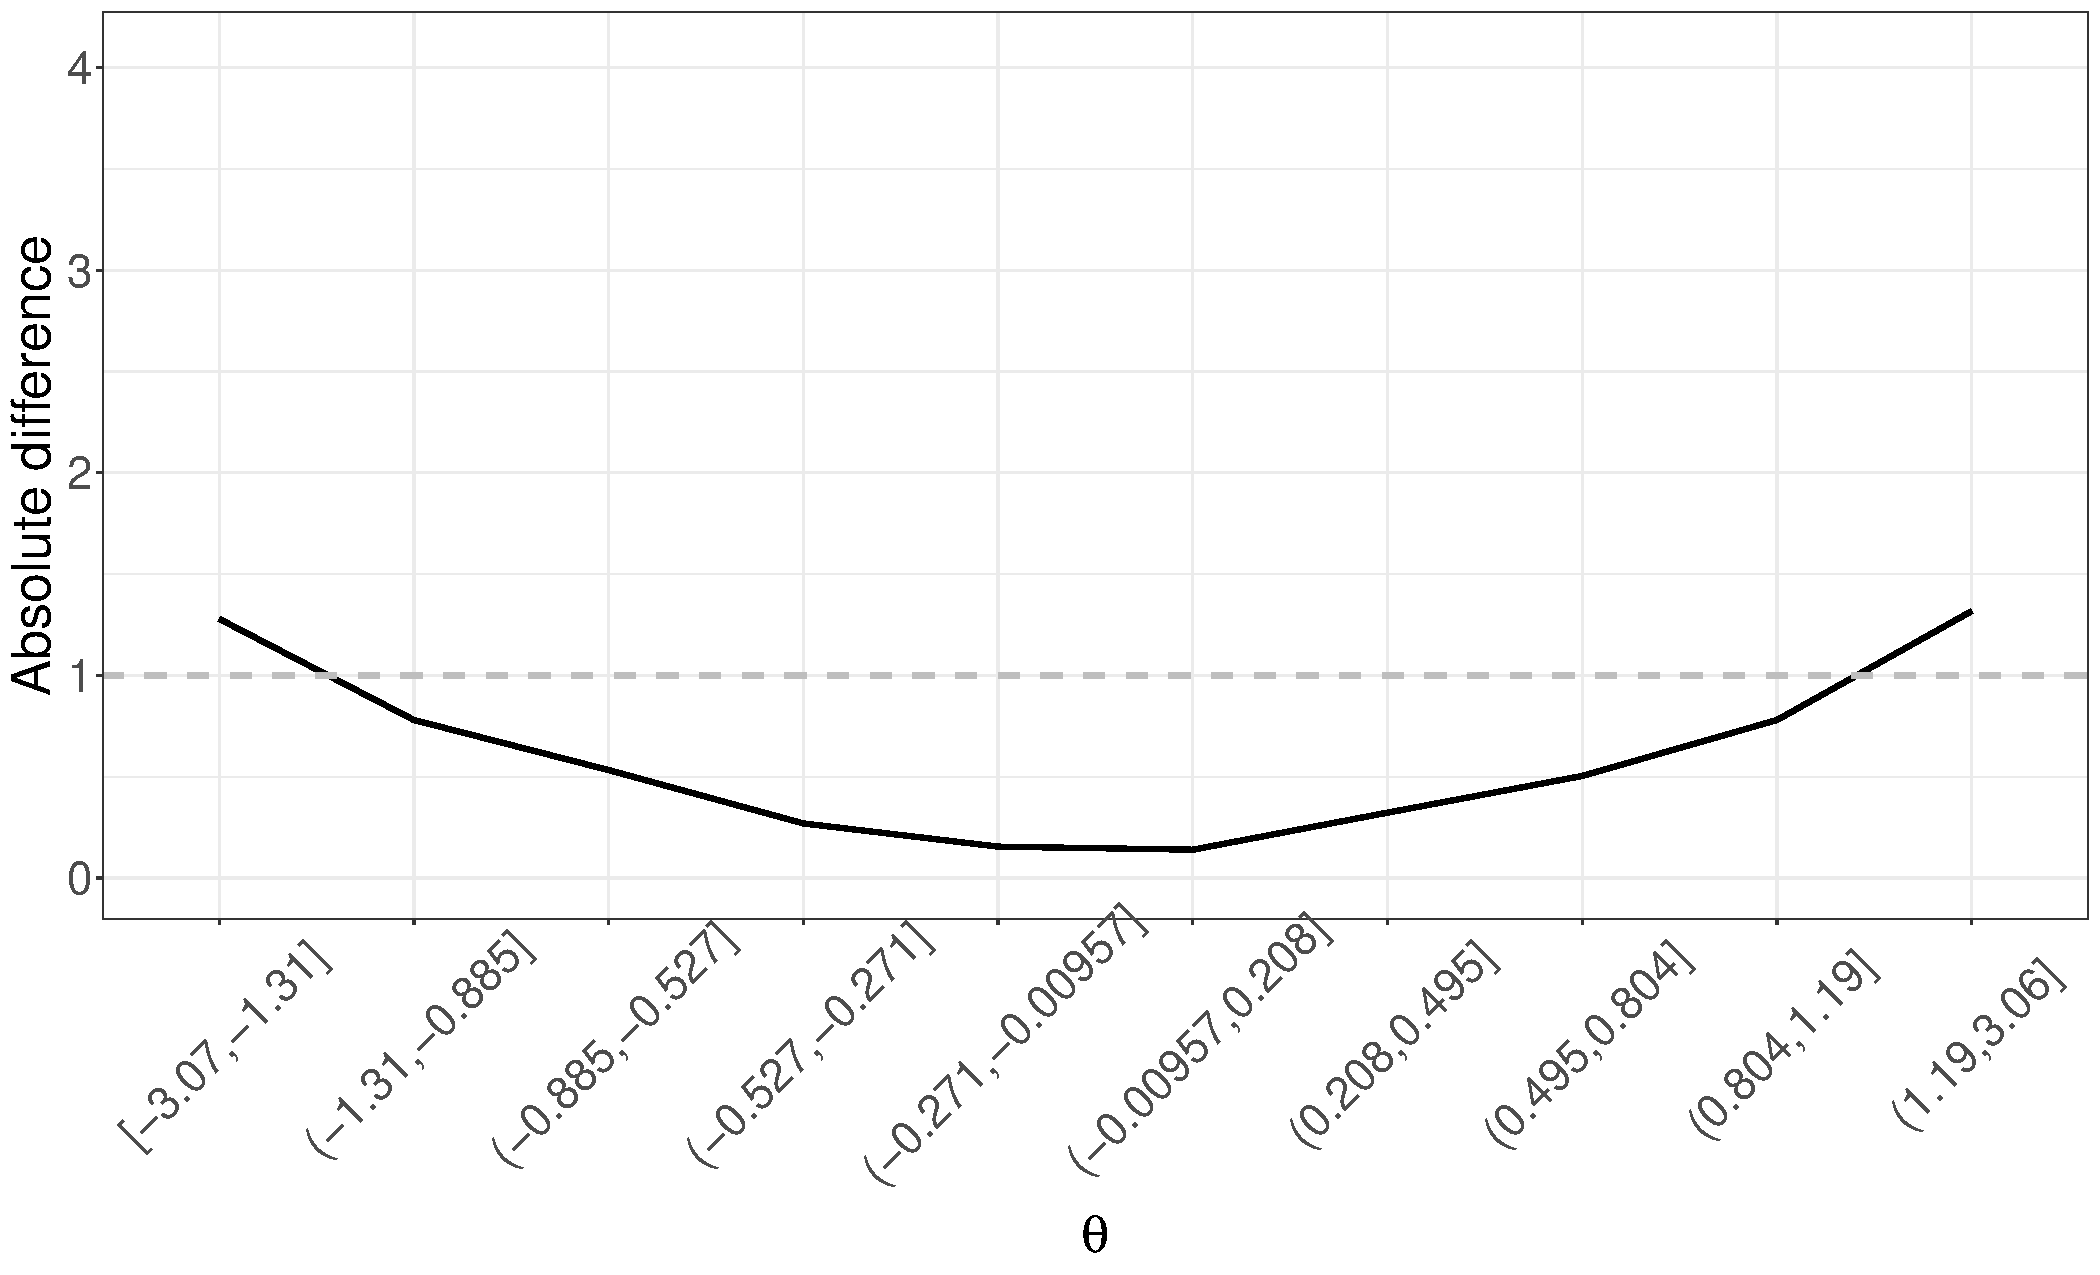
\includegraphics[width=.8\linewidth]{img/absolute-difference}
\end{overprint}


\end{frame}


\section[ILA]{Item Locating Algorithm}

\begin{frame}
	
	\begin{columns}[T]
		\begin{column}{.45\linewidth}
			
			\begin{center}
				\textbf{Set up:}
			\end{center}
			
			
			
			\vspace{1.5mm}
			\small
			$B$: Set of items of the item bank, items $i = \{1,2, \ldots, ||B||\}$
			
			\vspace{1.5mm}
			$Q^k \subset B$: Set of item selected for inclusion in the STF up to iteration $k$ ($Q^0 = \emptyset$)
			
			\vspace{1.5mm}
			$\mathbf{TIF}^*$: TIF target 
			
			\vspace{1.5mm}
			%$TIF^k = \frac{\sum_{i\in Q^k} IIF_i}{||Q^k||}$, where $||Q^k||$ denotes the cardinality of $Q^k$, 
			$\mathbf{TIF}^0 = (0, 0, \ldots, 0)$ 
			
		\end{column}
		
		\pause
		\begin{column}{.55\linewidth}
			\small 
			\centering
			\textbf{ILA Algorithm:} 
			\scalebox{.5}{
				\begin{tikzpicture}[node distance=2cm]
					
					% Nodes
					\node (start) [startstop] {Start, for $k \geq 1$};
					\node (target) [process, below of=start] {$\theta_{target} = \arg\max |\mathbf{TIF}^* - \mathbf{TIF}^{k-1}|$};
					\node (additem) [process, below of=target] {$Q^{k} = Q^{k-1} \cup \arg\min |\theta_{target} - b_i|$};
					\node (update) [process, below of=additem] {$\mathbf{TIF}^{k} = \frac{\sum_{i \in Q^k} \mathbf{IIF}_i}{||Q^k||}$};
					\node (check) [decision, right of=update, xshift=4cm] {$|\mathbf{TIF}^* - \mathbf{TIF}^k| \geq |\mathbf{TIF}^* - \mathbf{TIF}^{k-1}|$?};
					\node (stop) [startstop, below of=check, yshift=-3.5cm] {Stop \& Return $Q_{ILA} = Q^{k-1}$};
					
					% Arrows
					\draw [arrow] (start) -- (target);
					\draw [arrow] (target) -- (additem);
					\draw [arrow] (additem) -- (update);
					\draw [arrow] (update) -- (check);
					\draw [arrow] (check) -- node[anchor=east] {Yes} (stop);
					\draw [arrow] (check.east) -- ++(1,0) -- ++(0,4) -- node[anchor=north] {No, $k = k +1$} (target.east);
					
				\end{tikzpicture}
			}
			
		\end{column}
	\end{columns}
	
	
	
\end{frame}

\begin{frame}


		\begin{overprint}
	\onslide<1>
	\footnotesize
	

	
%	$\mathbf{TIF^*}$: TIF target describing the desired characteristic of a test
%	
%	$Q_{\text{ILA}}^k\subset B$: Set of items selected by ILA up to iteration $k$
	
	\centering
	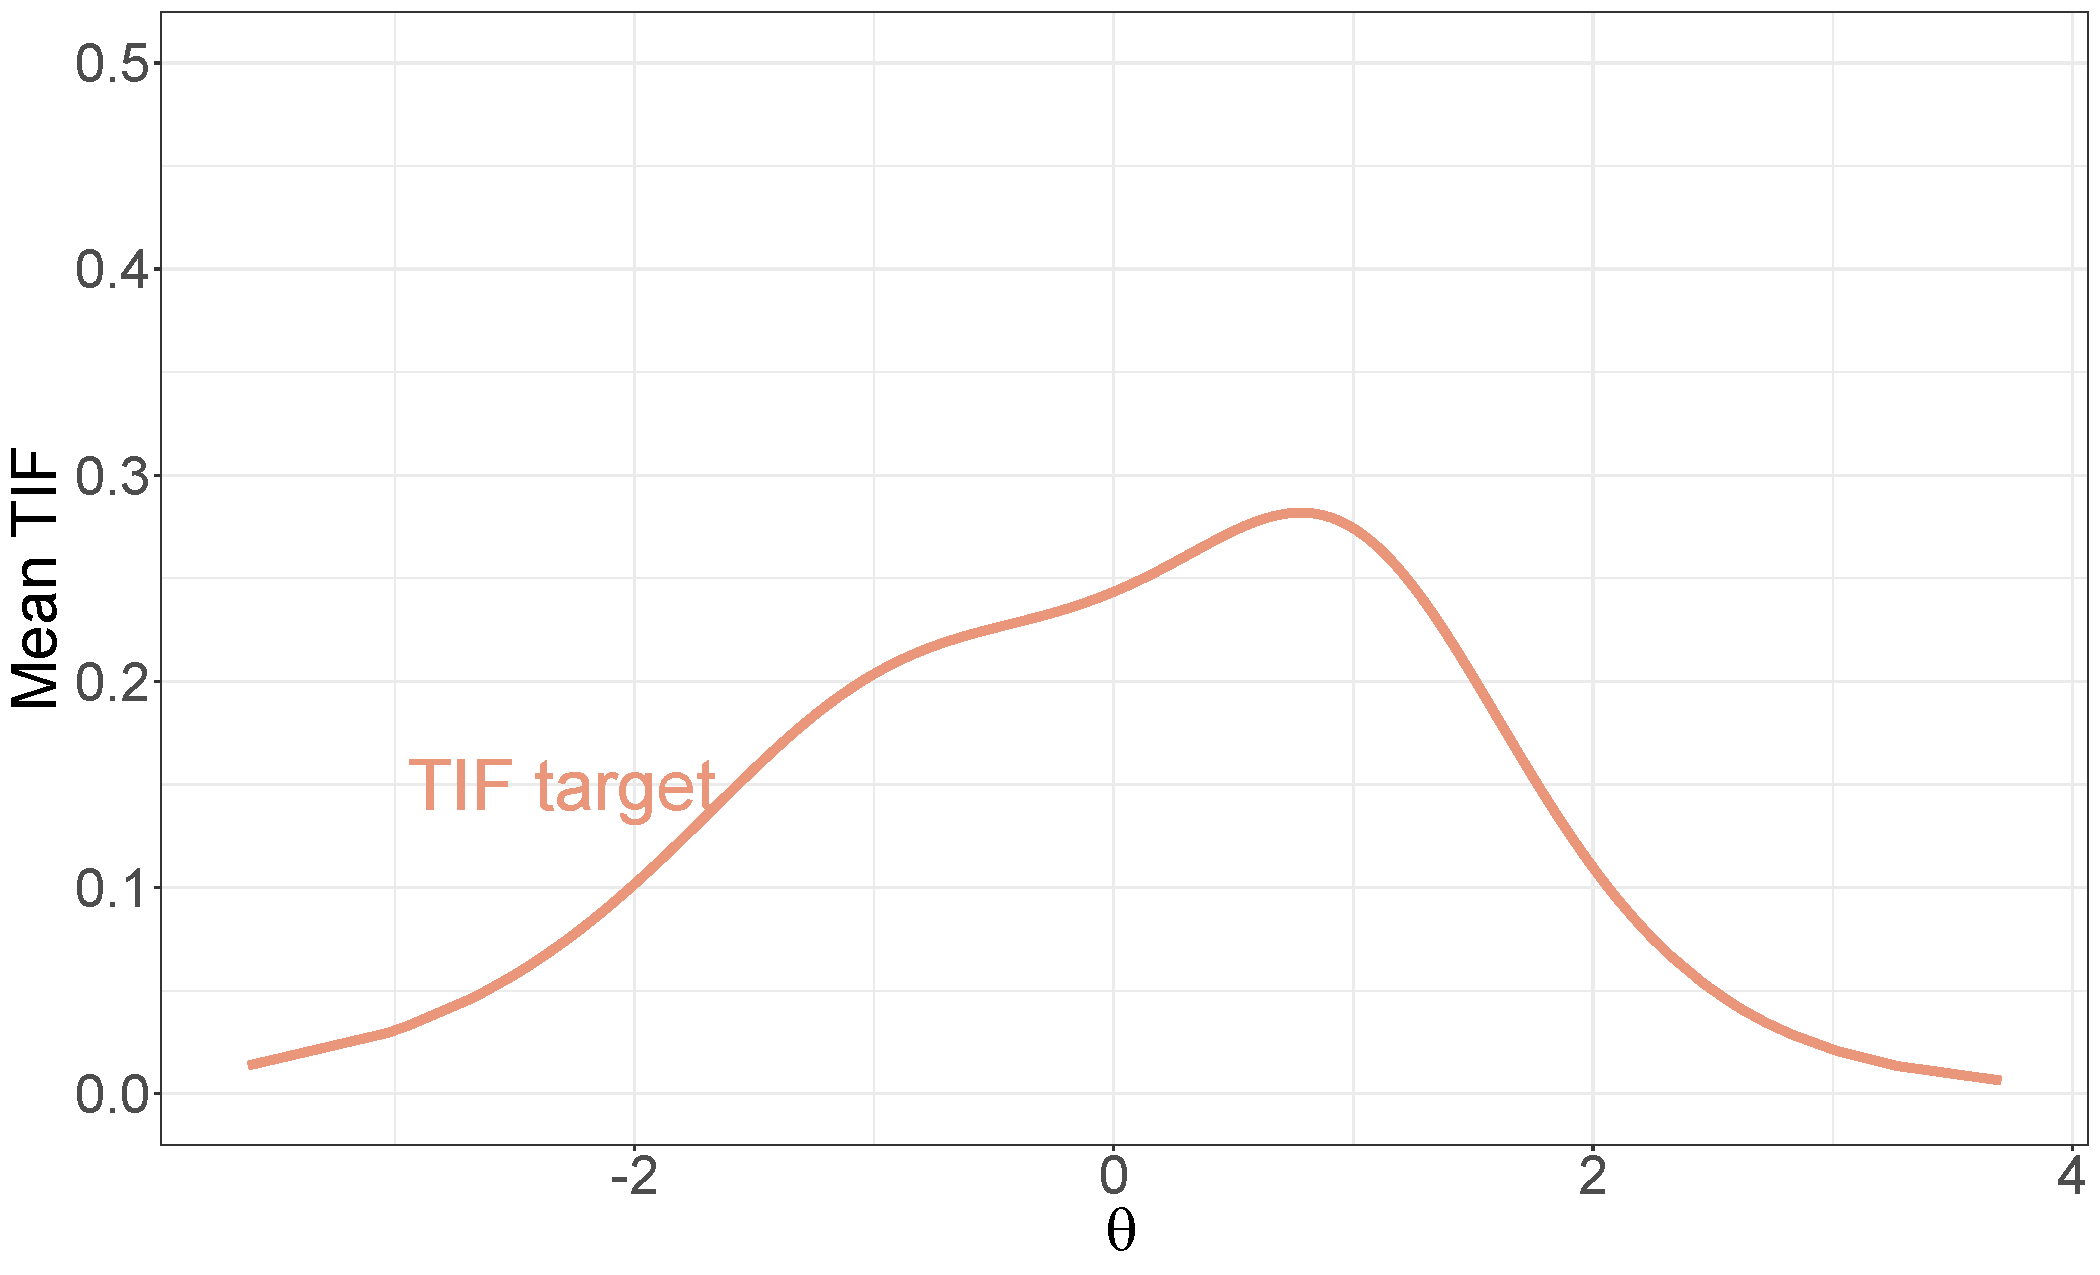
\includegraphics[width=.60\textwidth]{img/TIF-target.pdf}
	
	$k = 0$,	$Q^0 = \emptyset$, \\ $\theta_{target} := \arg\max |\mathbf{TIF}^* - \mathbf{TIF}^{0}|$, where $\mathbf{TIF^0} = (0, 0, \ldots, 0)$ \\
	
	
	\onslide<2>
	\centering
	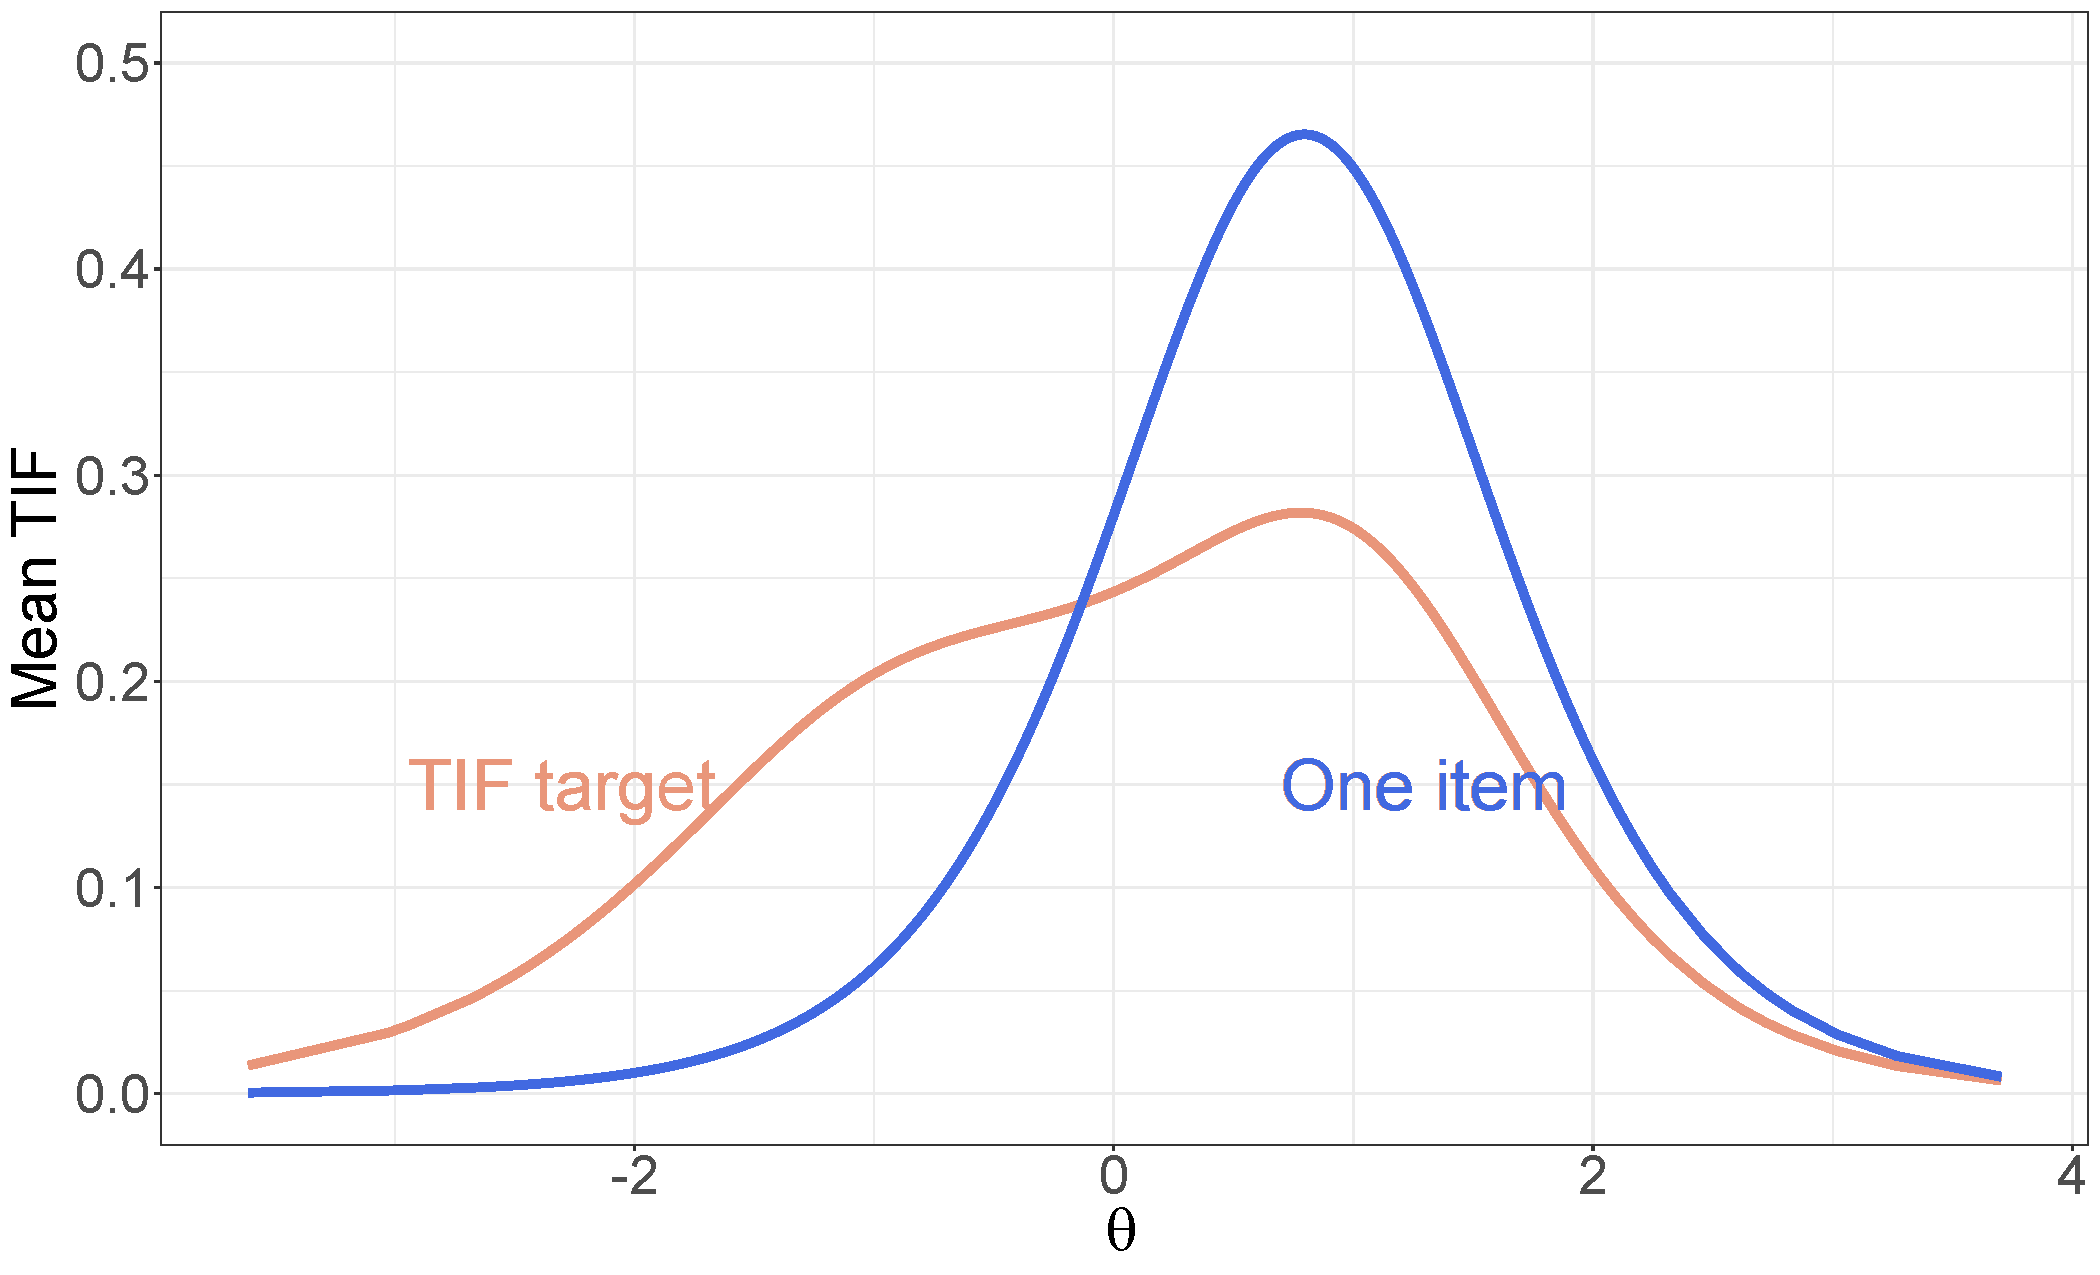
\includegraphics[width=.60\textwidth]{img/TIF-first.pdf}
	
	$k = 1$, $Q^1 = Q^{0} \cup \arg\min_{i \in B\setminus Q^0} |\theta_{target} - b_i|$, 	$||Q^1|| = 1$ 
	$|\mathbf{TIF}^* - \mathbf{TIF}^1| \geq |\mathbf{TIF}^* - \mathbf{TIF}^{0}|$ $\rightarrow$ \texttt{false}, $k = 2$\\
	$\theta_{target} := \arg\max |\mathbf{TIF}^* - \mathbf{TIF}^{1}|$\\
	
	\onslide<3>\centering
	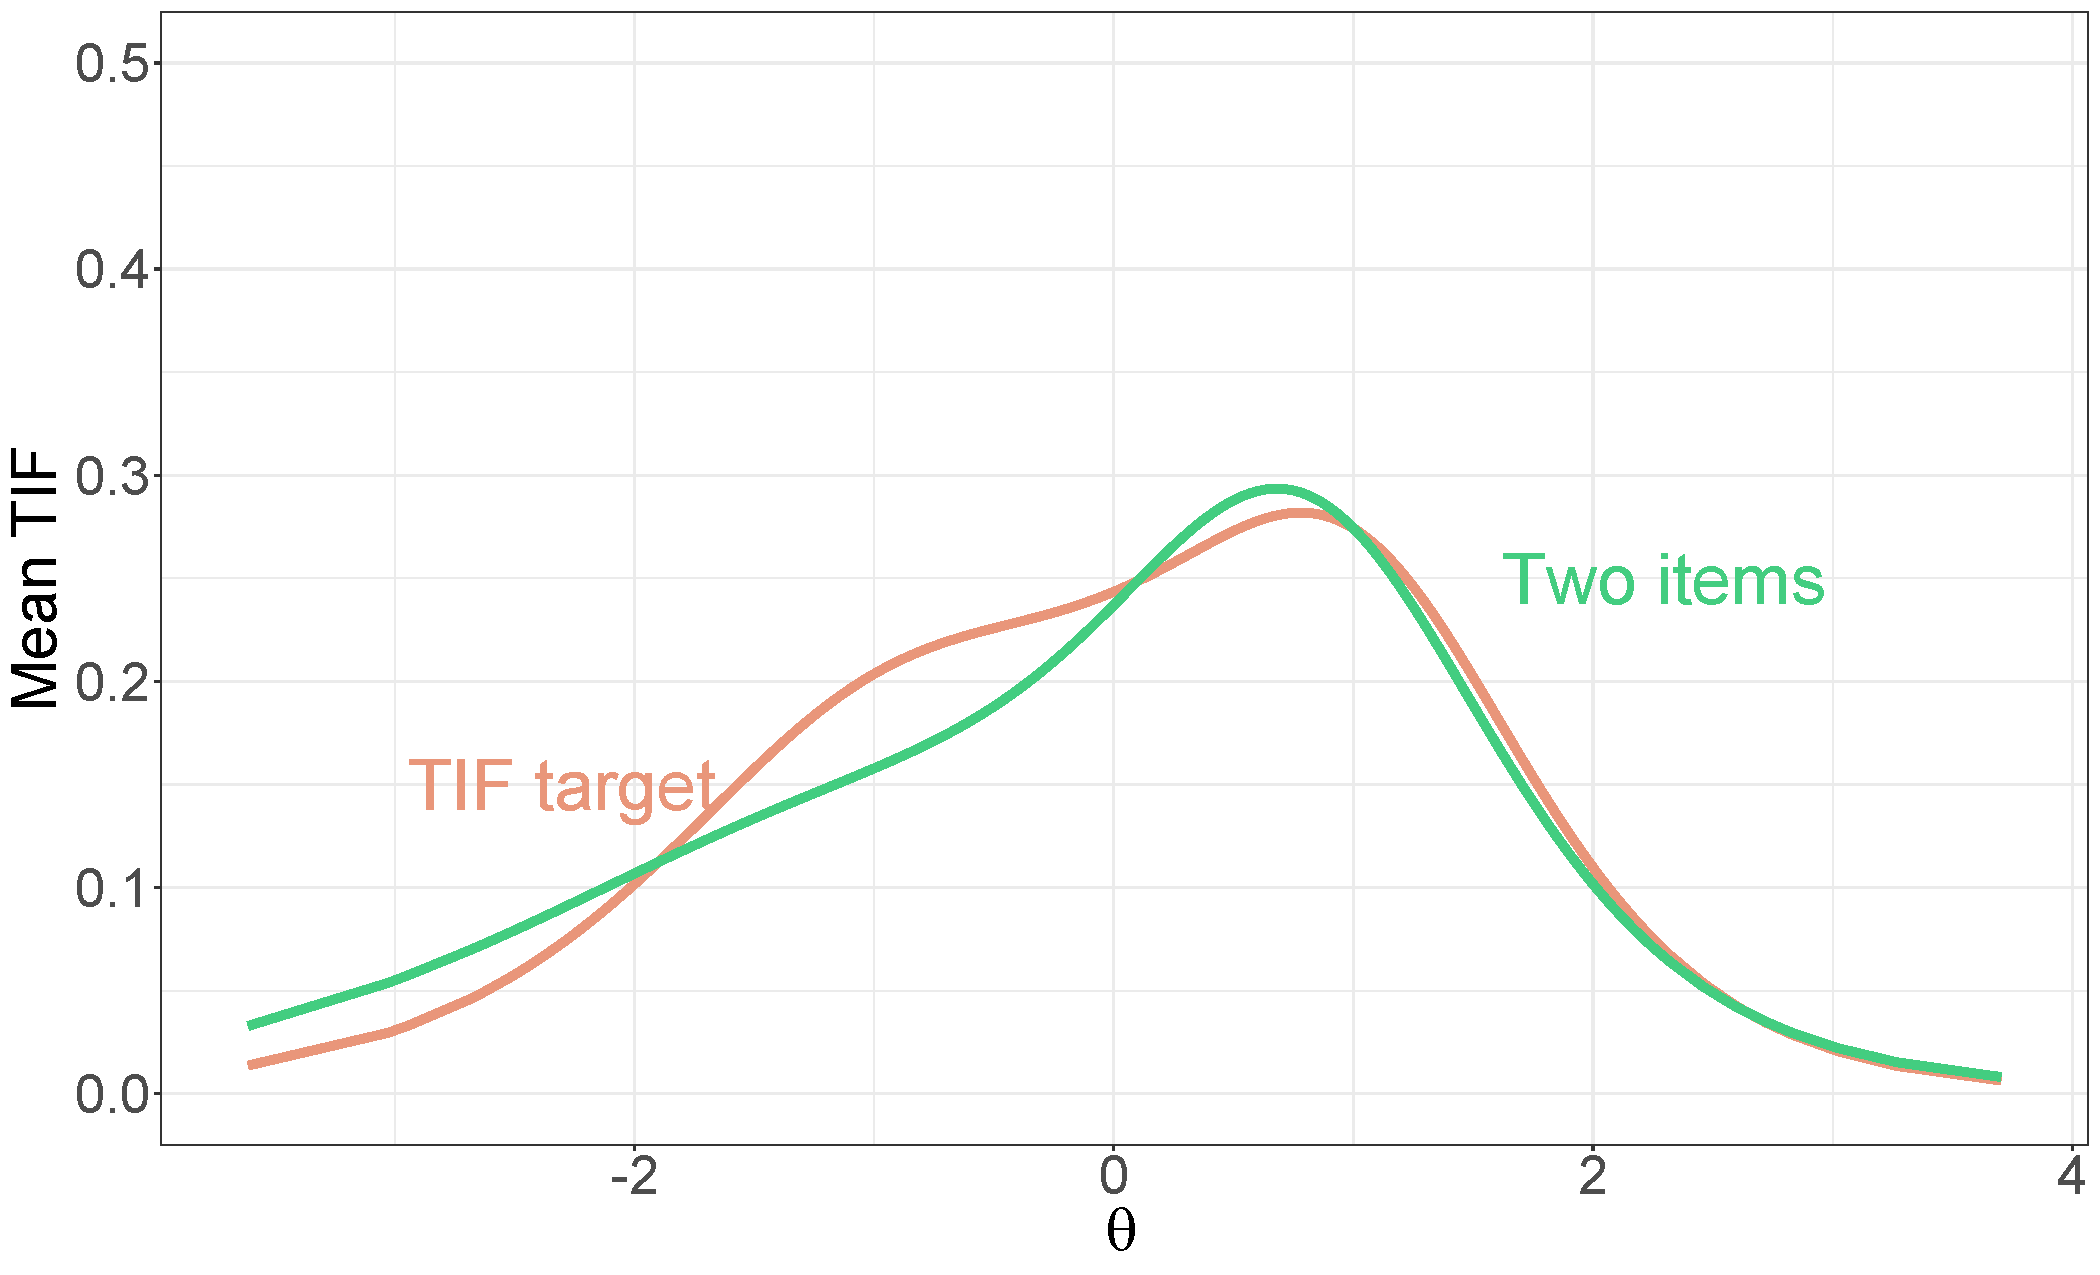
\includegraphics[width=.60\textwidth]{img/TIF-second.pdf}
	
	$Q^2 = Q^{1} \cup \arg\min_{i \in B\setminus Q^1} |\theta_{target} - b_i|$, 	$||Q^2|| = 2$
	$|\mathbf{TIF}^* - \mathbf{TIF}^2| \geq |\mathbf{TIF}^* - \mathbf{TIF}^{1}|$ $\rightarrow$ \texttt{false}, $k = 3$\\
	$\theta_{target} := \arg\max |\mathbf{TIF}^* - \mathbf{TIF}^{2}|$\\
	\onslide<4>
	\centering
	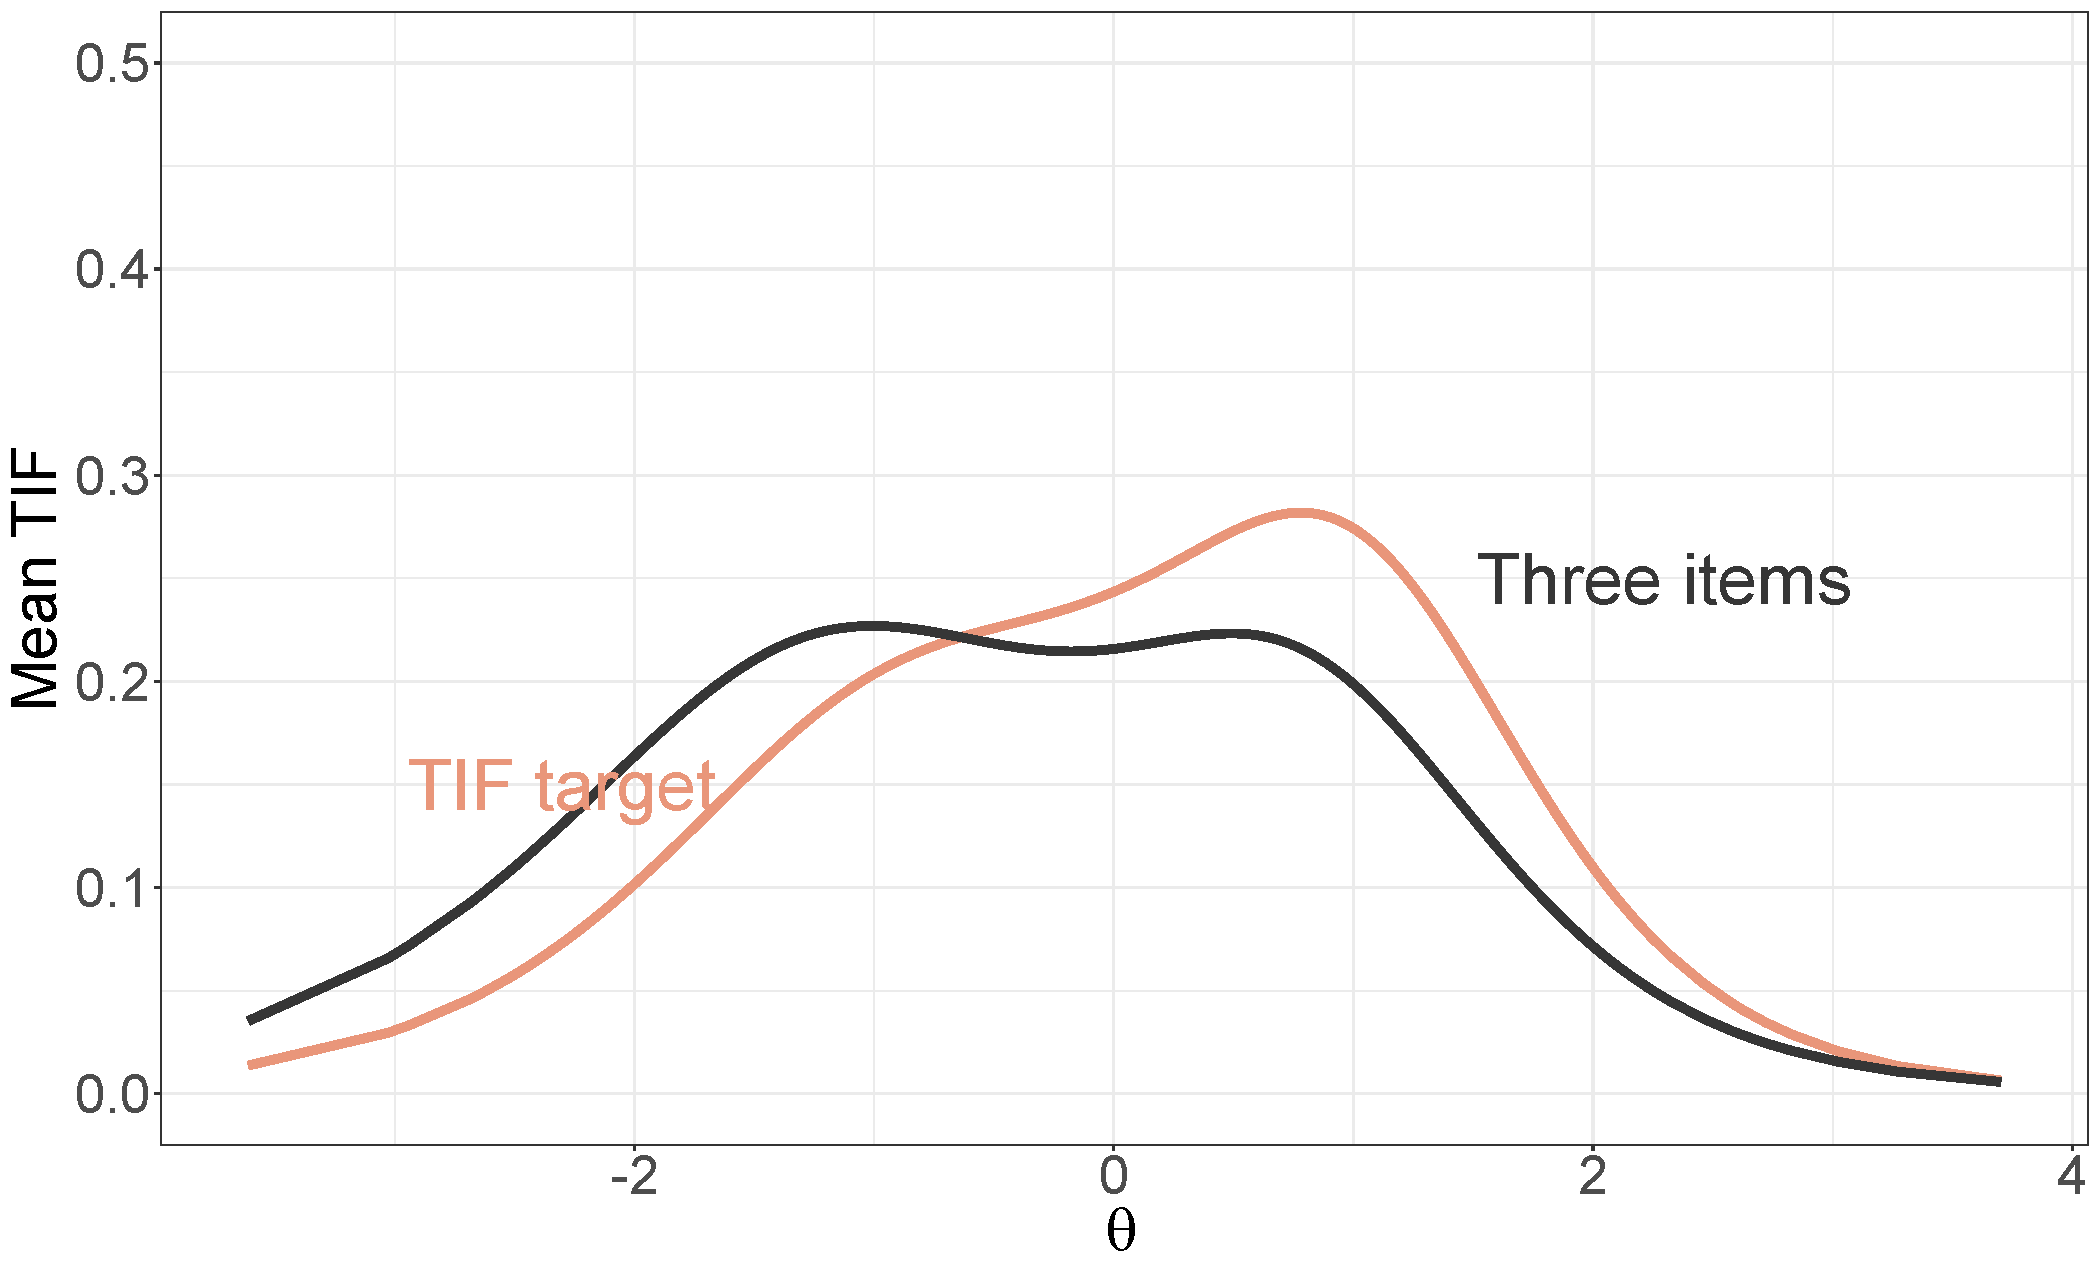
\includegraphics[width=.60\textwidth]{img/TIF-third.pdf}
	
	$Q^3 = Q^{2} \cup \arg\min_{i \in B\setminus Q^2} |\theta_{target} - b_i|$, 	$||Q^3|| = 3$ \\
	$|\mathbf{TIF}^* - \mathbf{TIF}^3| \geq |\mathbf{TIF}^* - \mathbf{TIF}^{2}|$ $\rightarrow$ \texttt{true} $\rightarrow$ \textbf{end}, $Q_{\textbf{ILA}} = Q^2$
\end{overprint}
\end{frame}

\begin{frame}{Brute Force Procedure -- BFP}
	

	Item bank $B$\\
	$Q_m \subset B$ item combinations of different lengths $l = 1, 2, \ldots, ||B||-1$\\ Total number of item combinations $2^{||B||}-2$\\
	$\overline{\Delta}_{\mathbf{TIF}^{Q_m}} =  \mathit{mean}(|\mathbf{TIF}^* - \dfrac{\sum_{i \in Q_m} IIF_i}{||Q_m||}|)$ \\
	$Q_{BFP} = \arg \min_{\emptyset \neq Q_m \subset Q} \overline{\Delta}_{\mathbf{TIF}^{Q_m}}$
	

\end{frame}


\subsection*{Simulation design}
\begin{frame}
	
	\small
	\textbf{100 data frames}:
	
	\begin{enumerate}
		\item  Generate an item bank $||B|| = 6$ items: 
		\begin{itemize}
			\item Difficulty parameters: $\mathcal{U}(-3, 3)$
			\item Discrimination parameters:  $\mathcal{U}(.90, 2.0)$
		\end{itemize} 
		
		\item  Random item selections of lengths $l$ from $B$ ($M_l = 3.34 \pm 1.13$) + modification parameters $\mathcal{U}(-0.20, 0.20)$ $\rightarrow$ $\mathbf{TIF}^*$ 
		
		\item  Considering $\mathbf{TIF}^*$ at Step 2 and item parameters at Step 1:
		\begin{itemize}
			\item ILA  $\rightarrow$ \emph{Forwardly searches} %the item selection best able to recover the $TIF^*$
			\item BFP  $\rightarrow$ \emph{Systematically tests} % every item combination to find the one best able to recover $TIF^*$. \\ 
			%	\small $N=6$ $\rightarrow$ $62$ STFs
		\end{itemize}
		
	\end{enumerate}
	
	\textbf{Comparison}:
	
	\begin{itemize}
		\item $||Q_{\text{BFP}}|| - ||Q_{\text{ILA}}||$ 
		\item Percentile rank (RP) of the distance $\mathbf{TIF}_{\text{BFP}} - \mathbf{TIF}_{\text{ILA}}$   
	\end{itemize}
	
	
\end{frame}

\subsection*{$||Q_{BFP}||$ vs. $||Q_{ILA}||$}

\begin{frame}
	$||Q_{\text{BFP}}|| - ||Q_{\text{ILA}}|| = 0$ in 57\% of cases % $\rightarrow$ 72\% same item selection
	\begin{figure}
		\centering
		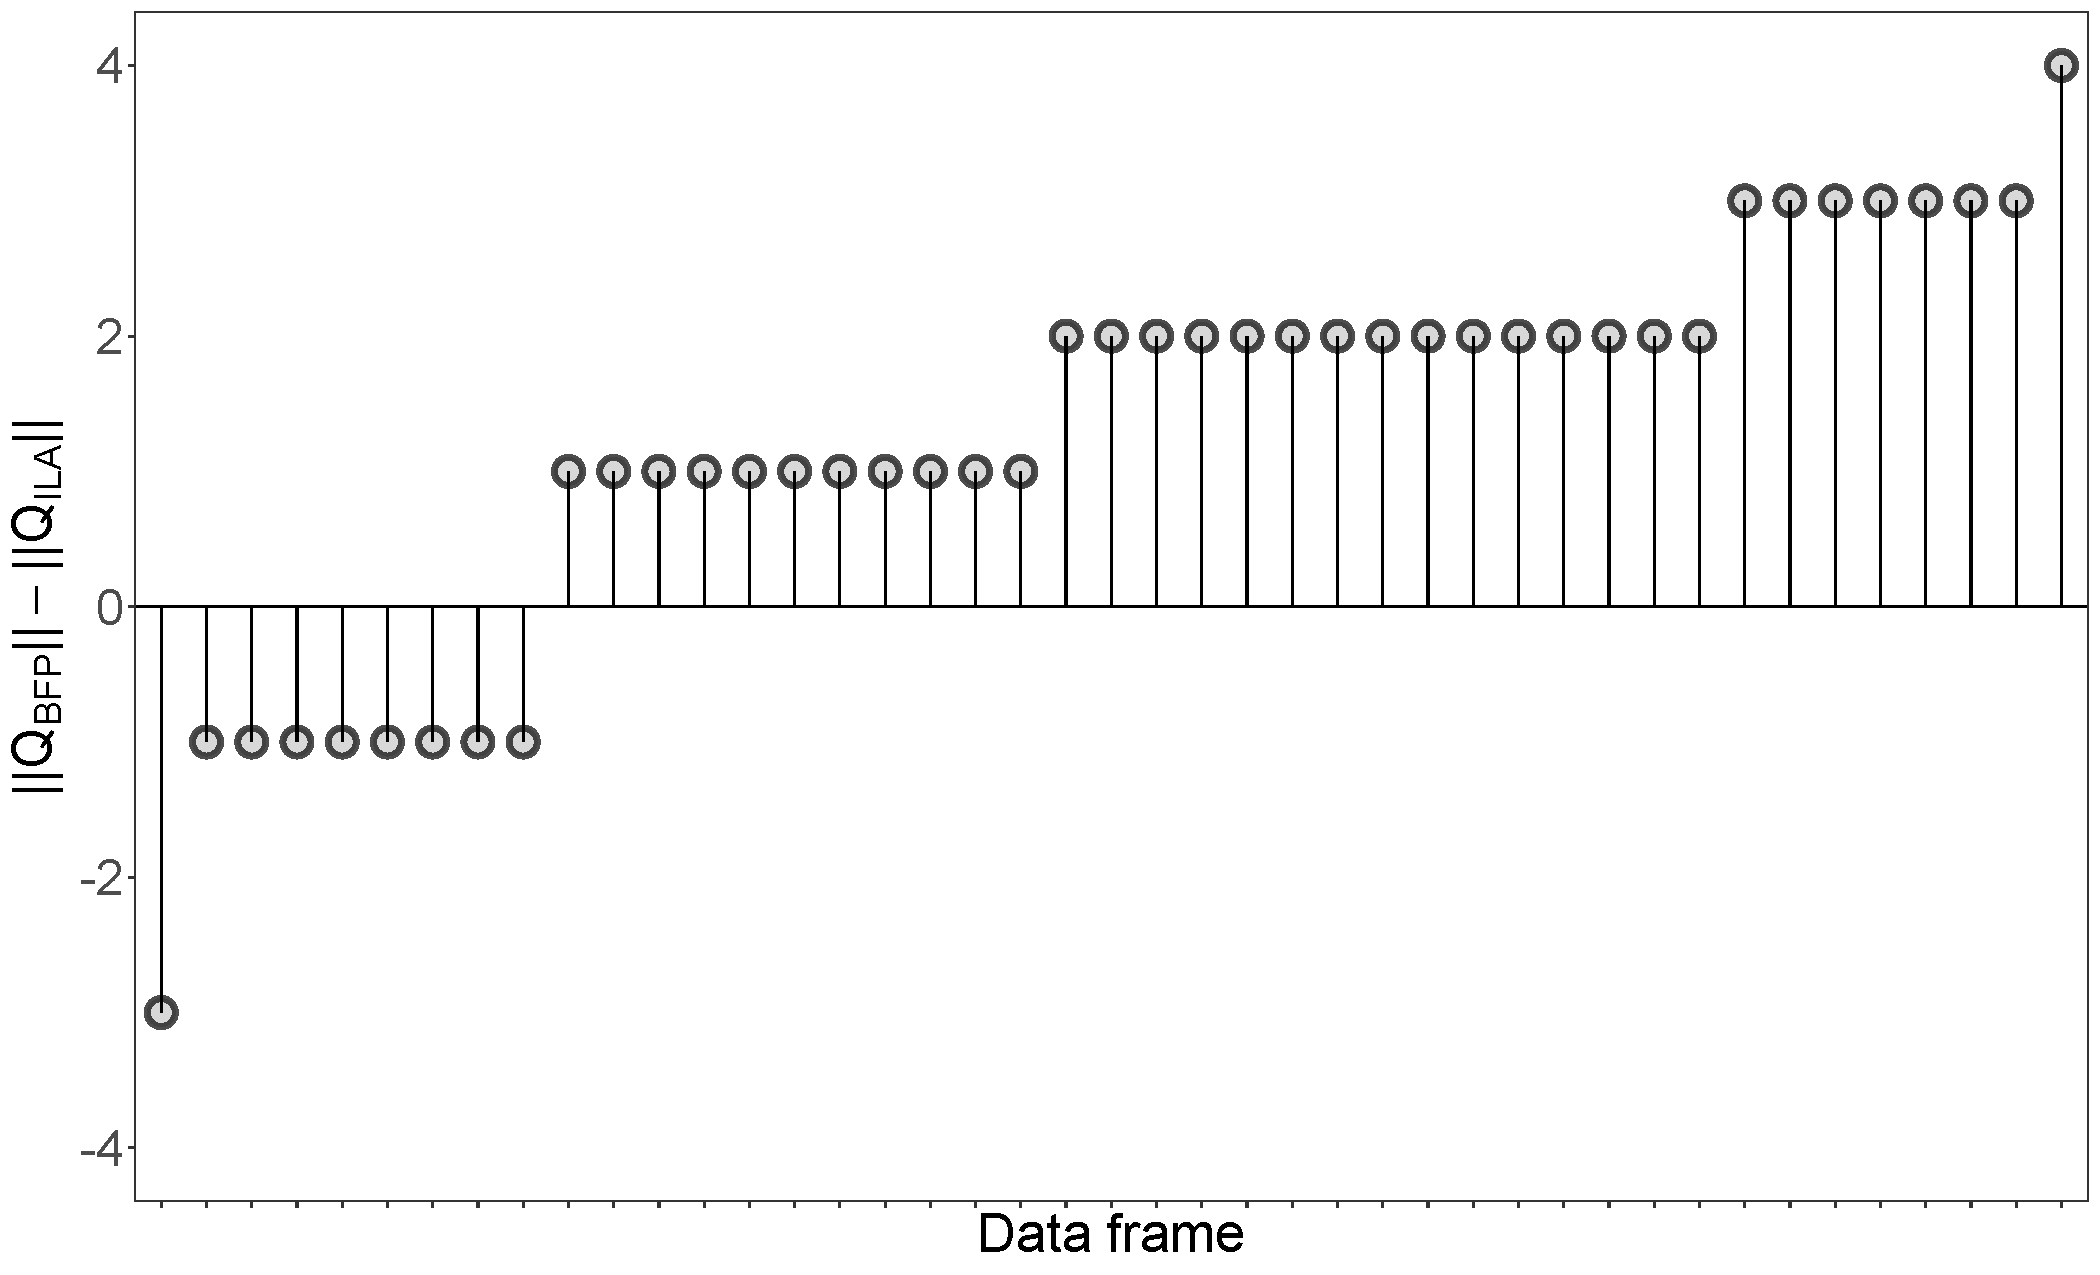
\includegraphics[width=.80\linewidth]{img/bfp-ila}
		%\caption{43\% $\rightarrow$ $||Q_{\text{BFP}}|| - ||Q_{\text{ILA}}|| \neq 0$ }
	\end{figure}
\end{frame}

\subsection*{Distance}

\begin{frame}
	\begin{figure}
		\centering
		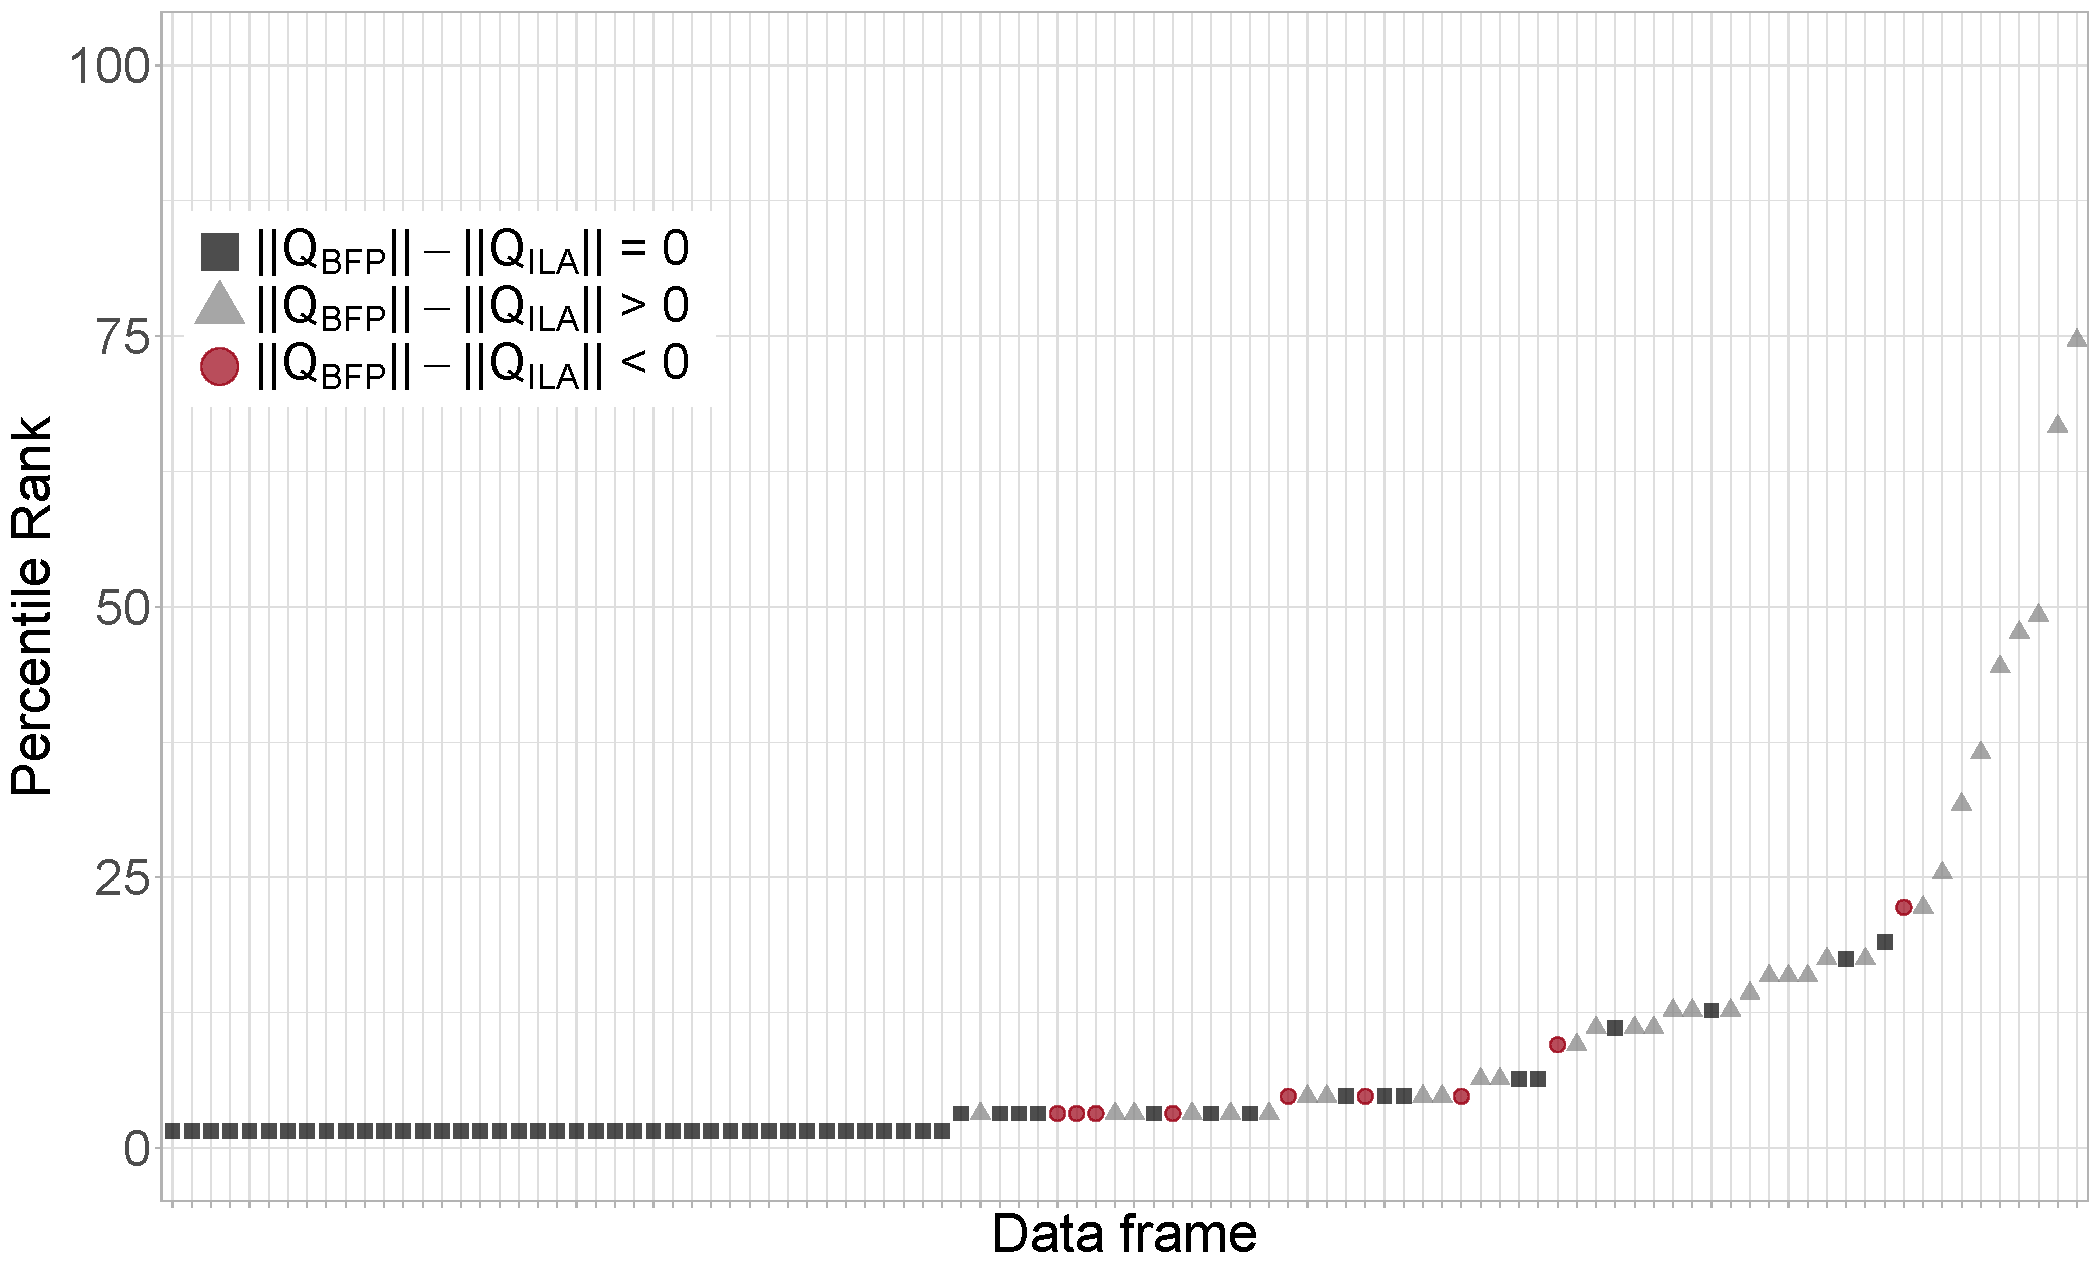
\includegraphics[width=.9\linewidth]{img/rp}
	\end{figure}
\end{frame}

\subsection*{TIF comparison}

\begin{frame}
	
	\begin{columns}[T]
		\begin{column}{.50\linewidth}
			
			\centering
			\footnotesize{$||Q_{\text{BFP}}|| = ||Q_{\text{ILA}}||$, $Q_{\text{BFP}} \neq Q_{\text{ILA}}$, $RP = 3.17$}
			
			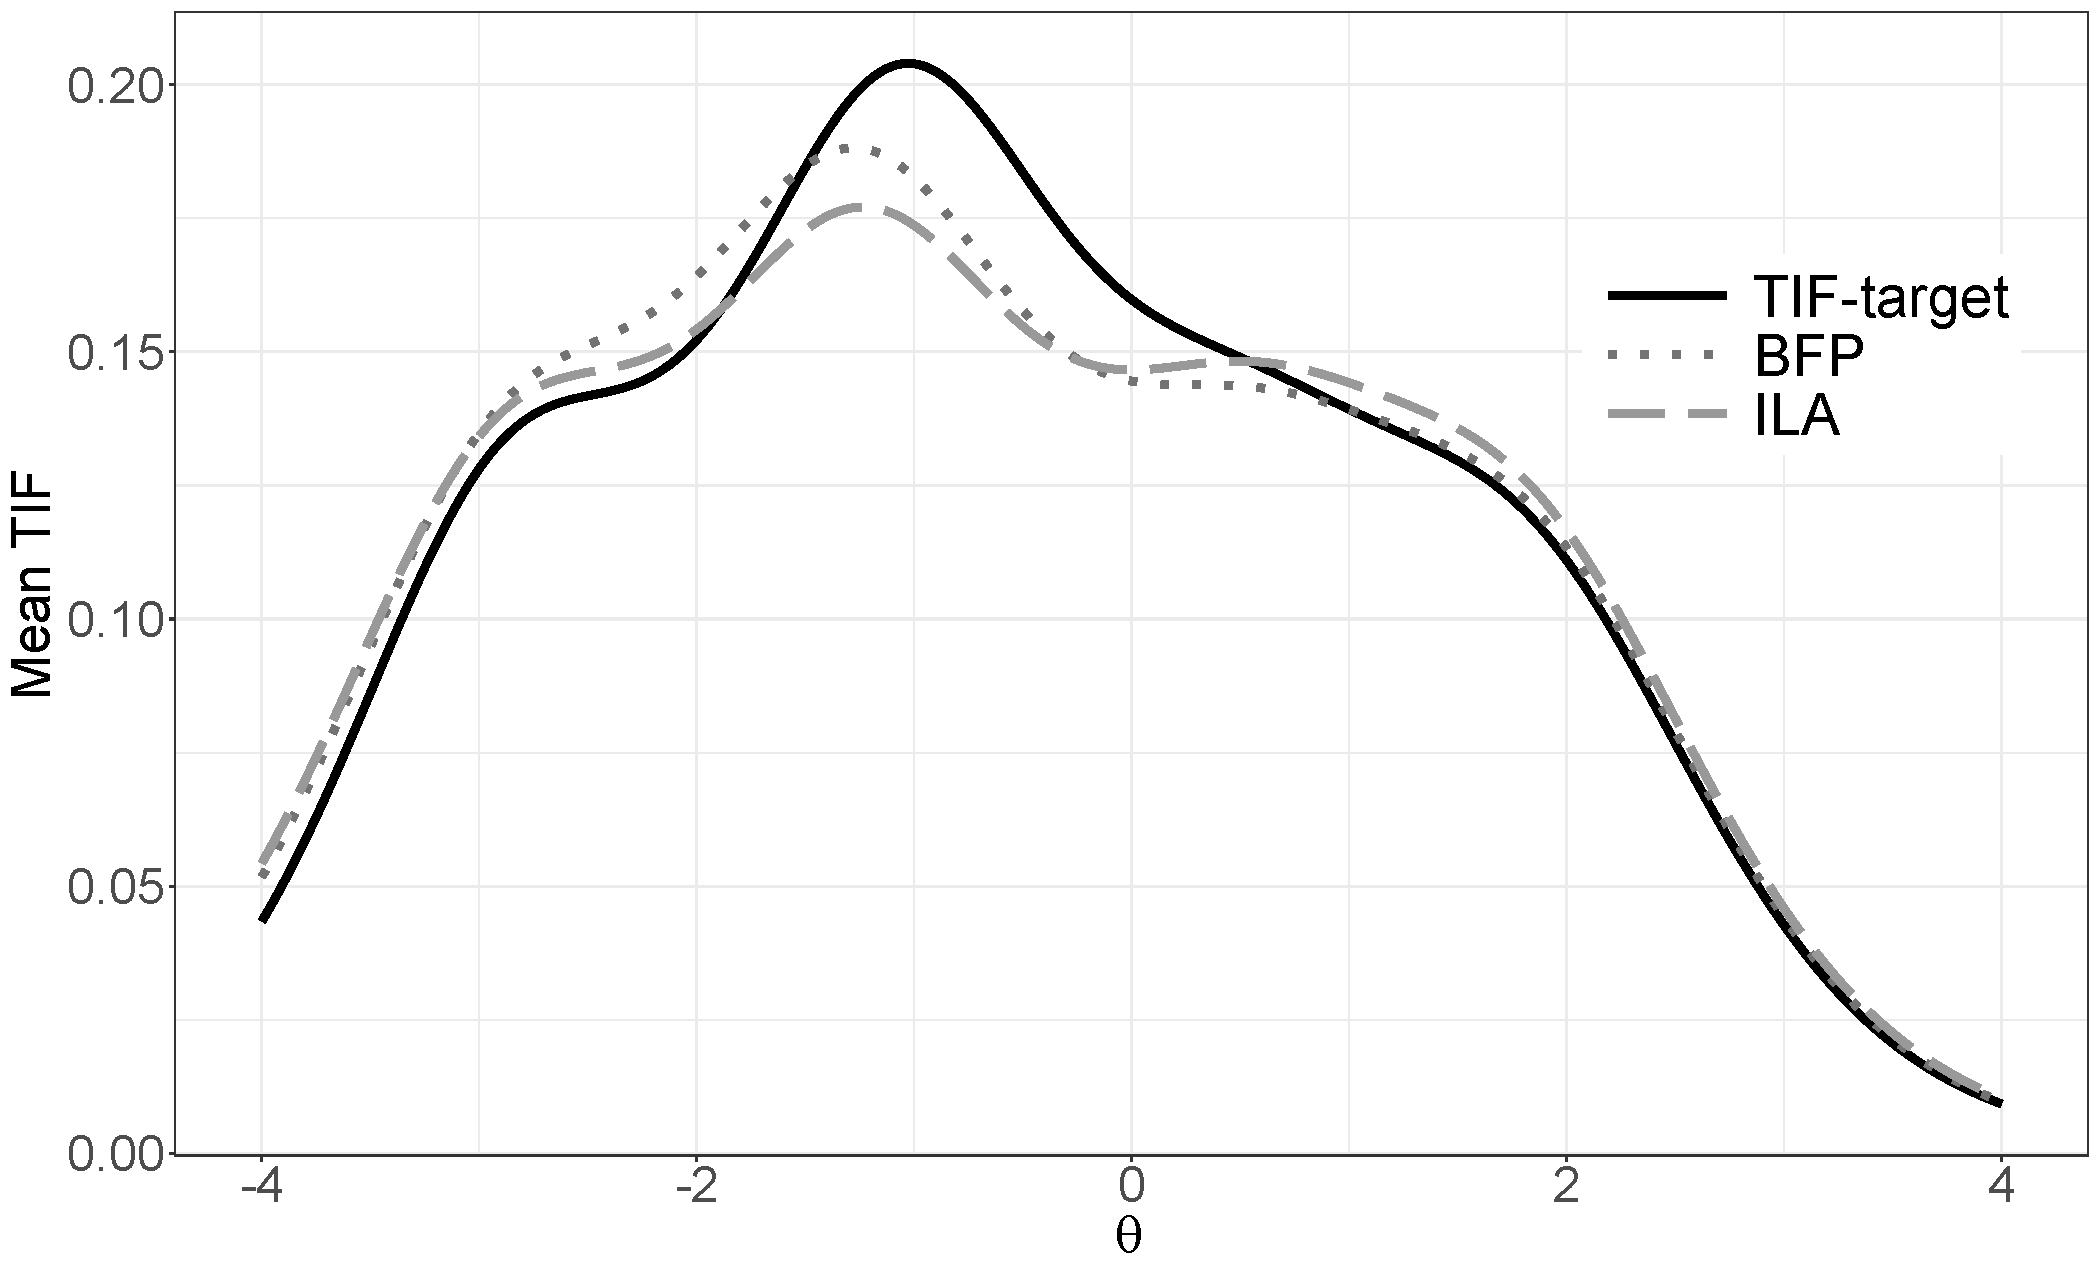
\includegraphics[width=.80\linewidth]{img/equalClose.pdf}	
			
			
			\centering
			\footnotesize{$||Q_{\text{BFP}}|| < ||Q_{\text{ILA}}||$, $RP = 3.17$}
			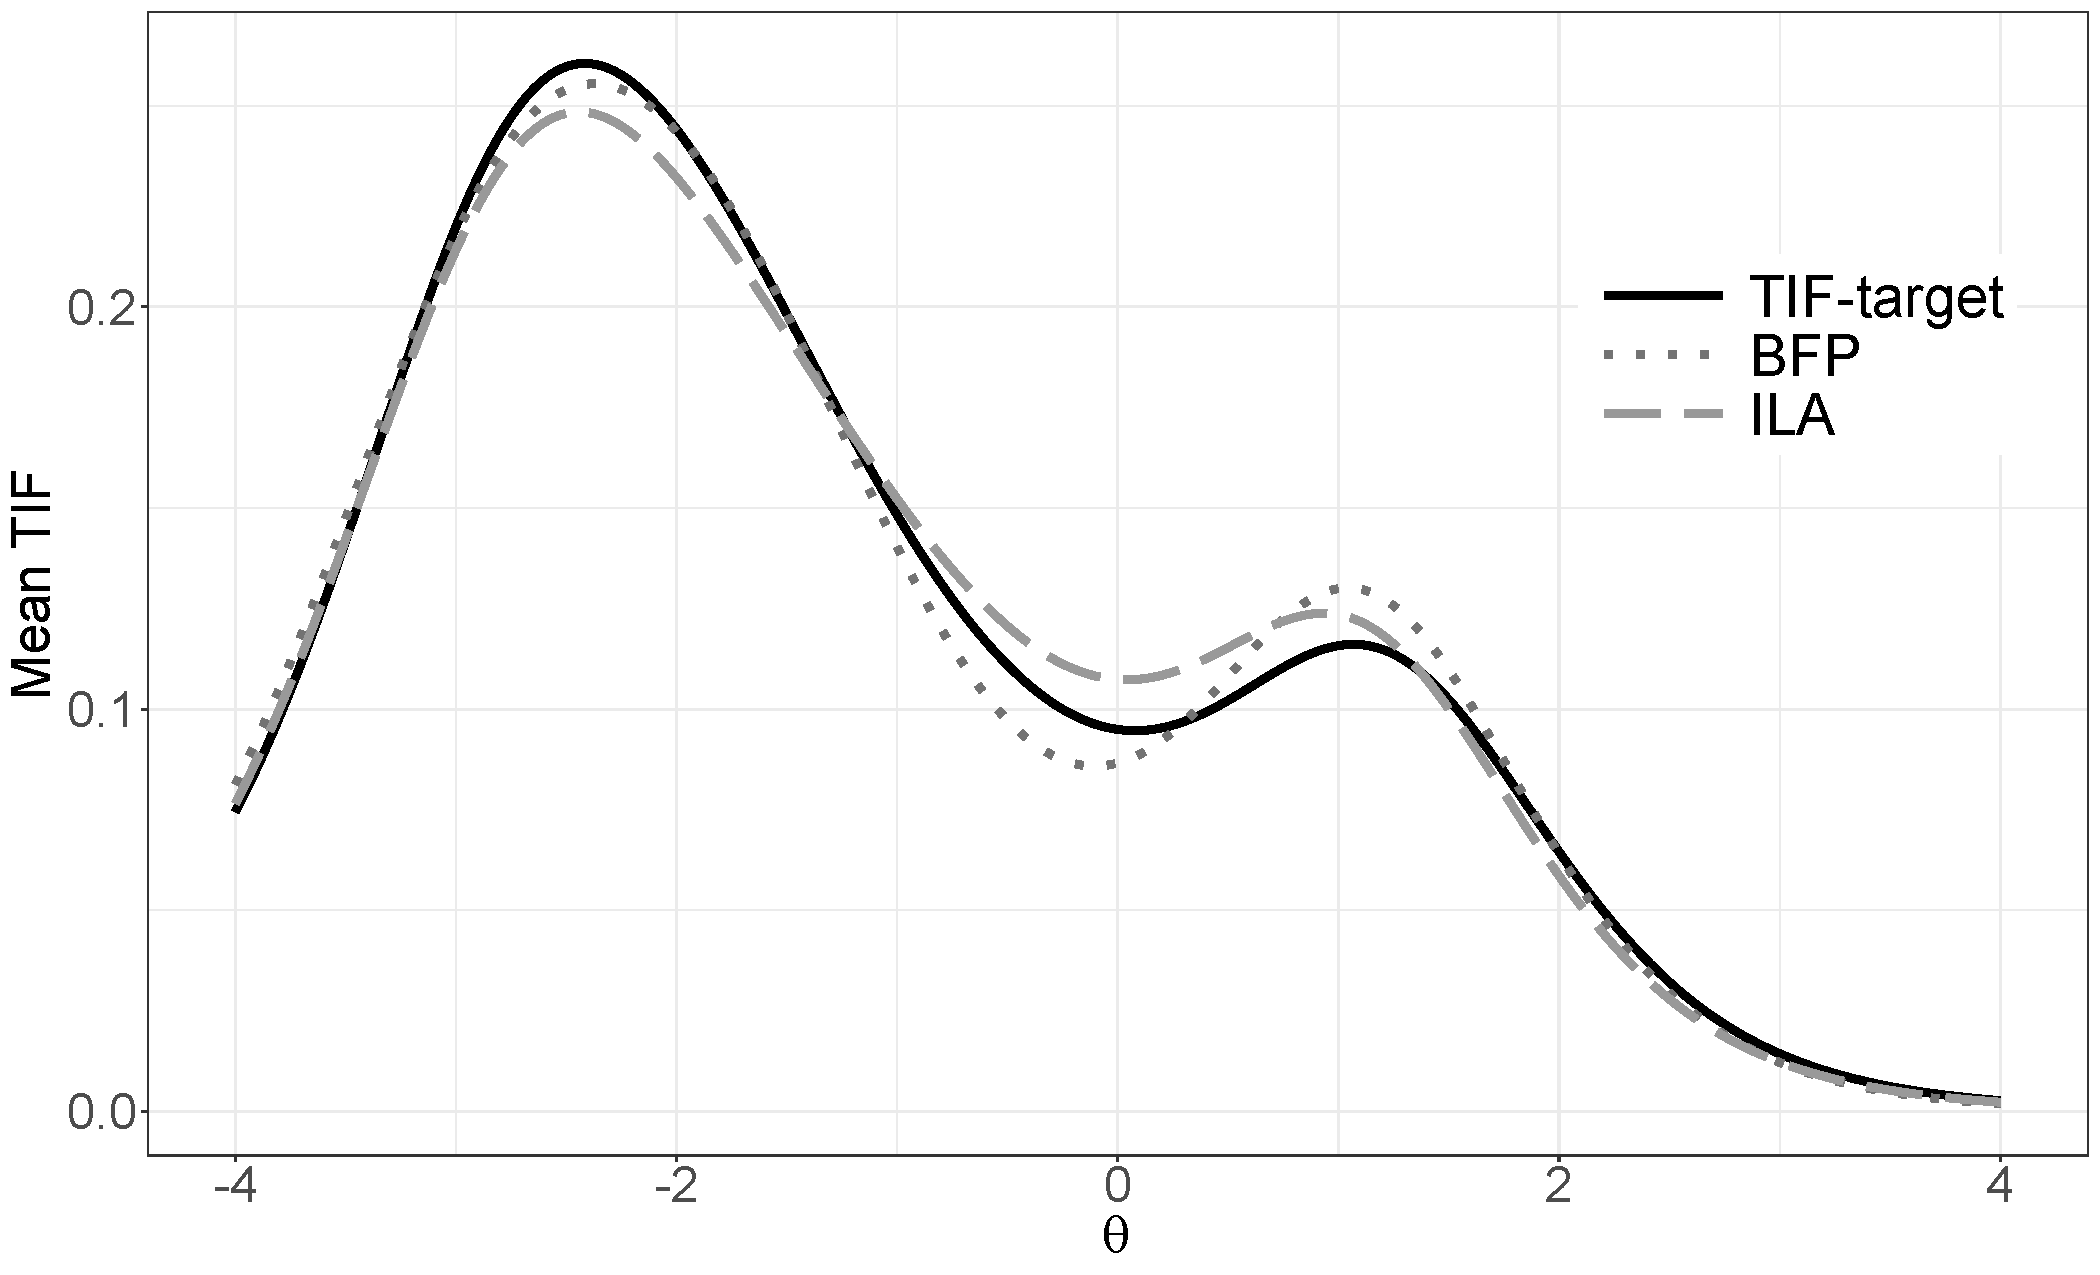
\includegraphics[width=.80\linewidth]{img/moreClose.pdf}	
			
			
			
		\end{column}
		
		\begin{column}{.50\linewidth}
			
			\centering
			\footnotesize{$||Q_{\text{BFP}}|| > ||Q_{\text{ILA}}||$, $RP = 4.76$}
			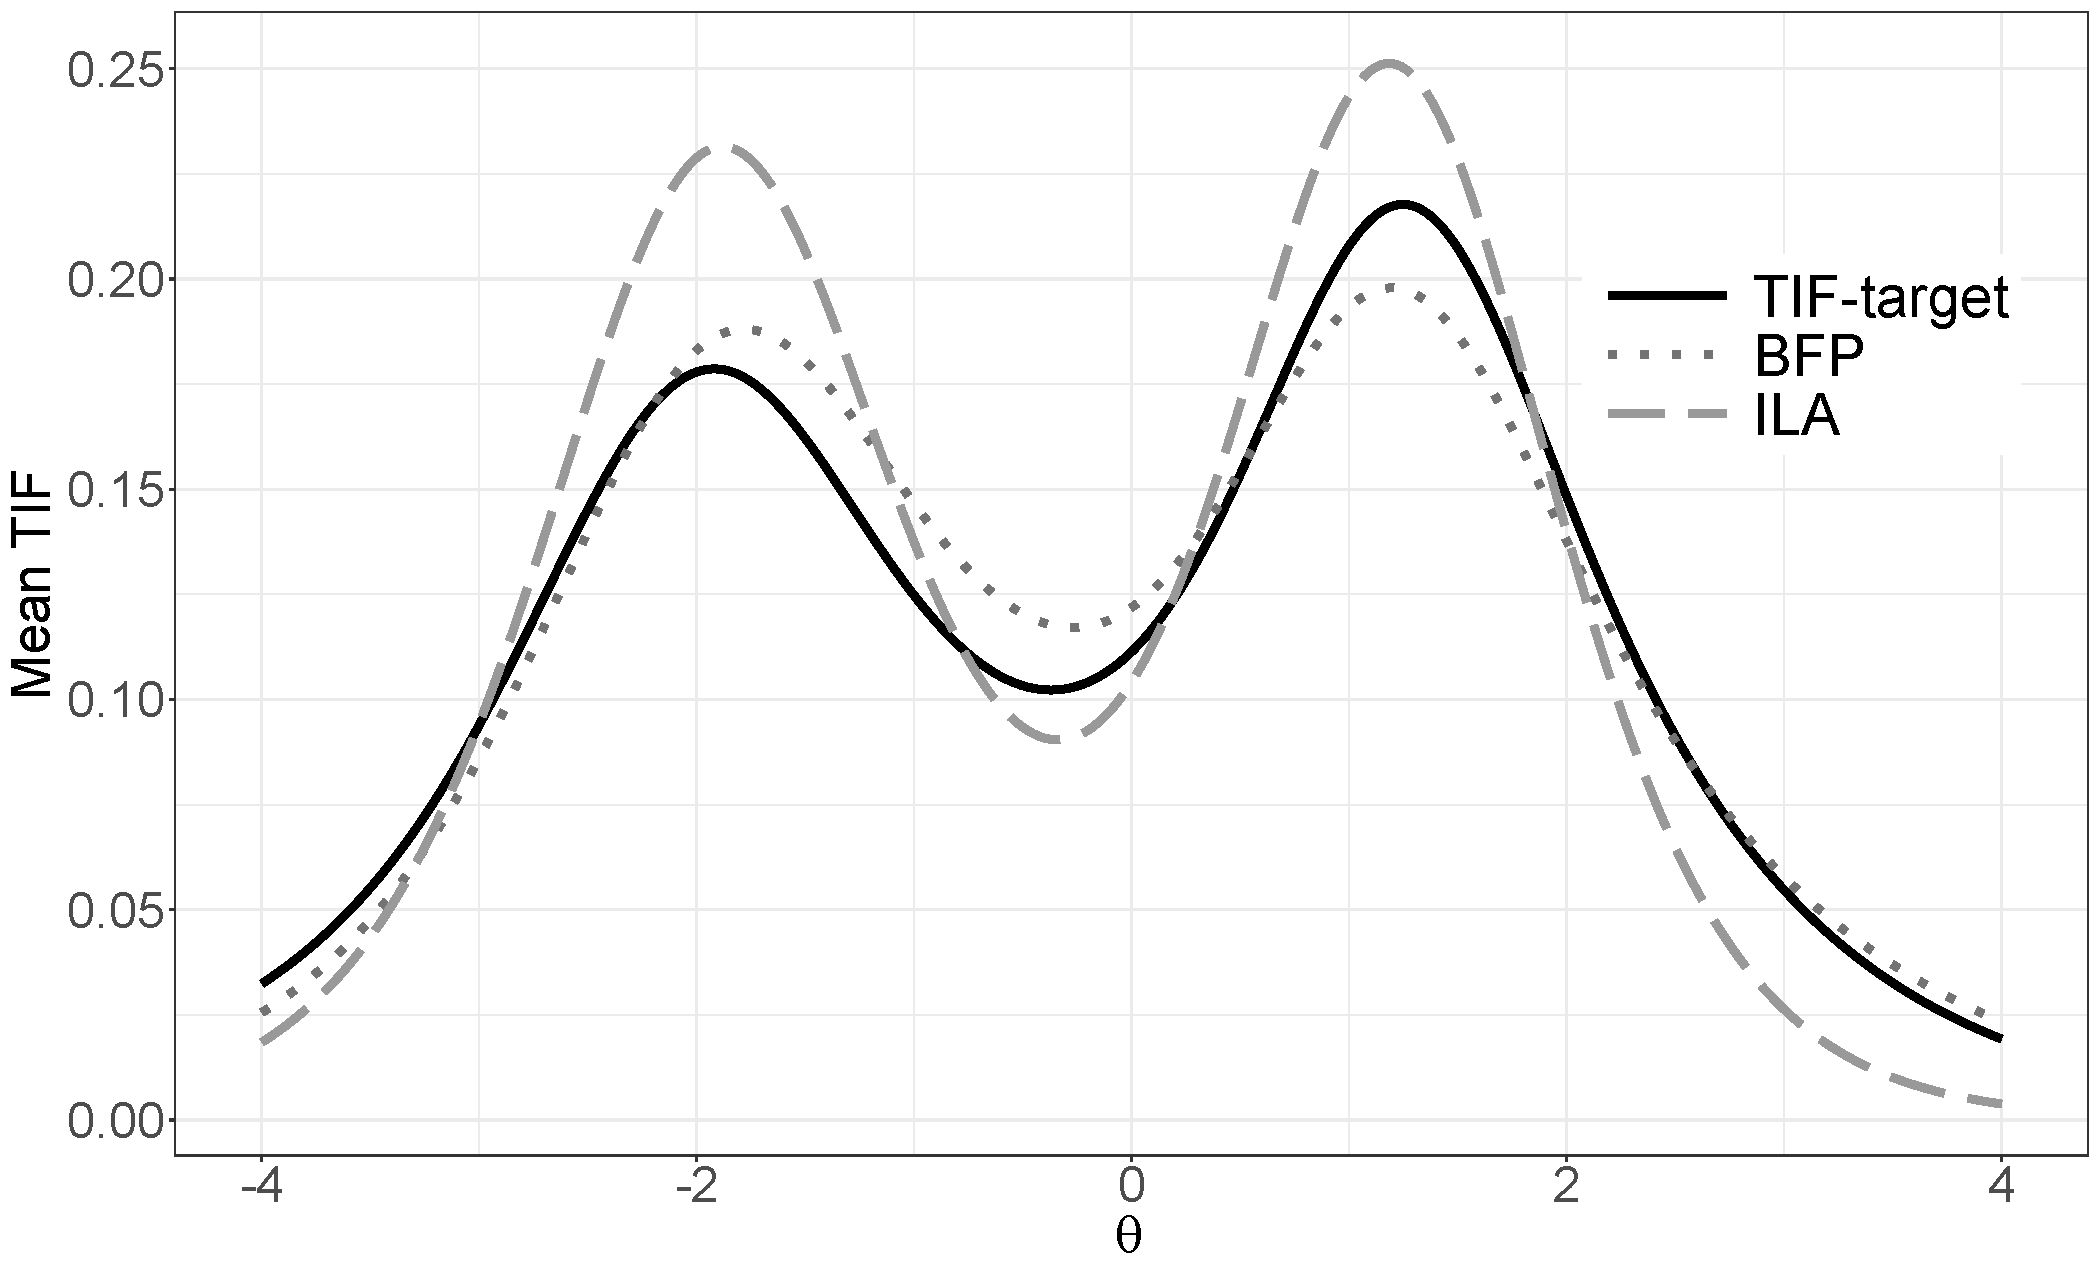
\includegraphics[width=.80\linewidth]{img/lessClose.pdf}	
			
			
			\centering
			\footnotesize{$||Q_{\text{BFP}}|| > ||Q_{\text{ILA}}||$, $RP=12.70$}
			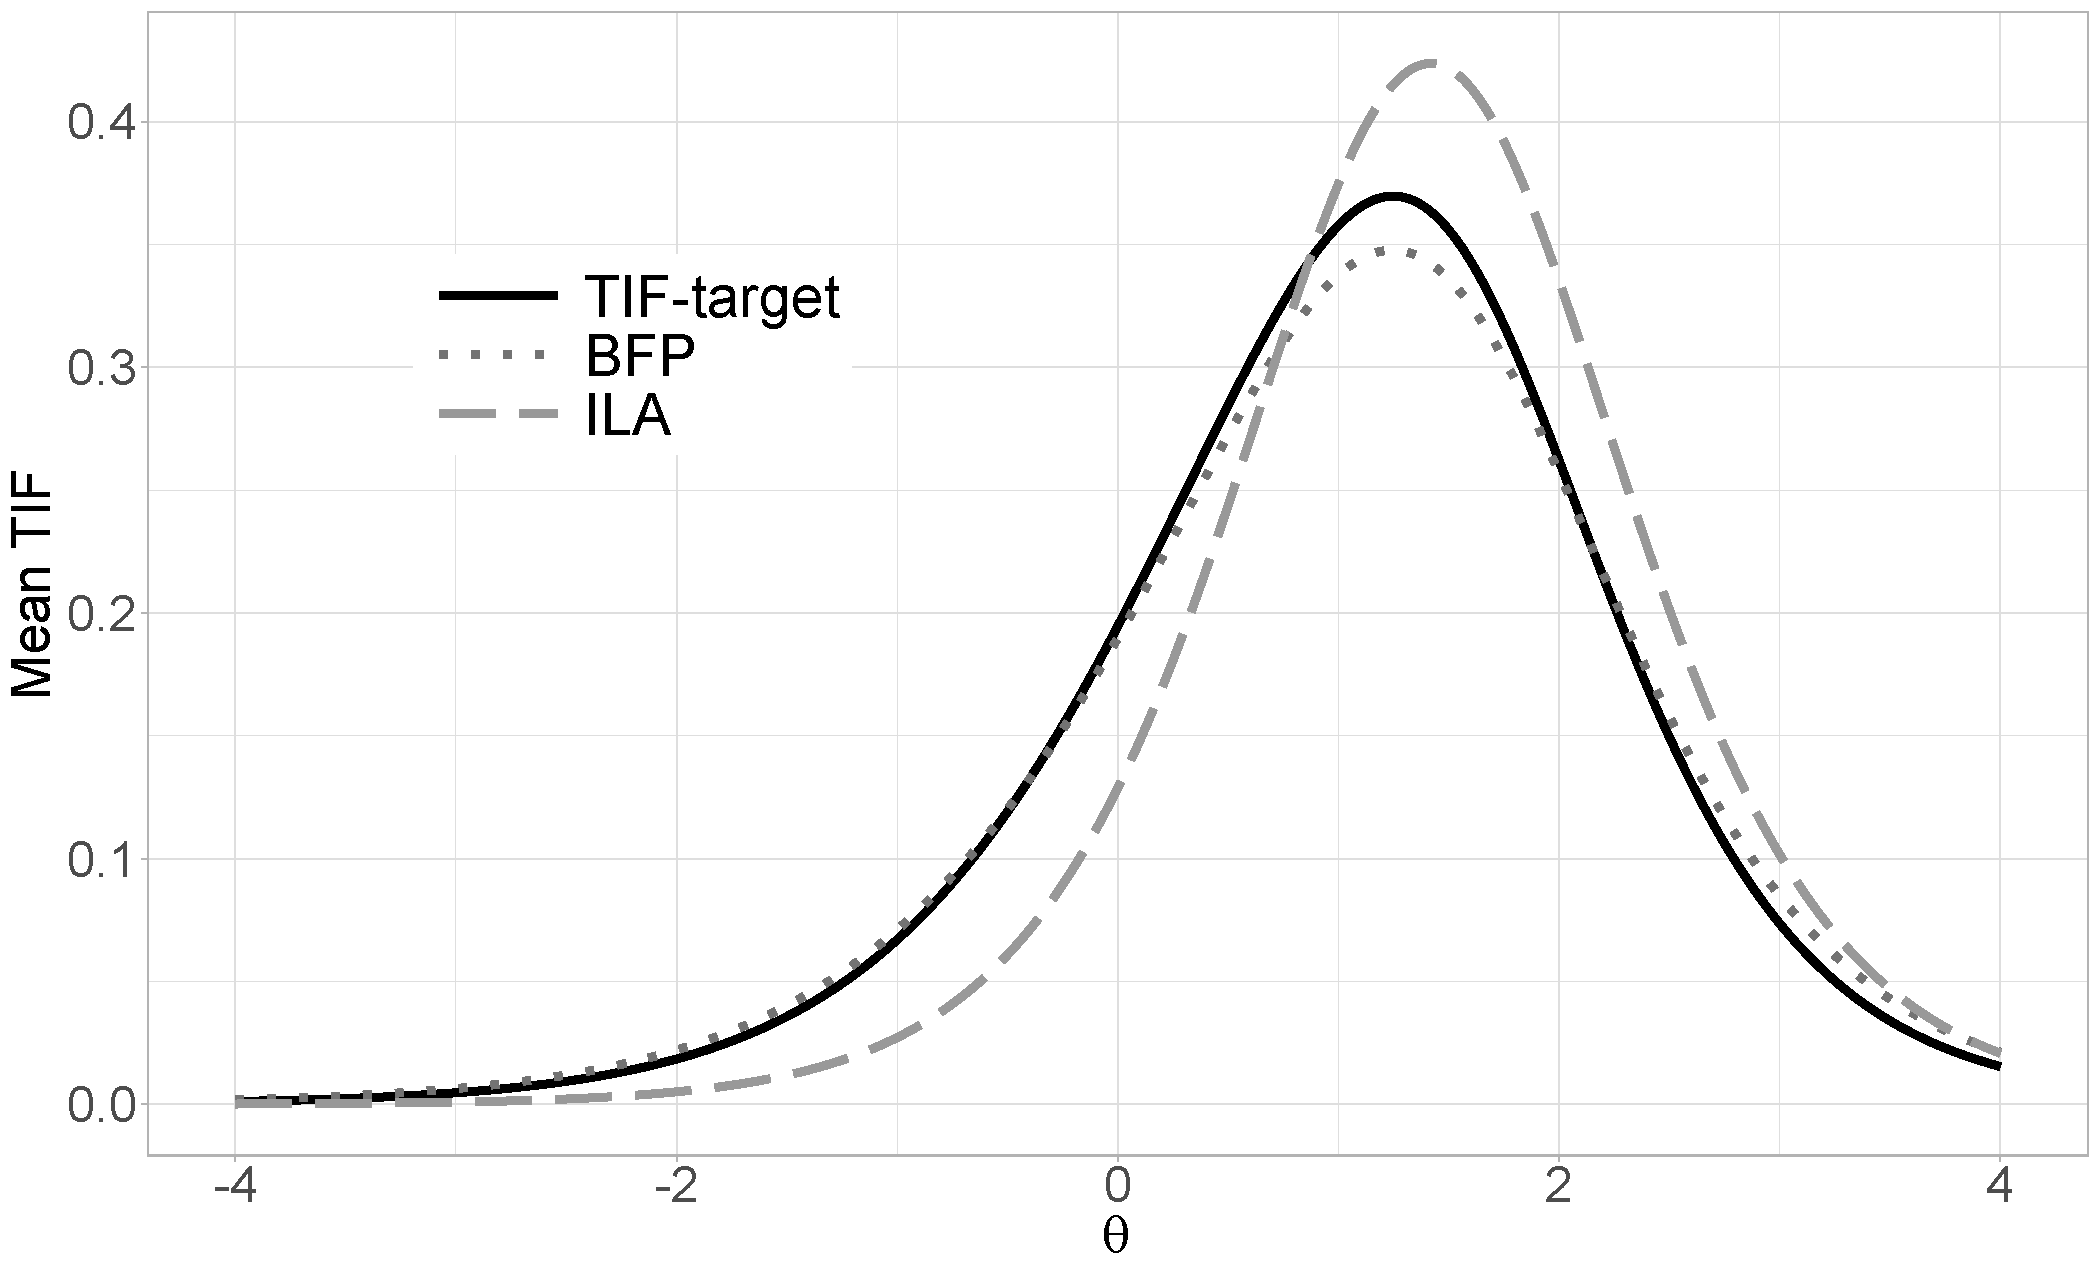
\includegraphics[width=.80\linewidth]{img/lessFar.pdf}	
			
			
		\end{column}
	\end{columns}
	
	
\end{frame}

\section{Wrapping up}


\begin{frame}
	\begin{itemize}
		\item IRT models and the information they provide are indeed useful for developing STFs
		\item There's not a one-fits-all solution, and all depends on: 
		\begin{itemize}
			\item The distribution of the latent trait (e.g., normal vs. skewed) 
			\item The aim of the assessment
			\item External constraints
		\end{itemize}
	\end{itemize}
	
	\textbf{Open questions}: 
	\begin{itemize}
		\item Is it convenient? 
		\item Where should we stop?
		\item Does it work on real data....?
	\end{itemize}
\end{frame}
\end{document}
